\documentclass[12pt]{amsart}
\usepackage[T1]{fontenc}
\usepackage[utf8]{inputenc}

\usepackage[top=1.95cm, bottom=1.95cm, left=2.35cm, right=2.35cm]{geometry}


\usepackage{wrapfig}

\usepackage{hyperref}
\usepackage{enumitem}
\usepackage{tcolorbox}
\usepackage{float}
\usepackage{cleveref}
\usepackage{multicol}
\usepackage{fancyvrb}
\usepackage{enumitem}
\usepackage{amsmath}
\usepackage{textcomp}
\usepackage[french]{babel}
\frenchsetup{StandardItemLabels=true}
\usepackage[
    type={CC},
    modifier={by-nc-sa},
	version={4.0},
]{doclicense}

\usepackage{tnsmath}

\DeclareMathOperator{\taille}{\tau}

\newtheorem{defi}{Définition}
\newtheorem{fact}{Fait}
\newtheorem*{proof*}{Preuve}

\newtheorem{remark}{Remarque}[section]

\NewDocumentCommand{\perim}{m}{\mathrm{Perim}(#1)}
\NewDocumentCommand{\area}{m}{\mathrm{Aire}(#1)}
\NewDocumentCommand{\garea}{m}{\mathrm{AireGe}(#1)}


\newcommand{\nline}{$n$-ligne}
\newcommand{\nlines}{$n$-lignes}

\newcommand{\kline}{$k$-ligne}
\newcommand{\klines}{$k$-lignes}


\newcommand{\ngone}{$n$-gone}
\newcommand{\ngones}{$n$-gones}

\newcommand{\kgone}{$k$-gone}
\newcommand{\kgones}{$k$-gones}

\newcommand{\niso}{$n$-isogone}
\newcommand{\nisos}{$n$-isogones}


\newcommand{\geogebra}{{\normalfont\texttt{GeoGebra}}}


\setlength\parindent{0pt}


\begin{document}

\title{BROUILLON - Inégalités isopérimétriques restreintes aux polygones}
\author{Christophe BAL}
\date{18 Jan. 2025 -- 3 Fev. 2025}
\maketitle


\begin{center}
	\hrule\vspace{.3em}
	{
		\fontsize{1.35em}{1em}\selectfont
		\textbf{Mentions \og légales \fg}
	}
			
	\vspace{0.45em}
	\doclicenseThis
	\hrule
\end{center}



\setcounter{tocdepth}{2}
\tableofcontents


% ------------- %


\newpage

%Ce document, qui se veut de niveau élémentaire,%
%\footnote{
%	Ceci nous amènera à admettre certains théorèmes faussement simples.
%}
%s'intéresse au classique problème de l'isopérimétrie plane, c'est-à-dire la recherche d'une surface plane maximisant son aire pour un périmètre fixé.
%Nous allons juste considérer le cas des polygones, tout en nous limitant à des preuves les plus géométriques possible.
%
%
%\begin{tcolorbox}
%	\itshape\small
%	Pour ne pas alourdir le texte, on raisonnera parfois modulo des isométries: on pourra parler \og \emph{du carré de côté $c$} \fg\kern-2pt, \og \emph{du triangle équilatéral de côté $c$} \fg\kern-2pt...
%\end{tcolorbox}
%
%
%% ------------- %
%
%
%\section{Triangles}
%
%\subsection{Avec un côté fixé}
%\begin{fact} \label{tri-one-side-fixed}
	Considérons tous les triangles de périmètre fixé, et ayant tous un côté en commun.
	Parmi tous ces triangles, il en existe un seul d'aire maximale, c'est le triangle isocèle ayant pour base le côté commun.
\end{fact}


\begin{proof}
	Soit $ABC$ un triangle de périmètre $p$, et fixons le côté $[AB]$. 
	Pour tout point $M$ sur la parallèle à $(AB)$ passant par $C$, nous savons que $\area{ABM} = \area{ABC}$. Notons alors $O$ le point sur cette parallèle tel que $ABO$ soit isocèle en $O$.

	\begin{center}
		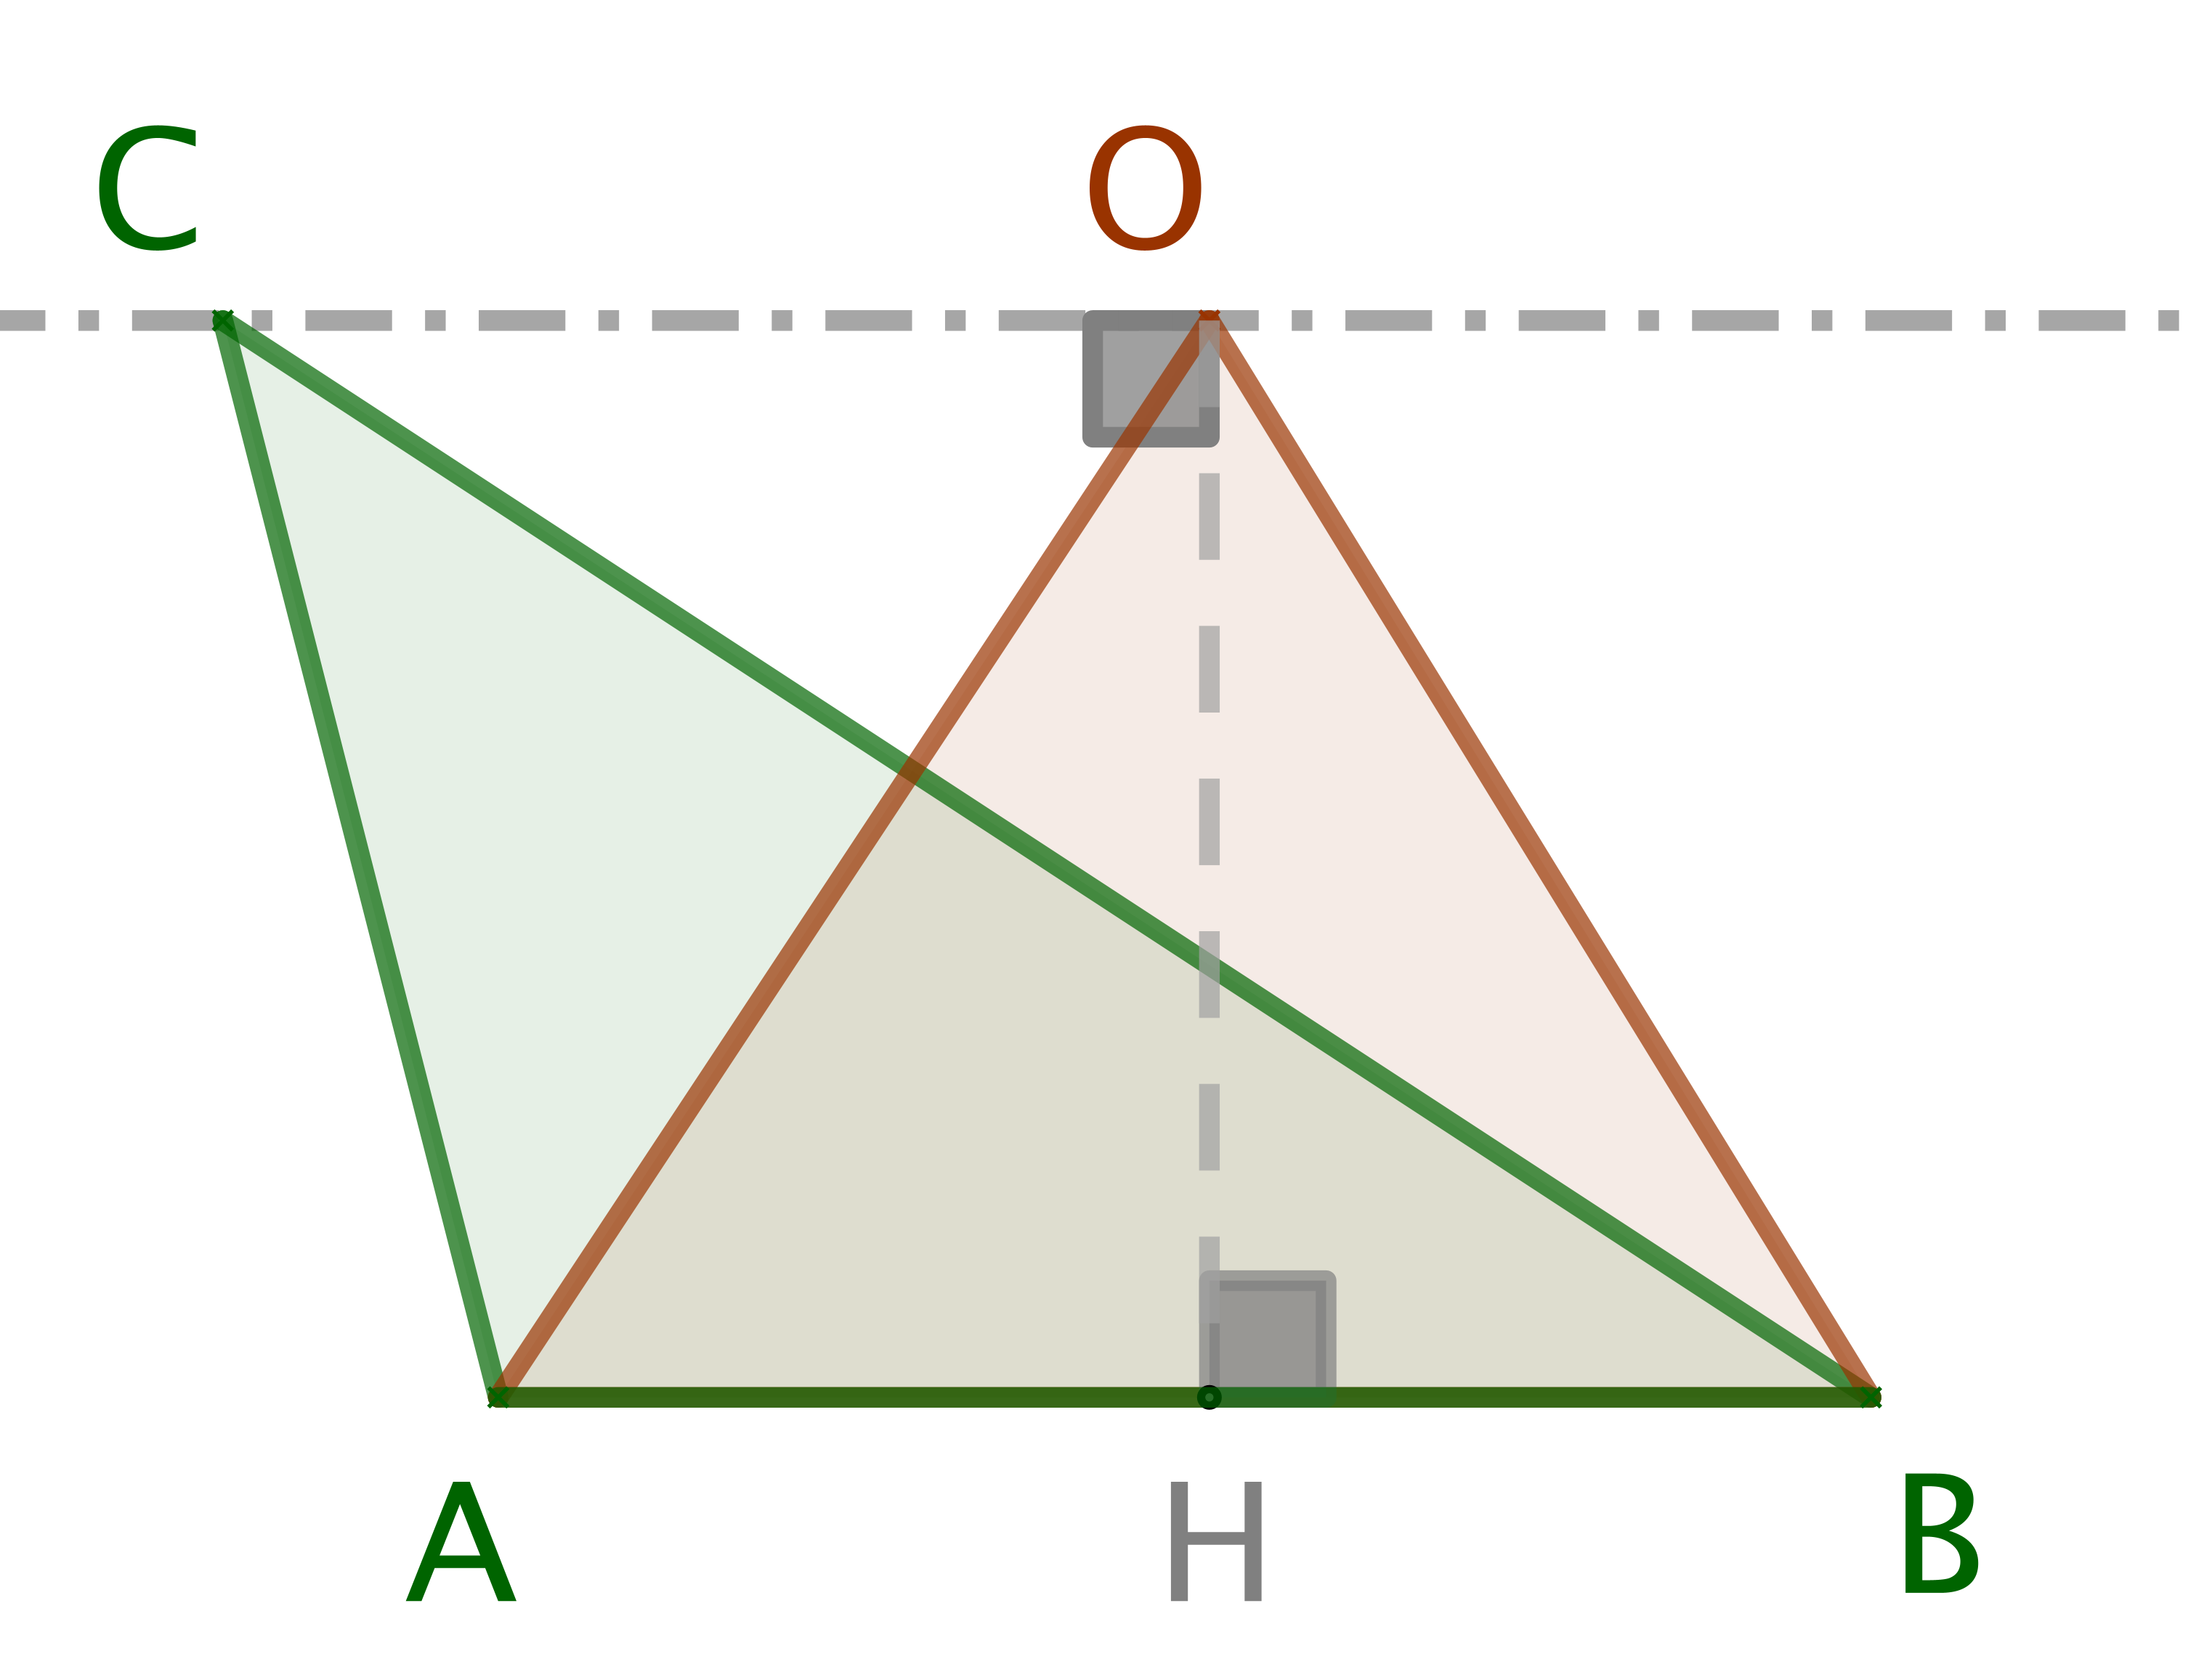
\includegraphics[scale=.4]{content/triangle-one-side-fixed/triangle.png}
	\end{center}

	
	Via une symétrie axiale, voir ci-dessous, il est aisé de noter que $\perim{ABC} \geq \perim{ABO}$, avec égalité uniquement si $ABC$ est isocèle en $C$.
	Plus précisément, en passant de $C$ à $O$, le périmètre diminue.
	
	\begin{center}
		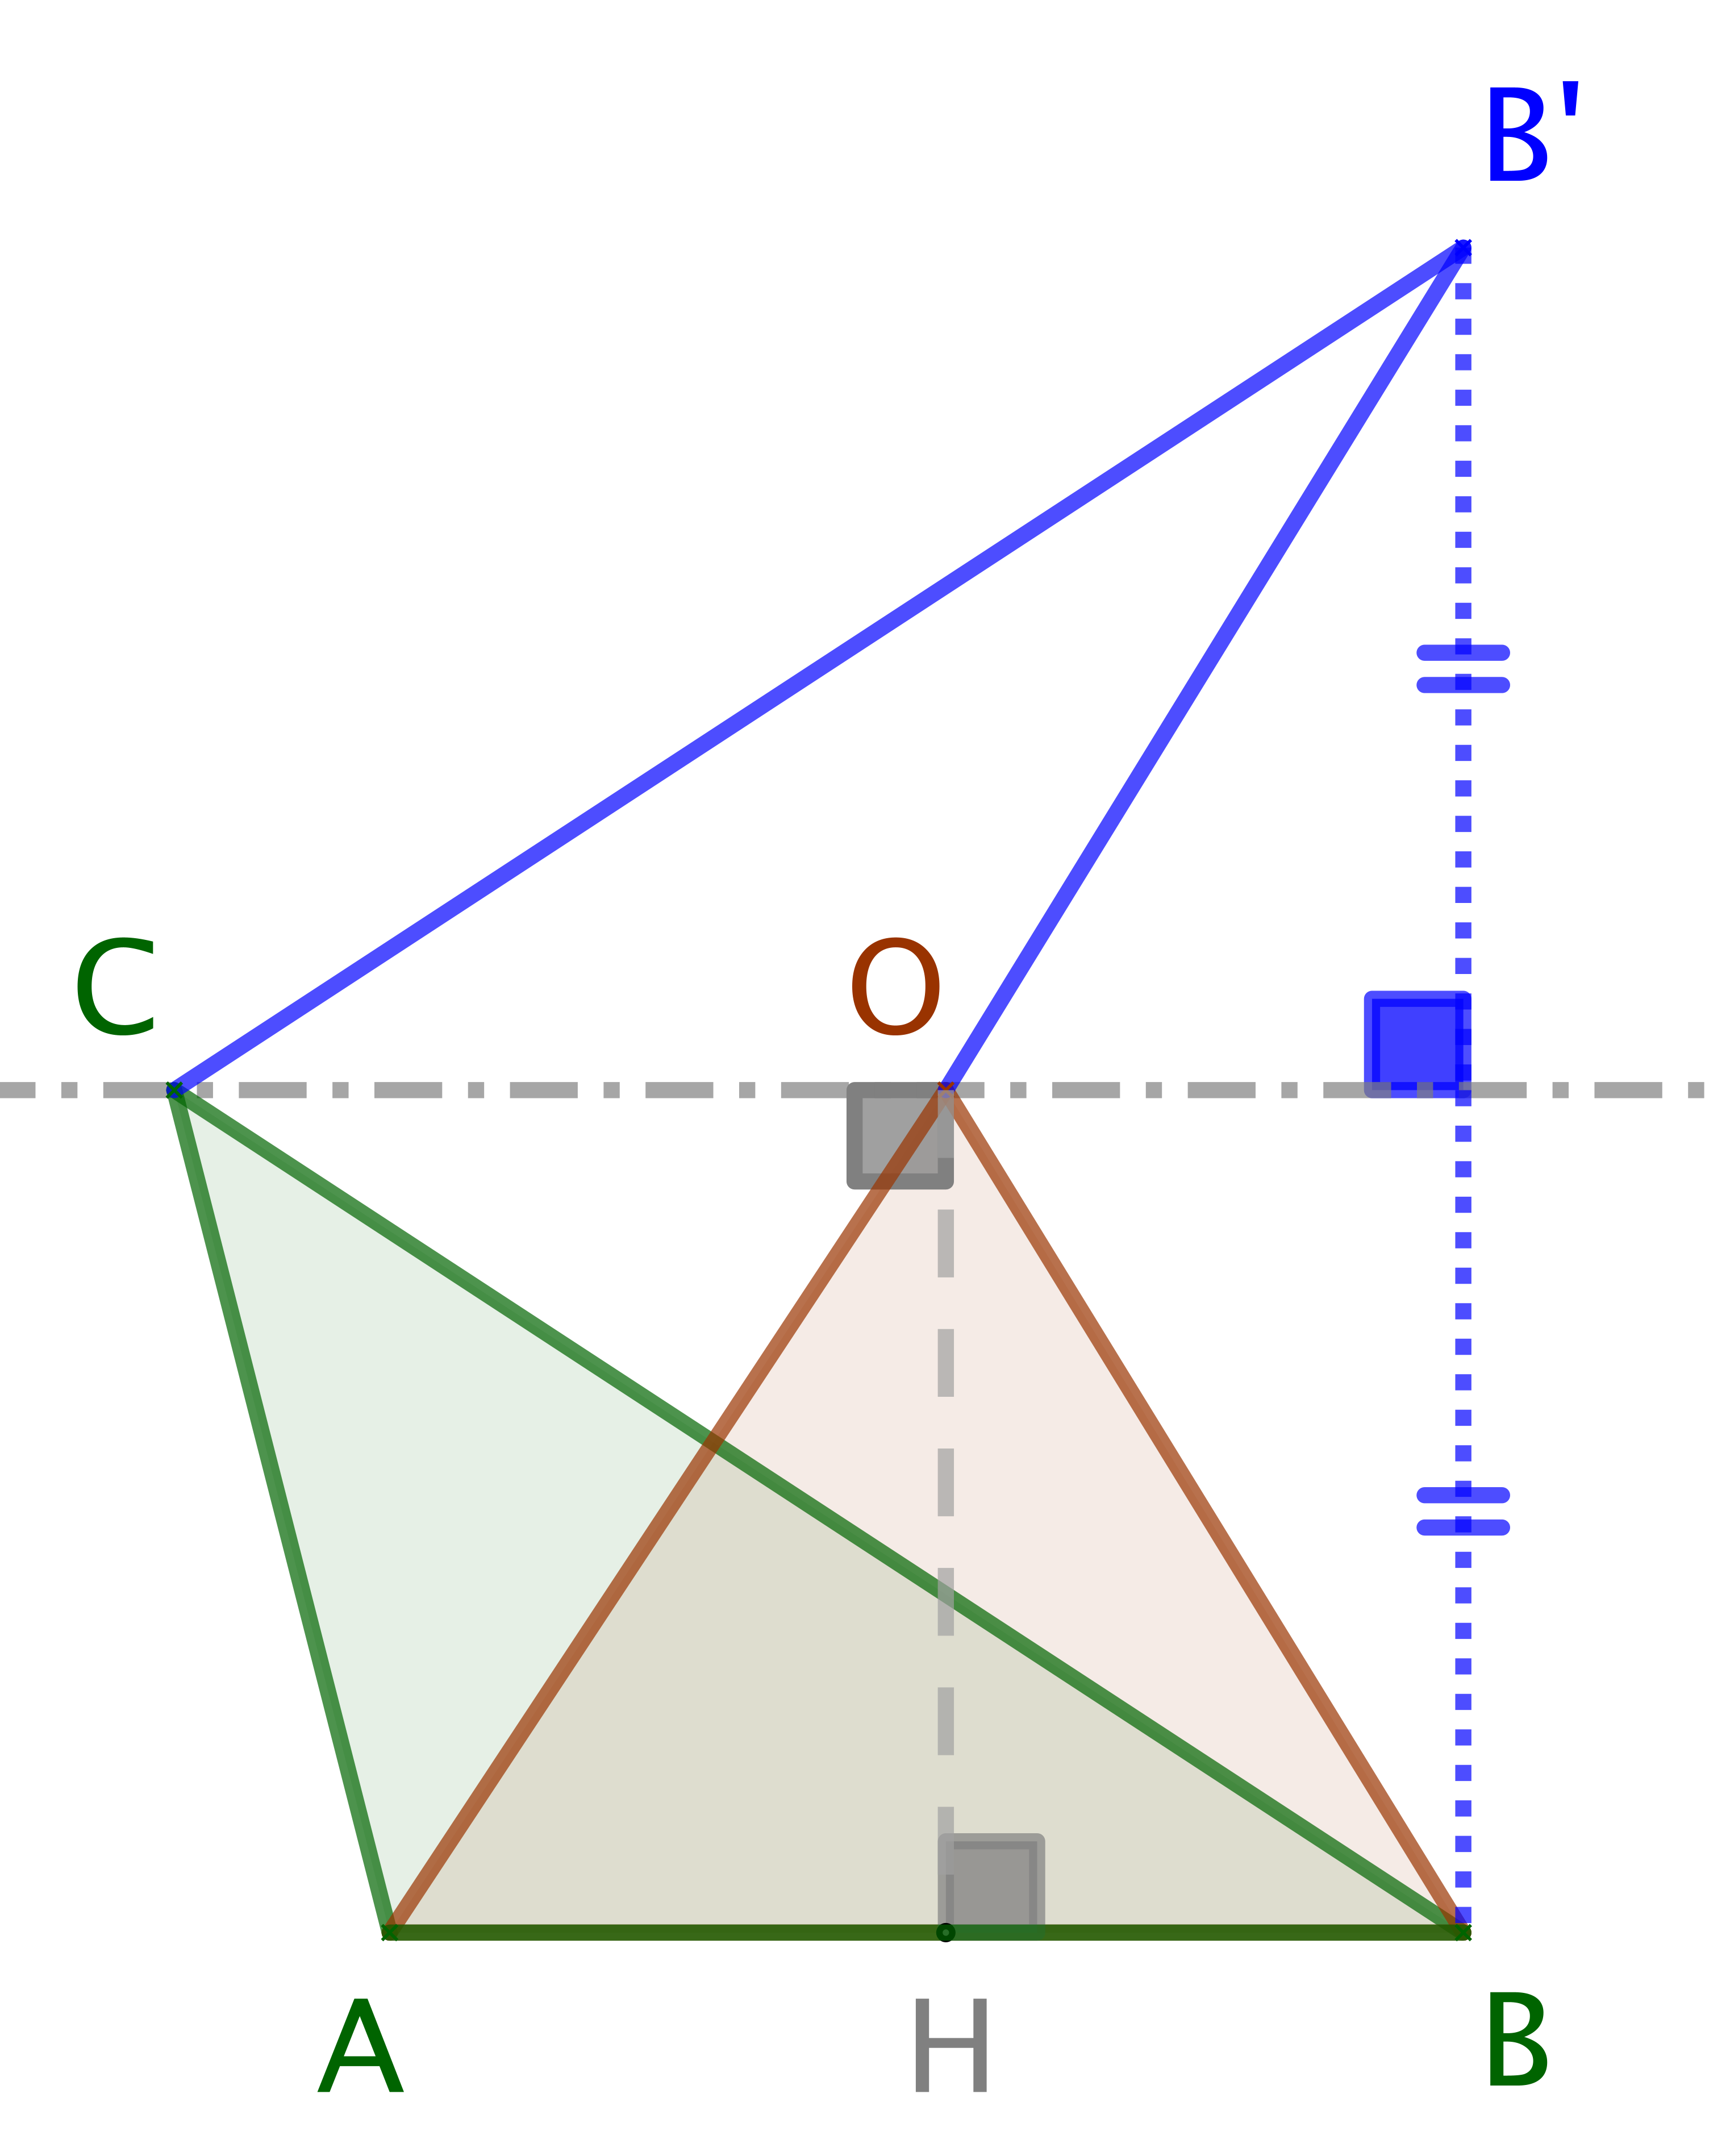
\includegraphics[scale=.4]{content/triangle-one-side-fixed/proof.png}
	\end{center}
	
	Une dilatation \focus{verticale} de rapport $r = \frac{\perim{ABC}}{\perim{ABO}} \geq 1$ donne un triangle isocèle $ABO^{\,\prime}$ tel que 
	$\perim{ABO^{\,\prime}} = p$
	et 
	$\area{ABO^{\,\prime}} \geq \area{ABC}$, avec égalité uniquement si $ABC$ est isocèle en $C$. 
	Contrat rempli!%
	\footnote{
		Dans la section \ref{constrained-extrema} est expliqué comment employer la méthode des extrema liés. 
		Les arguments fournis à cet endroit s'adaptent facilement au cas des triangles de base fixée.
	}
\end{proof}


% ----------------------- %


\begin{remark}
	La recherche parmi les triangles avec un côté fixé de celui ayant un périmètre minimal pour une aire fixée est le problème dual de l'isopérimétrie pour ces triangles.
\end{remark}

%
%
%\subsection{Le cas général}
%\begin{fact} \label{iso-tri}
	Considérons tous les triangles de périmètre fixé $p$. Parmi tous ces triangles, un seul est d'aire maximale, c'est le triangle équilatéral de côté $c = \dfrac13 p$.
\end{fact}


\begin{proof}	
	Nous allons donner une démonstration constructive via une application itérative du fait \ref{tri-one-side-fixed} qui va donner à la limite le triangle équilatéral d'aire maximale, et ceci avec une vitesse de convergence exponentielle.%
	\footnote{
		Ceci ne va nécessiter que l'emploi de propriétés simples de l'ensemble des réels.
	}
	Partons donc d'un triangle $ABC$ quelconque, mais de périmètre $p$, le fait \ref{tri-one-side-fixed} nous donne successivement les triangles $ACD$, $ADE$ et $AEF$ isocèles en $D$, $E$ et $F$ respectivement, ayant tous pour périmètre $p$, et ceci avec des aires de plus en plus grandes.  
	Le dessin suivant amène à conjecturer qu'en poursuivant le procédé pour avoir ensuite un triangle $AFG$ isocèle en $G$...\,, nous aboutirons \focus{à la limite} à un triangle équilatéral.

	\begin{center}
		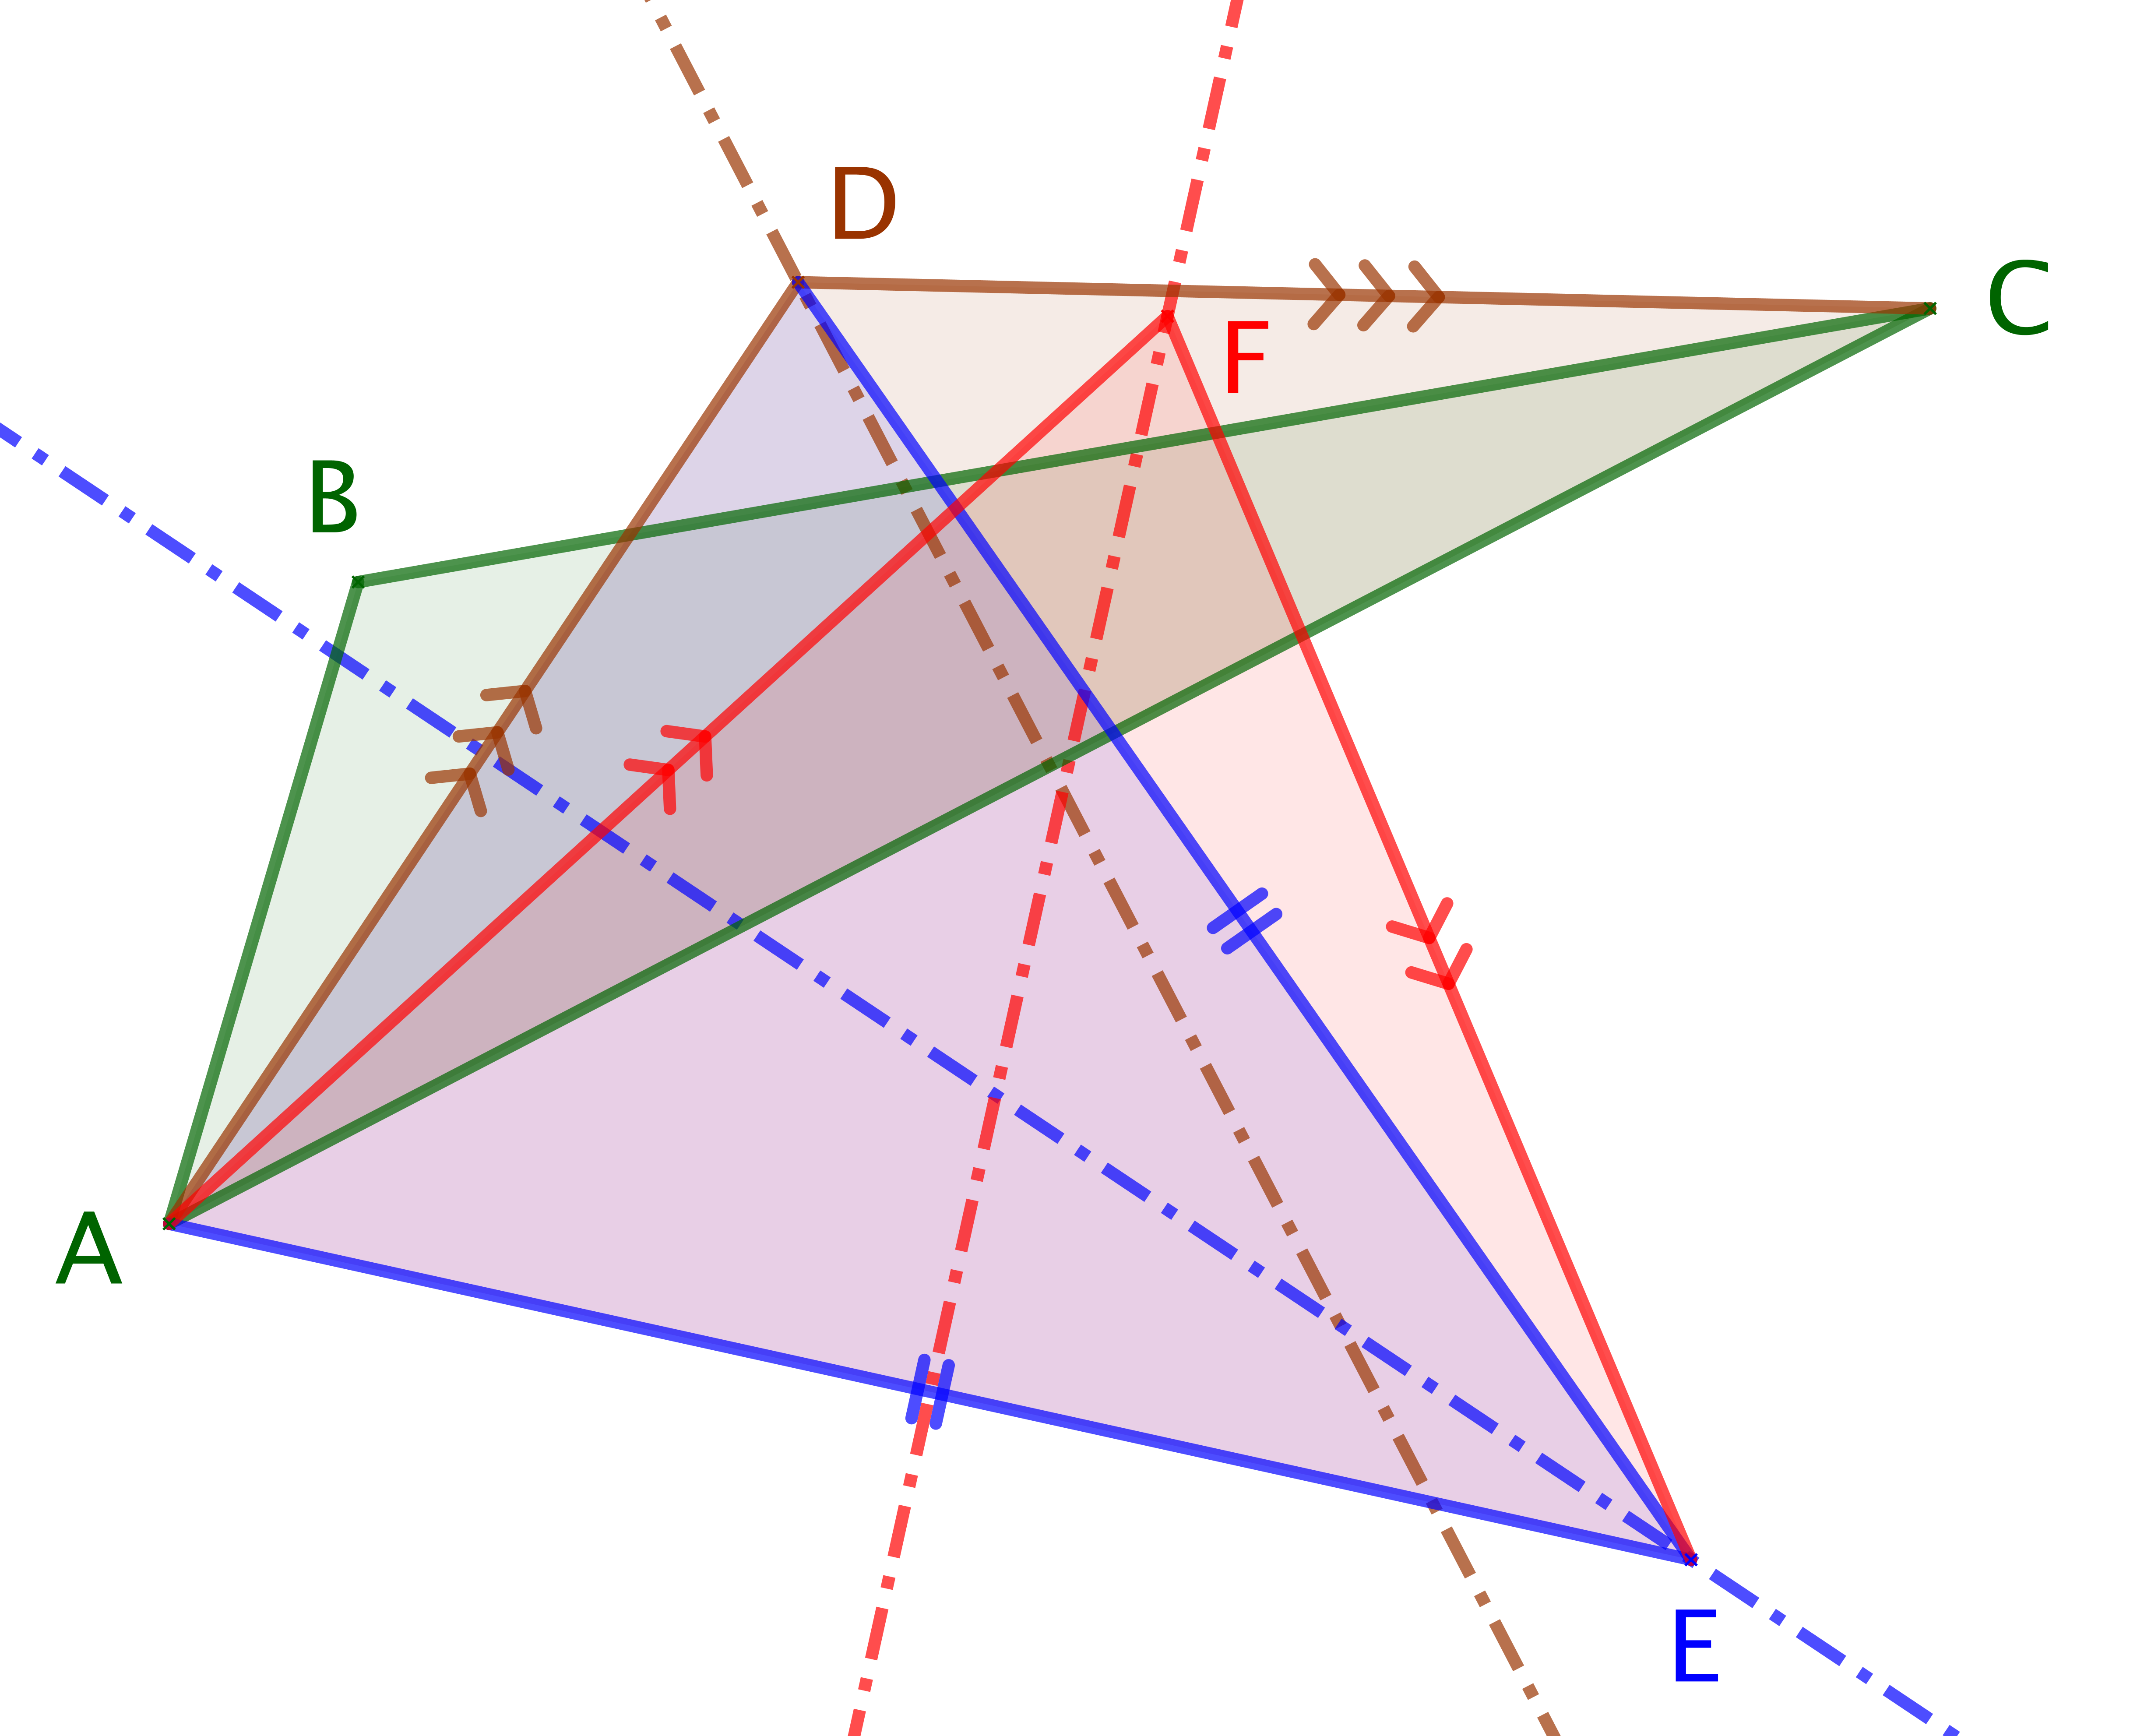
\includegraphics[scale=.4]{content/triangle-gene/proof.png}
	\end{center} 

	
	Le passage d'un triangle quelconque $ABC$ au triangle $ACD$ isocèle en $D$ nous amène à nous concentrer sur ce que donne notre procédé d'agrandissement d'aire à périmètre fixé pour des triangles isocèles. 
	Voici ce que nous pouvons affirmer en supposant $AC > AD$, comme dans notre exemple (nous allons voir que cette hypothèse est sans conséquence).
	%
	\begin{enumerate}
		\item Comme $AC + 2 AD = p$ et $AC > AD$, nous avons $AC > \frac13 p > AD$.
		À l'étape suivante, comme $AD + 2 AE = p$, nous obtenons $AD < \frac13 p < AE$.


		\item Pour $AEF$ isocèle en $F$, comme $AE + 2AF = p$, nous arrivons à  $AE > \frac13 p > AF$.
		
		
		\item \label{tri-equi-conv}
		Tentons de quantifier les écarts à la mesure pivot $p^{\,\prime} = \frac13 p$. 
		%
		\begin{itemize}
			\item Dans $ACD$, posant $AD = p^{\,\prime} - \epsilon_1$, nous avons $AC = p^{\,\prime} + 2 \epsilon_1$.

			\item Dans $ADE$, posant $AE = p^{\,\prime} + \epsilon_2$, nous avons $AD = p^{\,\prime} - 2 \epsilon_2$.

			\item Dans $AEF$, posant $AF = p^{\,\prime} - \epsilon_3$, nous avons $AE = p^{\,\prime} + 2 \epsilon_3$.

			\item Dans $AFG$, posant $AG = p^{\,\prime} + \epsilon_4$, nous avons $AF = p^{\,\prime} - 2 \epsilon_4$.

			\item Donc
			$\epsilon_2 = \frac12 \epsilon_1$,
			$\epsilon_3 = \frac12 \epsilon_2$
			et
			$\epsilon_4 = \frac12 \epsilon_3$.
		\end{itemize}
	\end{enumerate}


	\smallskip
	
	Voici les enseignements de ce qui précède en partant d'un triangle $ABC$ non équilatéral.
	%
	\begin{itemize}
		\item Si $AC = \frac13p$, dès la 1\iere\ itération, nous avons un triangle équilatéral d'aire plus grande.
		
		
		\item Si $AC \neq \frac13p$, notre procédé n'arrivera jamais en un nombre fini d'étapes à un triangle équilatéral.
		Dans ce cas, le point \ref{tri-equi-conv} ci-dessus nous donne une convergence exponentielle des longueurs des côtés vers $p^{\,\prime} = \frac13 p$, tout en ayant des aires des plus en plus grandes.
	\end{itemize}
	
	Dans tous les cas, l'aire d'un triangle non équilatéral de périmètre $p$ est strictement majorée par celle du triangle équilatéral de périmètre $p$. Et tout ceci a été obtenu via de la géométrie et de l'analyse élémentaires!
\end{proof}

%
%
%% ------------- %
%
%
%\section{Quadriltères}
%
%\subsection{Les rectangles}
%\begin{fact} \label{iso-rect}
	Considérons tous les rectangles de périmètre fixé $p$. Parmi tous ces rectangles, celui d'aire maximale est le carré de côté $c = \num{.25} p$.
\end{fact}


\begin{proof}
	Une preuve courante est d'exprimer l'aire du rectangle comme un polynôme du 2\ieme\ degré en $L$ par exemple.%
	\footnote{
		L'aire est donnée par $L \ell = L (\num{.5} p - L)$ qui est maximale en $L_M = \num{.25} p$ (moyenne des racines), d'où $\ell_M = \num{.25} p = L_M$.
	}
	On peut en fait faire plus simplement grâce au dessin suivant où les rectangles $1$, $2$ et $3$ sont isométriques au rectangle vert étudié de dimension $L \times \ell$.

	\begin{center}
		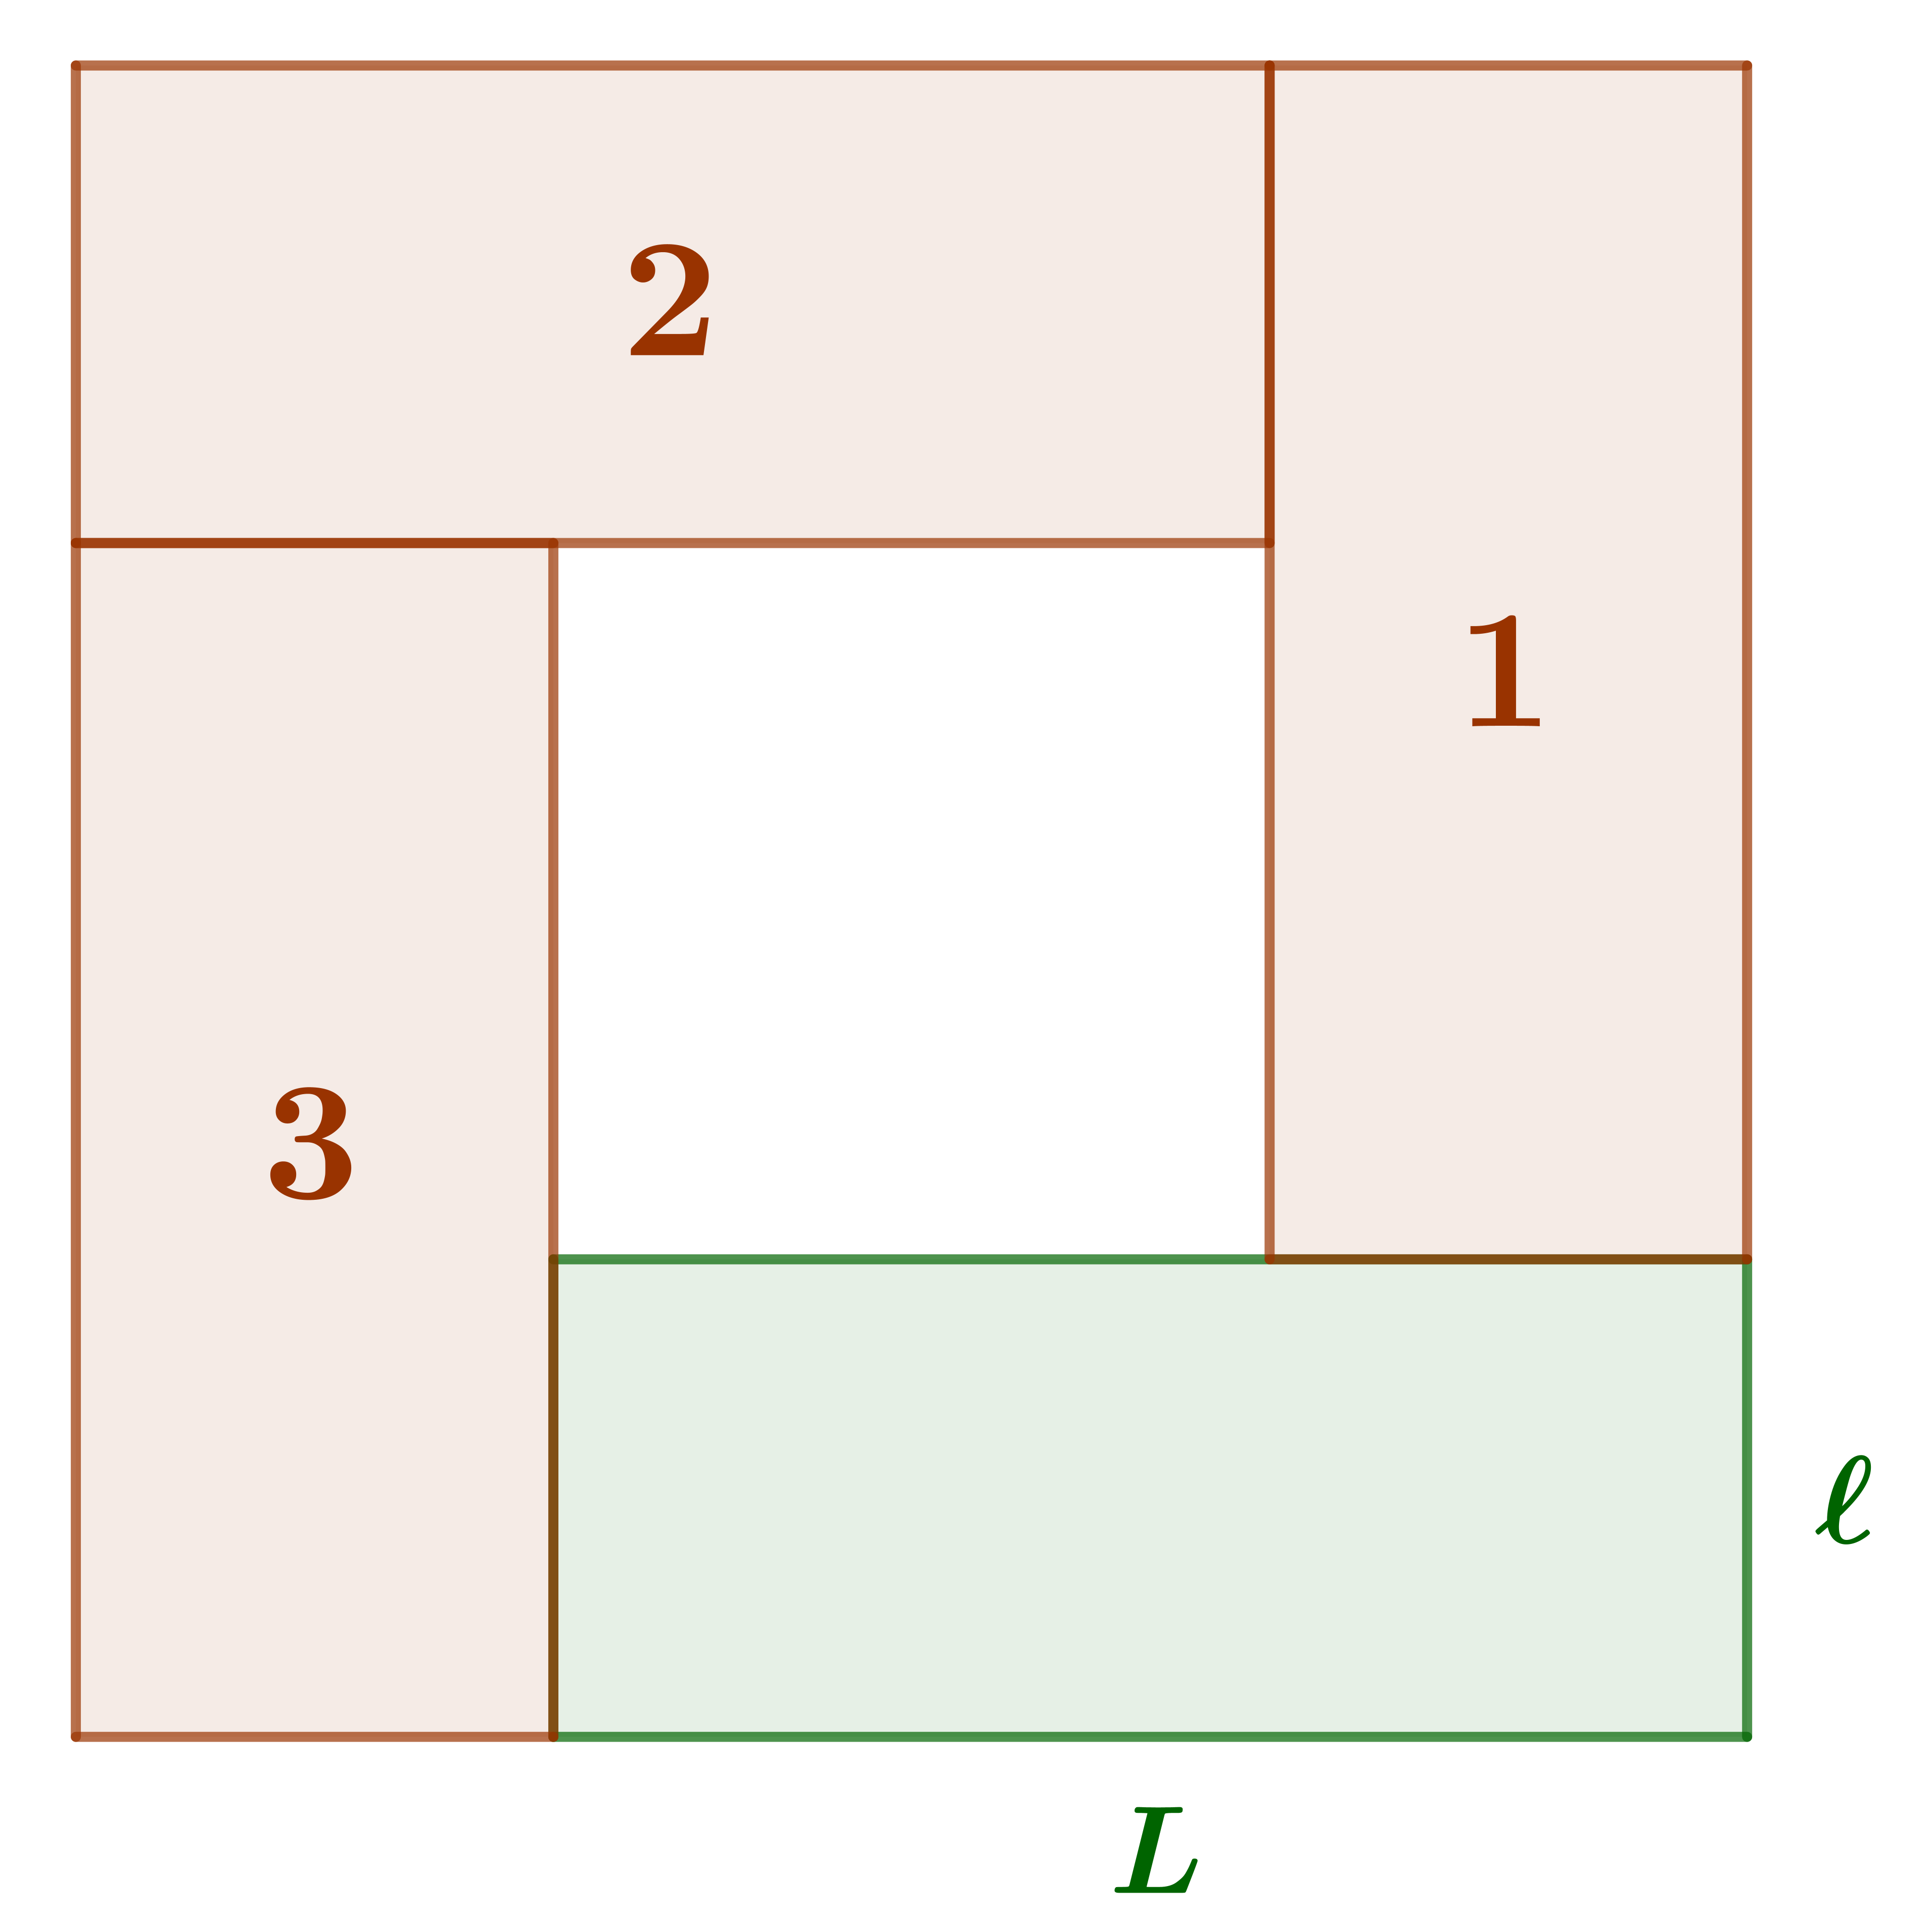
\includegraphics[scale=.4]{content/rectangle/rectangle.png}
	\end{center}
	
	Le raisonnement tient alors aux constations suivantes accessibles à un collégien.
	%
	\begin{enumerate}
		\item Le grand carré a une aire supérieure ou égale à $4 L \ell$.

		\item Le grand carré a un périmètre égal à $4 (L + \ell)$.

		\item Via une homothétie de rapport \num{.5}\,, nous obtenons un carré d'aire supérieure ou égale à $\num{.5}^2 \times 4 L \ell =  L \ell$, et de périmètre égal à $\num{.5} \times 4 (L + \ell) = 2 (L + \ell)$.
	\end{enumerate}
	
	Donc pour tout rectangle de périmètre $p = 2 (L + \ell)$ et d'aire $L \ell$, nous pouvons construire un carré de périmètre identique, mais avec une aire supérieure ou égale à  $L \ell$. Joli! Non?
\end{proof}


\begin{remark}
	Au passage, nous avons pour $(L ; \ell) \in \big( \RRsp \big)^2$, $4 L \ell \leq (L + \ell)^2$, c'est-à-dire $2 L \ell \leq L^2 + \ell^2$, d'où $\sqrt{L \ell} \leq \sqrt{\frac12 (L^2 + \ell^2)}$, soit la comparaison des moyennes géométriques et quadratiques d'ordre $2$.
\end{remark}

%
%
%\subsection{Les parallélogrammes}
%\begin{fact} \label{iso-para}
	Considérons tous les parallélogrammes de périmètre fixé $p$. Parmi tous ces parallélogrammes, un seul est d'aire maximale, c'est le carré de côté $c = \num{.25} p$.
\end{fact}


\begin{proof}
	Le calcul de l'aire d'un parallélogramme, voir le dessin ci-dessous, nous donne 
	$\area{ABCD} = \area{ABHH^{\,\prime}}$ et 
	$\perim{ABCD} \geq \perim{ABHH^{\,\prime}}$, 
	avec égalité uniquement si $ABCD$ est un rectangle. 
	
	\begin{center}
		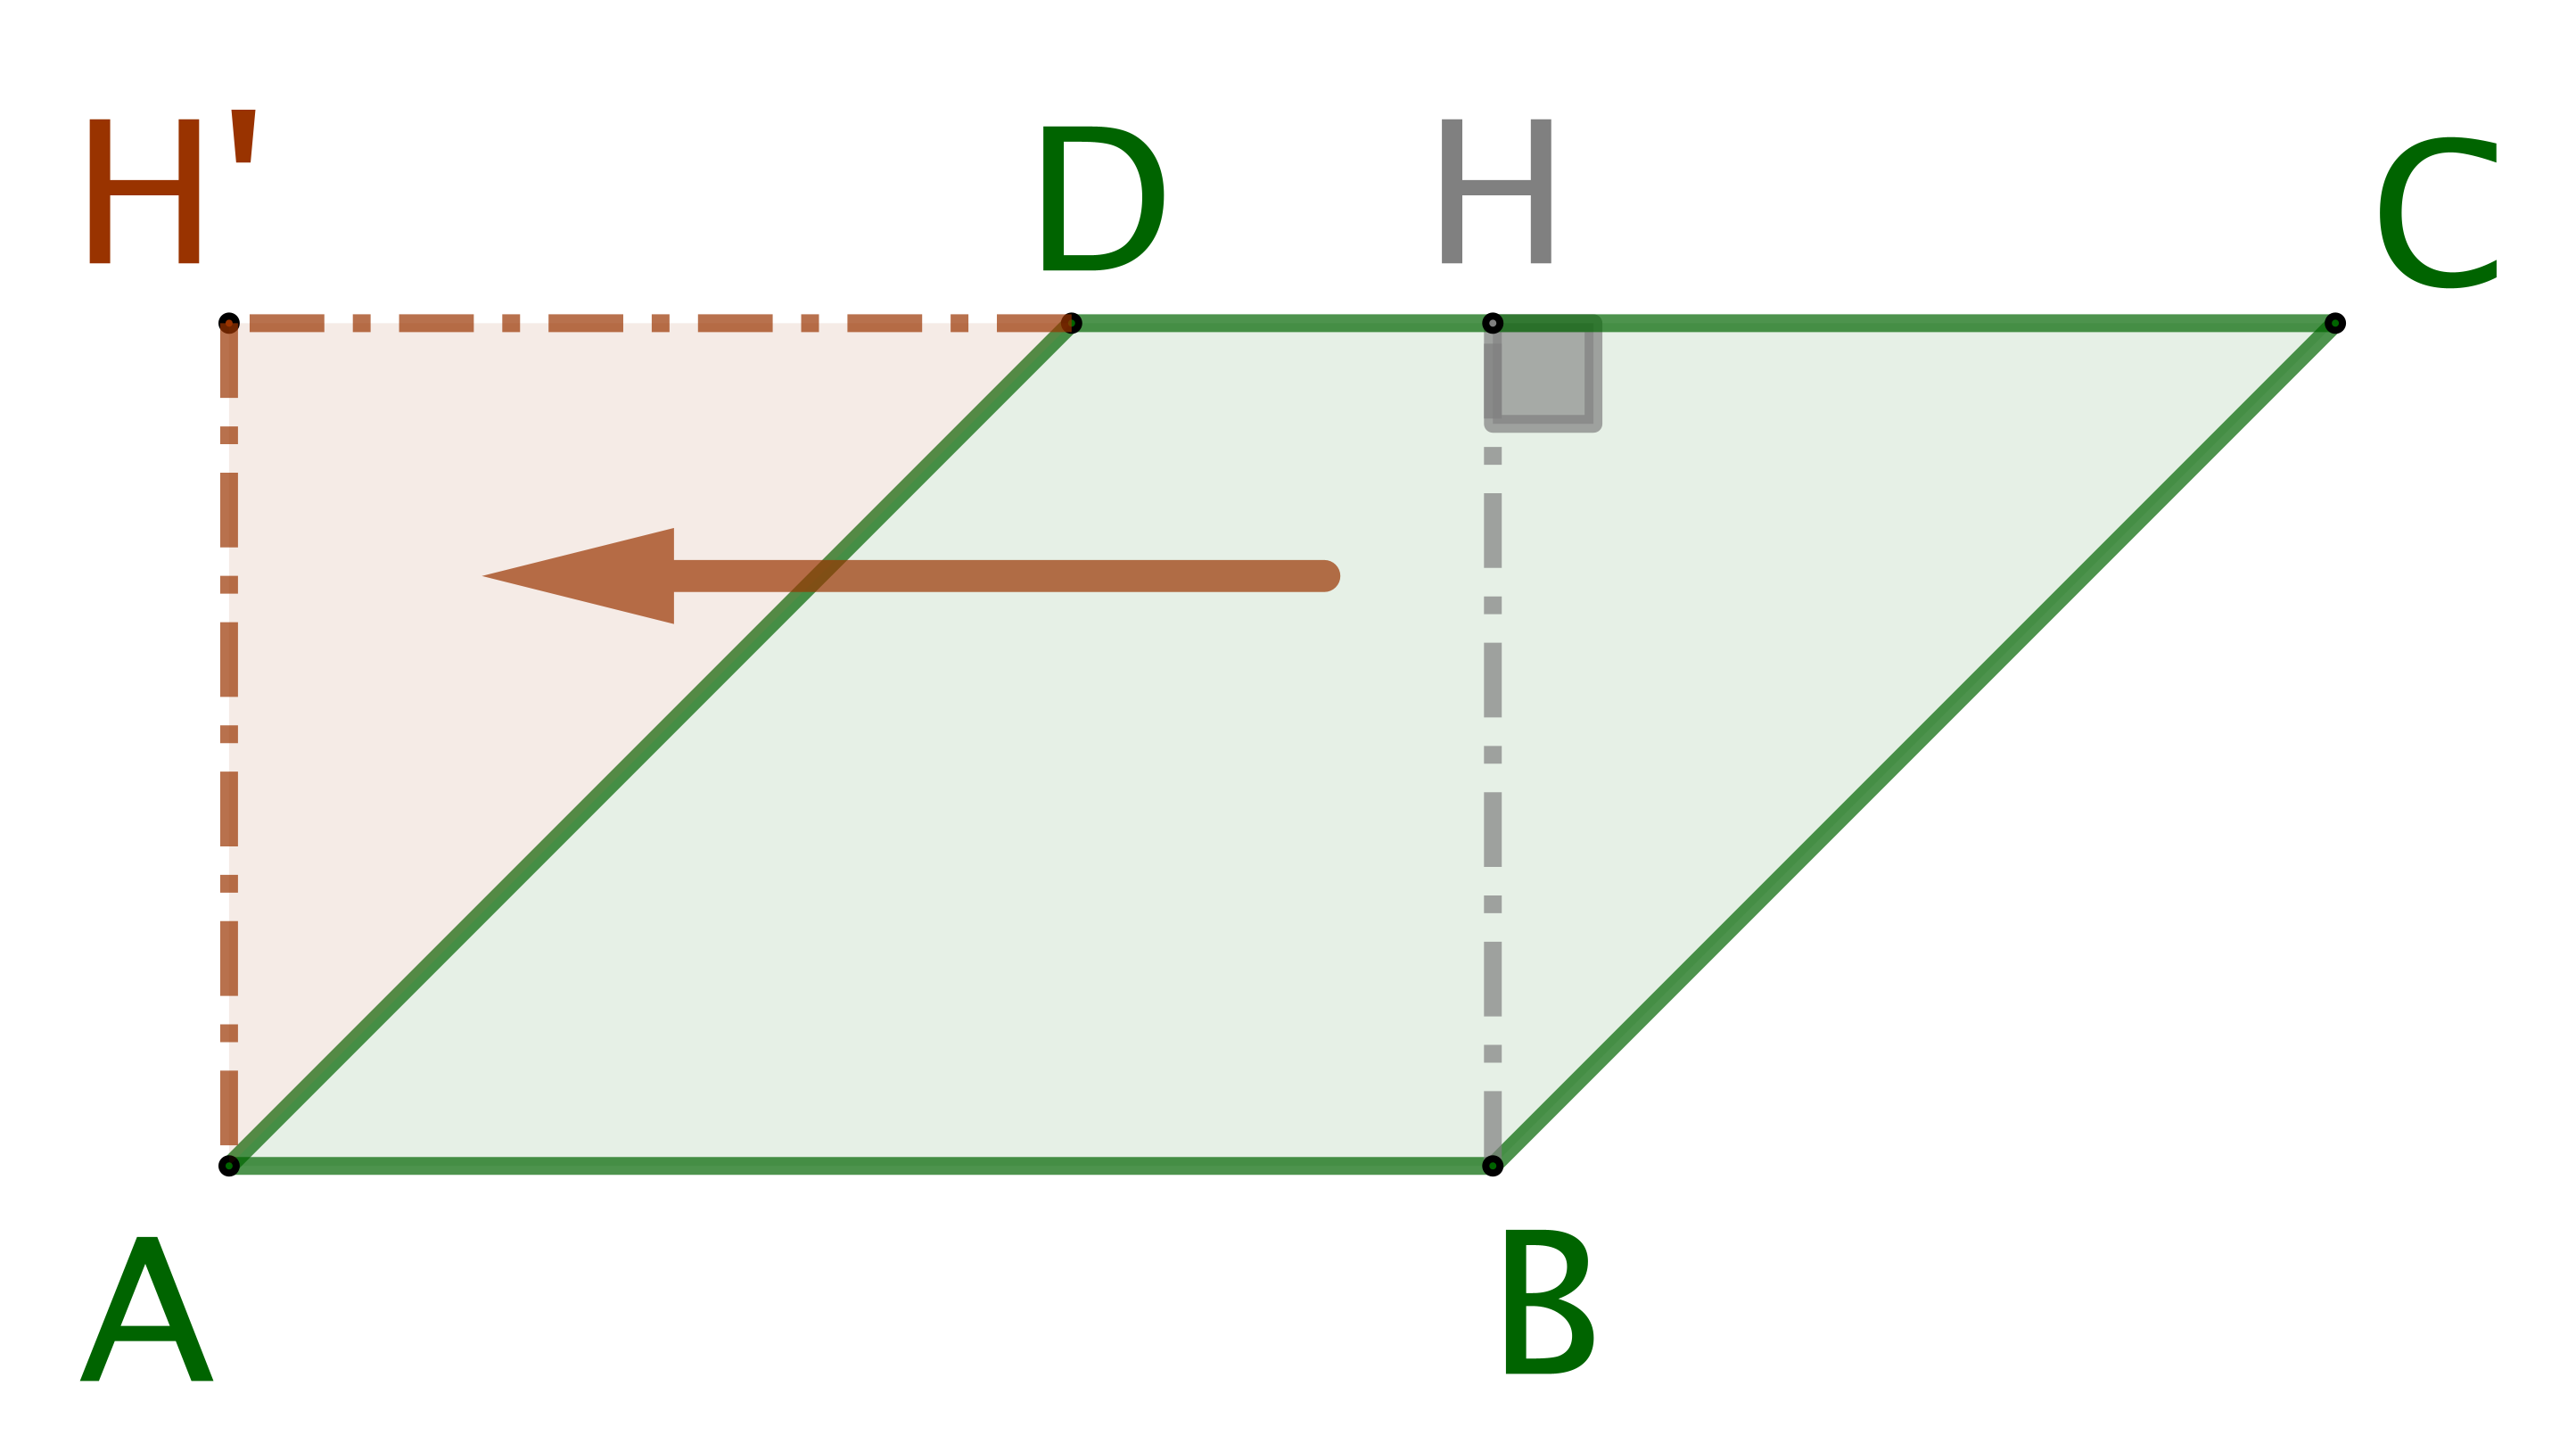
\includegraphics[scale=.4]{content/parallelogram/para-2-rect.png}
	\end{center}
	
	Via une homothétie de rapport $r = \frac{\perim{ABCD}}{\perim{ABHH^{\,\prime}}} \geq 1$, nous obtenons un rectangle 
	de périmètre égal à $p$,
	et d'aire supérieure ou égale à $\area{ABCD}$, 
	avec égalité uniquement si $ABCD$ est un rectangle.
	Nous revenons à la situation du fait \ref{iso-rect} qui permet de conclure très facilement.
\end{proof}


% ----------------------- %


\begin{remark}
	Une méthode analytique devient pénible ici, car il faut, par exemple, prendre en compte l'angle au sommet $A$ du parallélogramme. L'auteur préfère battre en retraite en clôturant cette remarque ici.
%	\footnote{
%		Et oui, l'auteur est un lâche.
%	}
\end{remark}

%
%
%\subsection{Le cas général}
%\begin{fact}
	Considérons tous les quadrilatères de périmètre fixé $p$. Parmi tous ces quadrilatères, celui d'aire maximale est le carré de côté $c = \num{.25} p$.
\end{fact}


\begin{proof}
	La figure suivante montre que pour tout quadrilatère $ABCD$ non convexe en $B$, et de périmètre $p$, il existe un quadrilatère convexe $AB^{\,\prime}CD$ de périmètre $p$, et tel que $\area{AB^{\,\prime}CD} \geq \area{ABCD}$.
	Notre recherche doit donc continuer dans l'ensemble des quadrilatères convexes de périmètre $p$.

	\begin{center}
		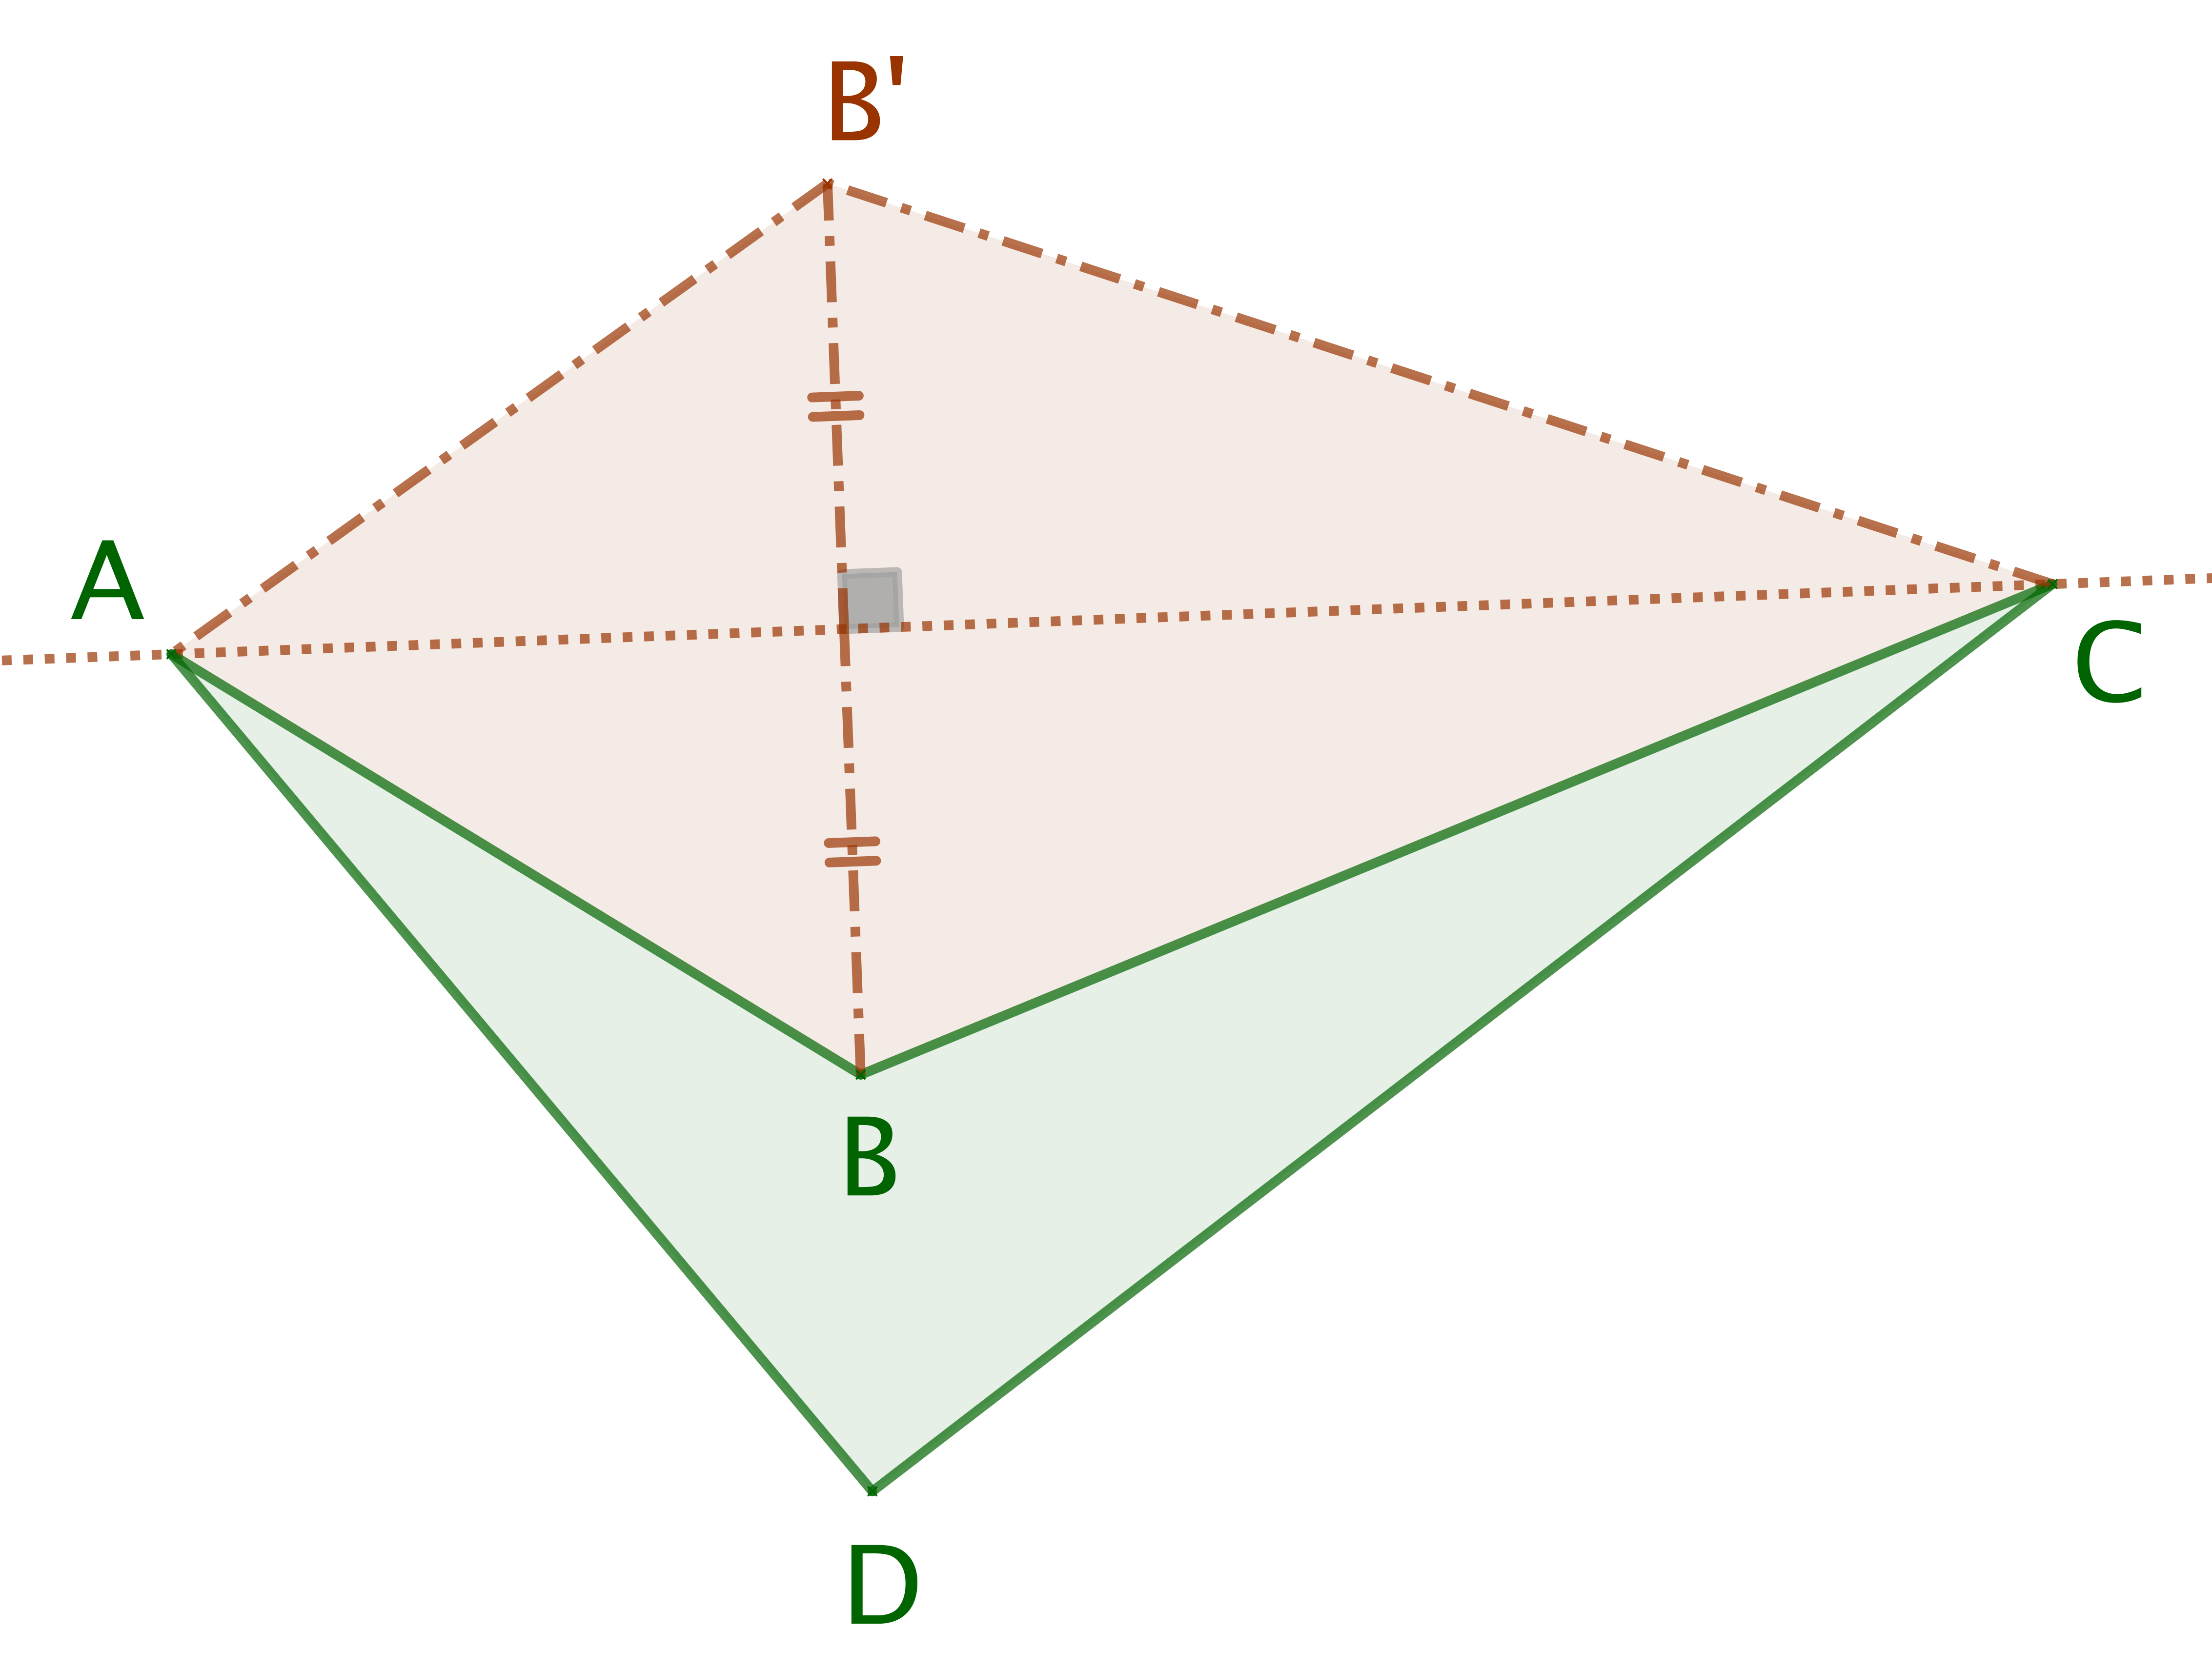
\includegraphics[scale=.4]{content/quadrilateral/quadrilateral-non-convex.png}
	\end{center}
	
	
	Comme dans la preuve du fait \ref{iso-tri-one-side-fixed}, à partir d'un quadrilatère convexe $ABCD$ de périmètre $p$, nous obtenons un quadrilatère convexe $AB^{\,\prime}CD$ de périmètre $p$,%
	\footnote{
		Noter que
		$\perim{AB^{\,\prime}CD} = \perim{AB^{\,\prime}C} + \perim{ACD} - 2 AC$.
	}
	et tel que $AB^{\,\prime} = B^{\,\prime}C$ et $\area{AB^{\,\prime}CD} \geq \area{ABCD}$ comme le montre la figure ci-après. 

	\begin{center}
		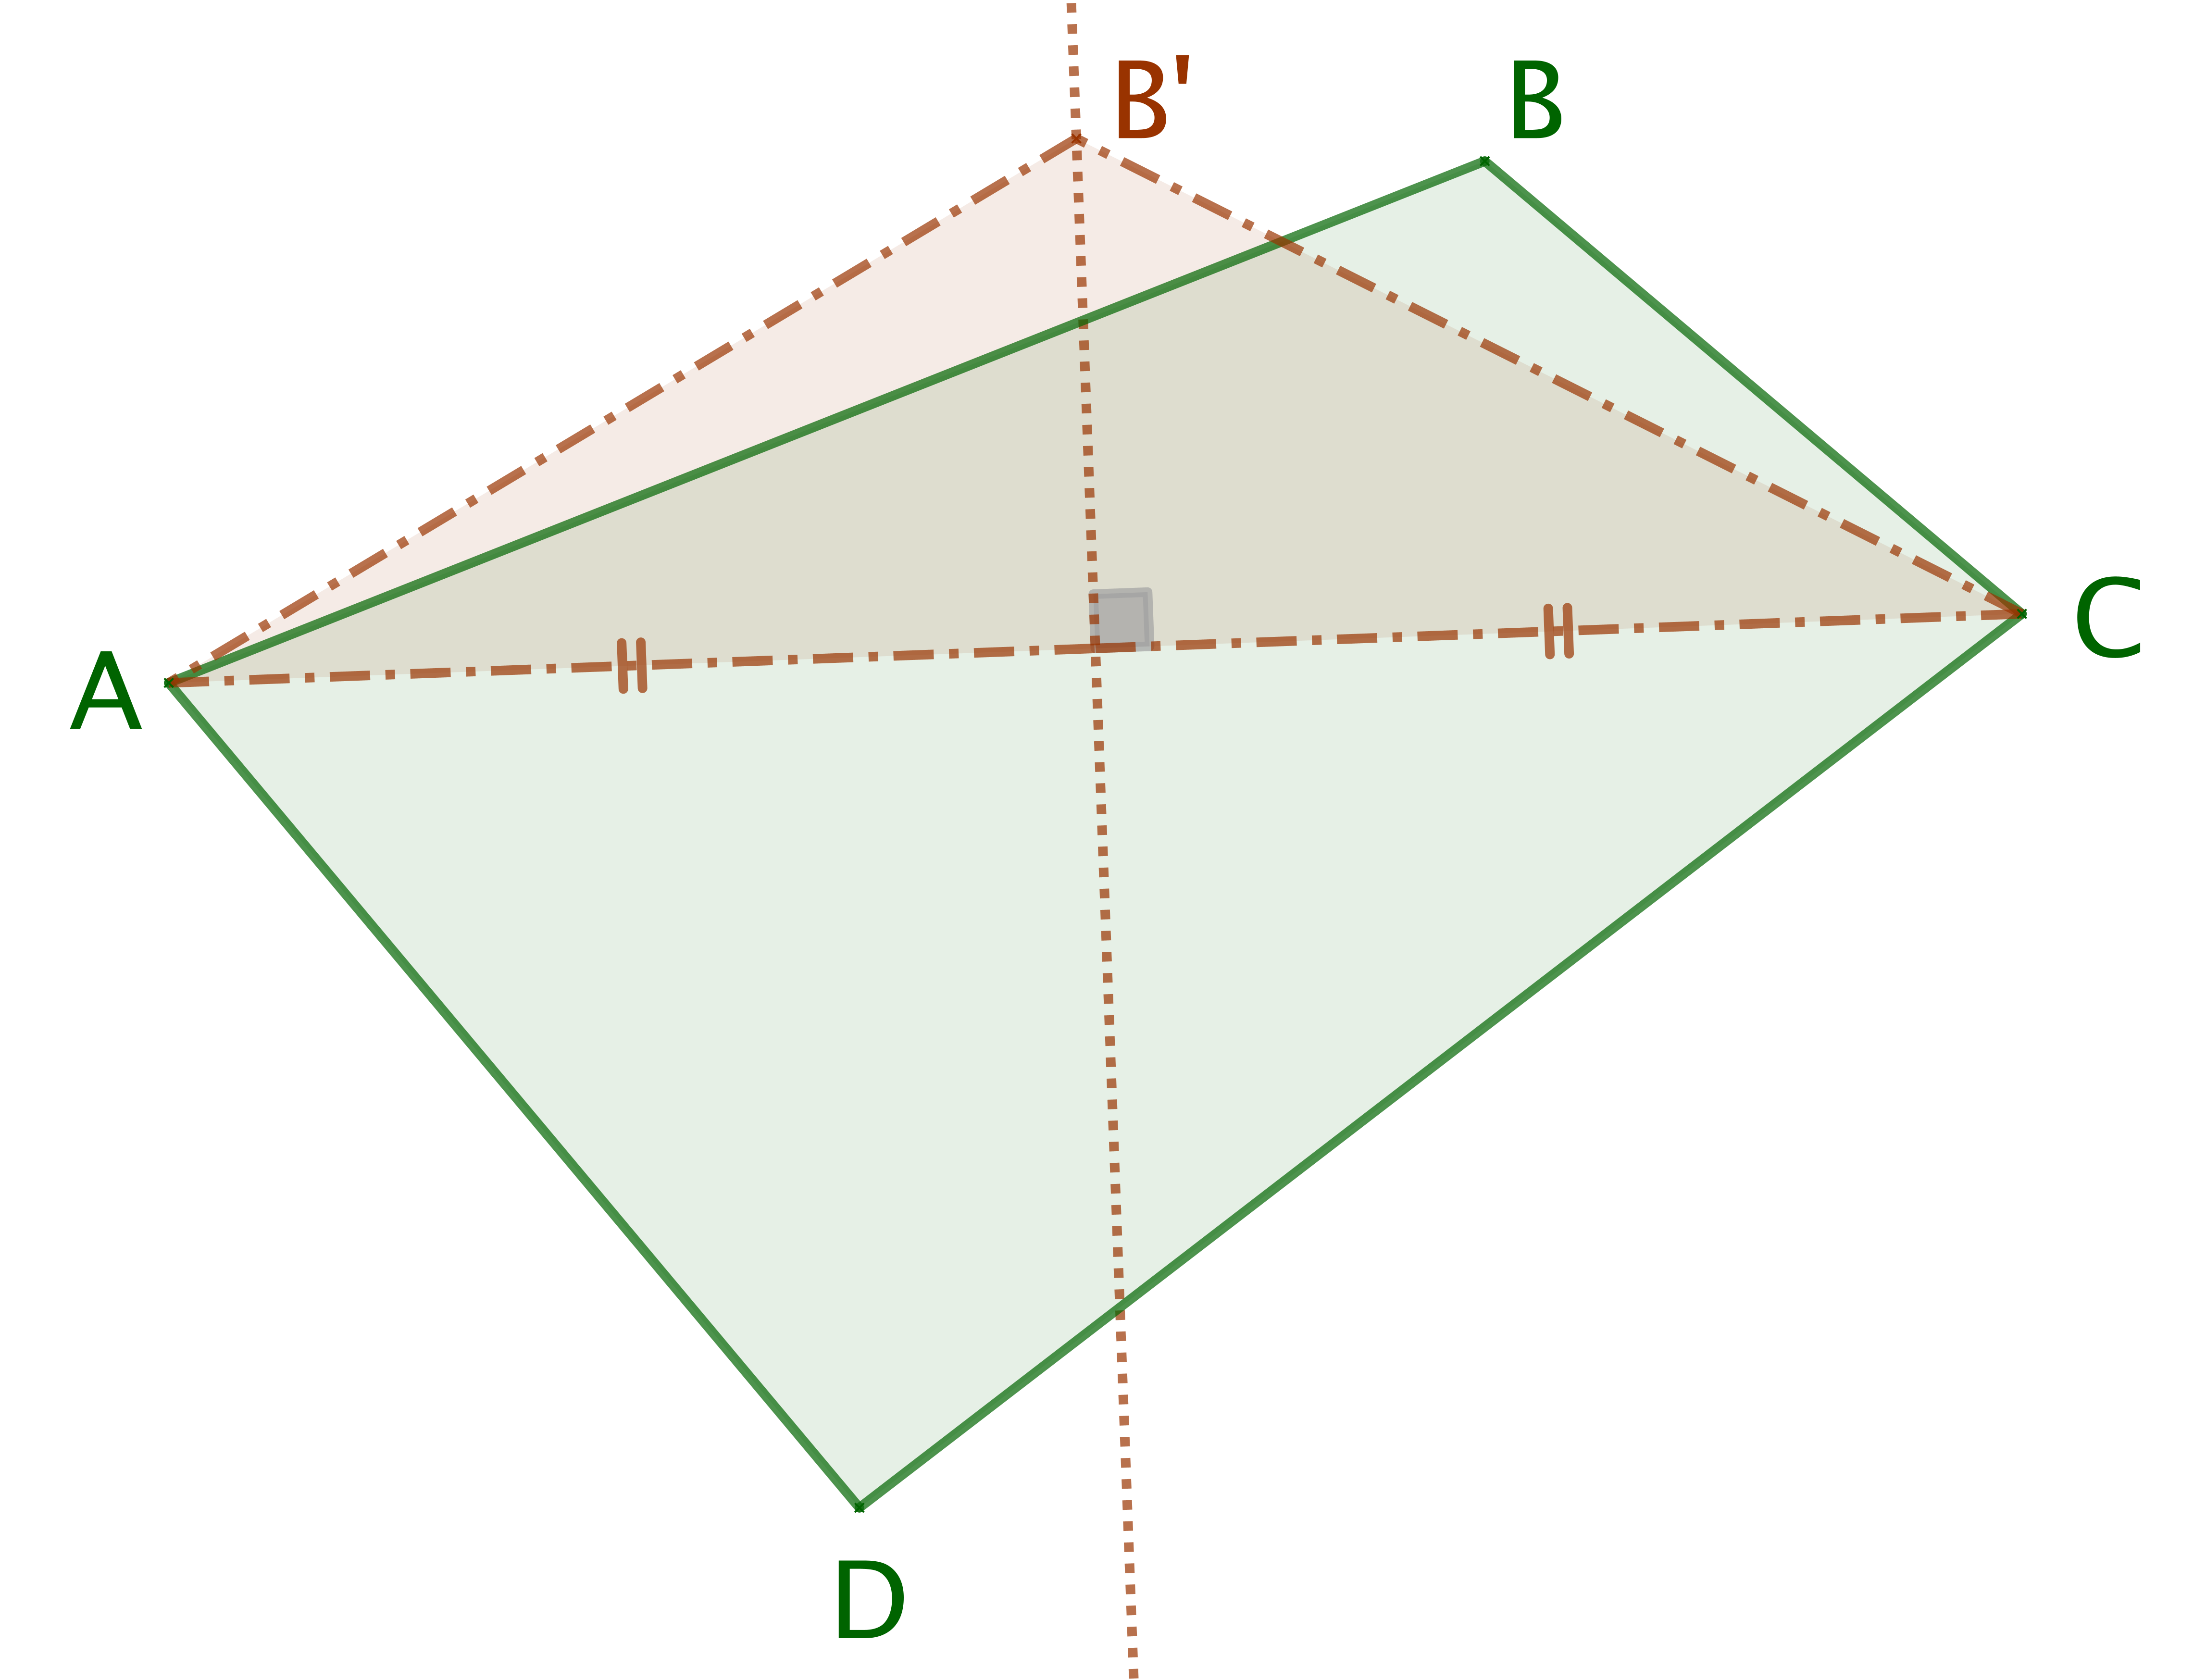
\includegraphics[scale=.4]{content/quadrilateral/quadrilateral-convex-gene.png}
	\end{center}
	
	
	La méthode précédente appliquée au sommet $D$ donne un cerf-volant $ABCD$ de périmètre $p$, et tel que $AB = BC$ et $AD = DC$, voir ci-dessous. 
	Cette même méthode avec les sommets $A$ et $C$ fournit un losange $A^{\,\prime}BC^{\,\prime}D$ de périmètre $p$, et tel que $\area{A^{\,\prime}BC^{\,\prime}D} \geq \area{ABCD}$.
	%
	En effet, nous avons
	$p = 2(AB + AD)$
	et
	$\perim{A^{\,\prime}BD} = \perim{ABD}$,
	donc
	$A^{\,\prime}B = A^{\,\prime}D = \num{.25} p$,
	et de même, nous obtenons
	$C^{\,\prime}B = C^{\,\prime}D = \num{.25} p$.

	\begin{center}
		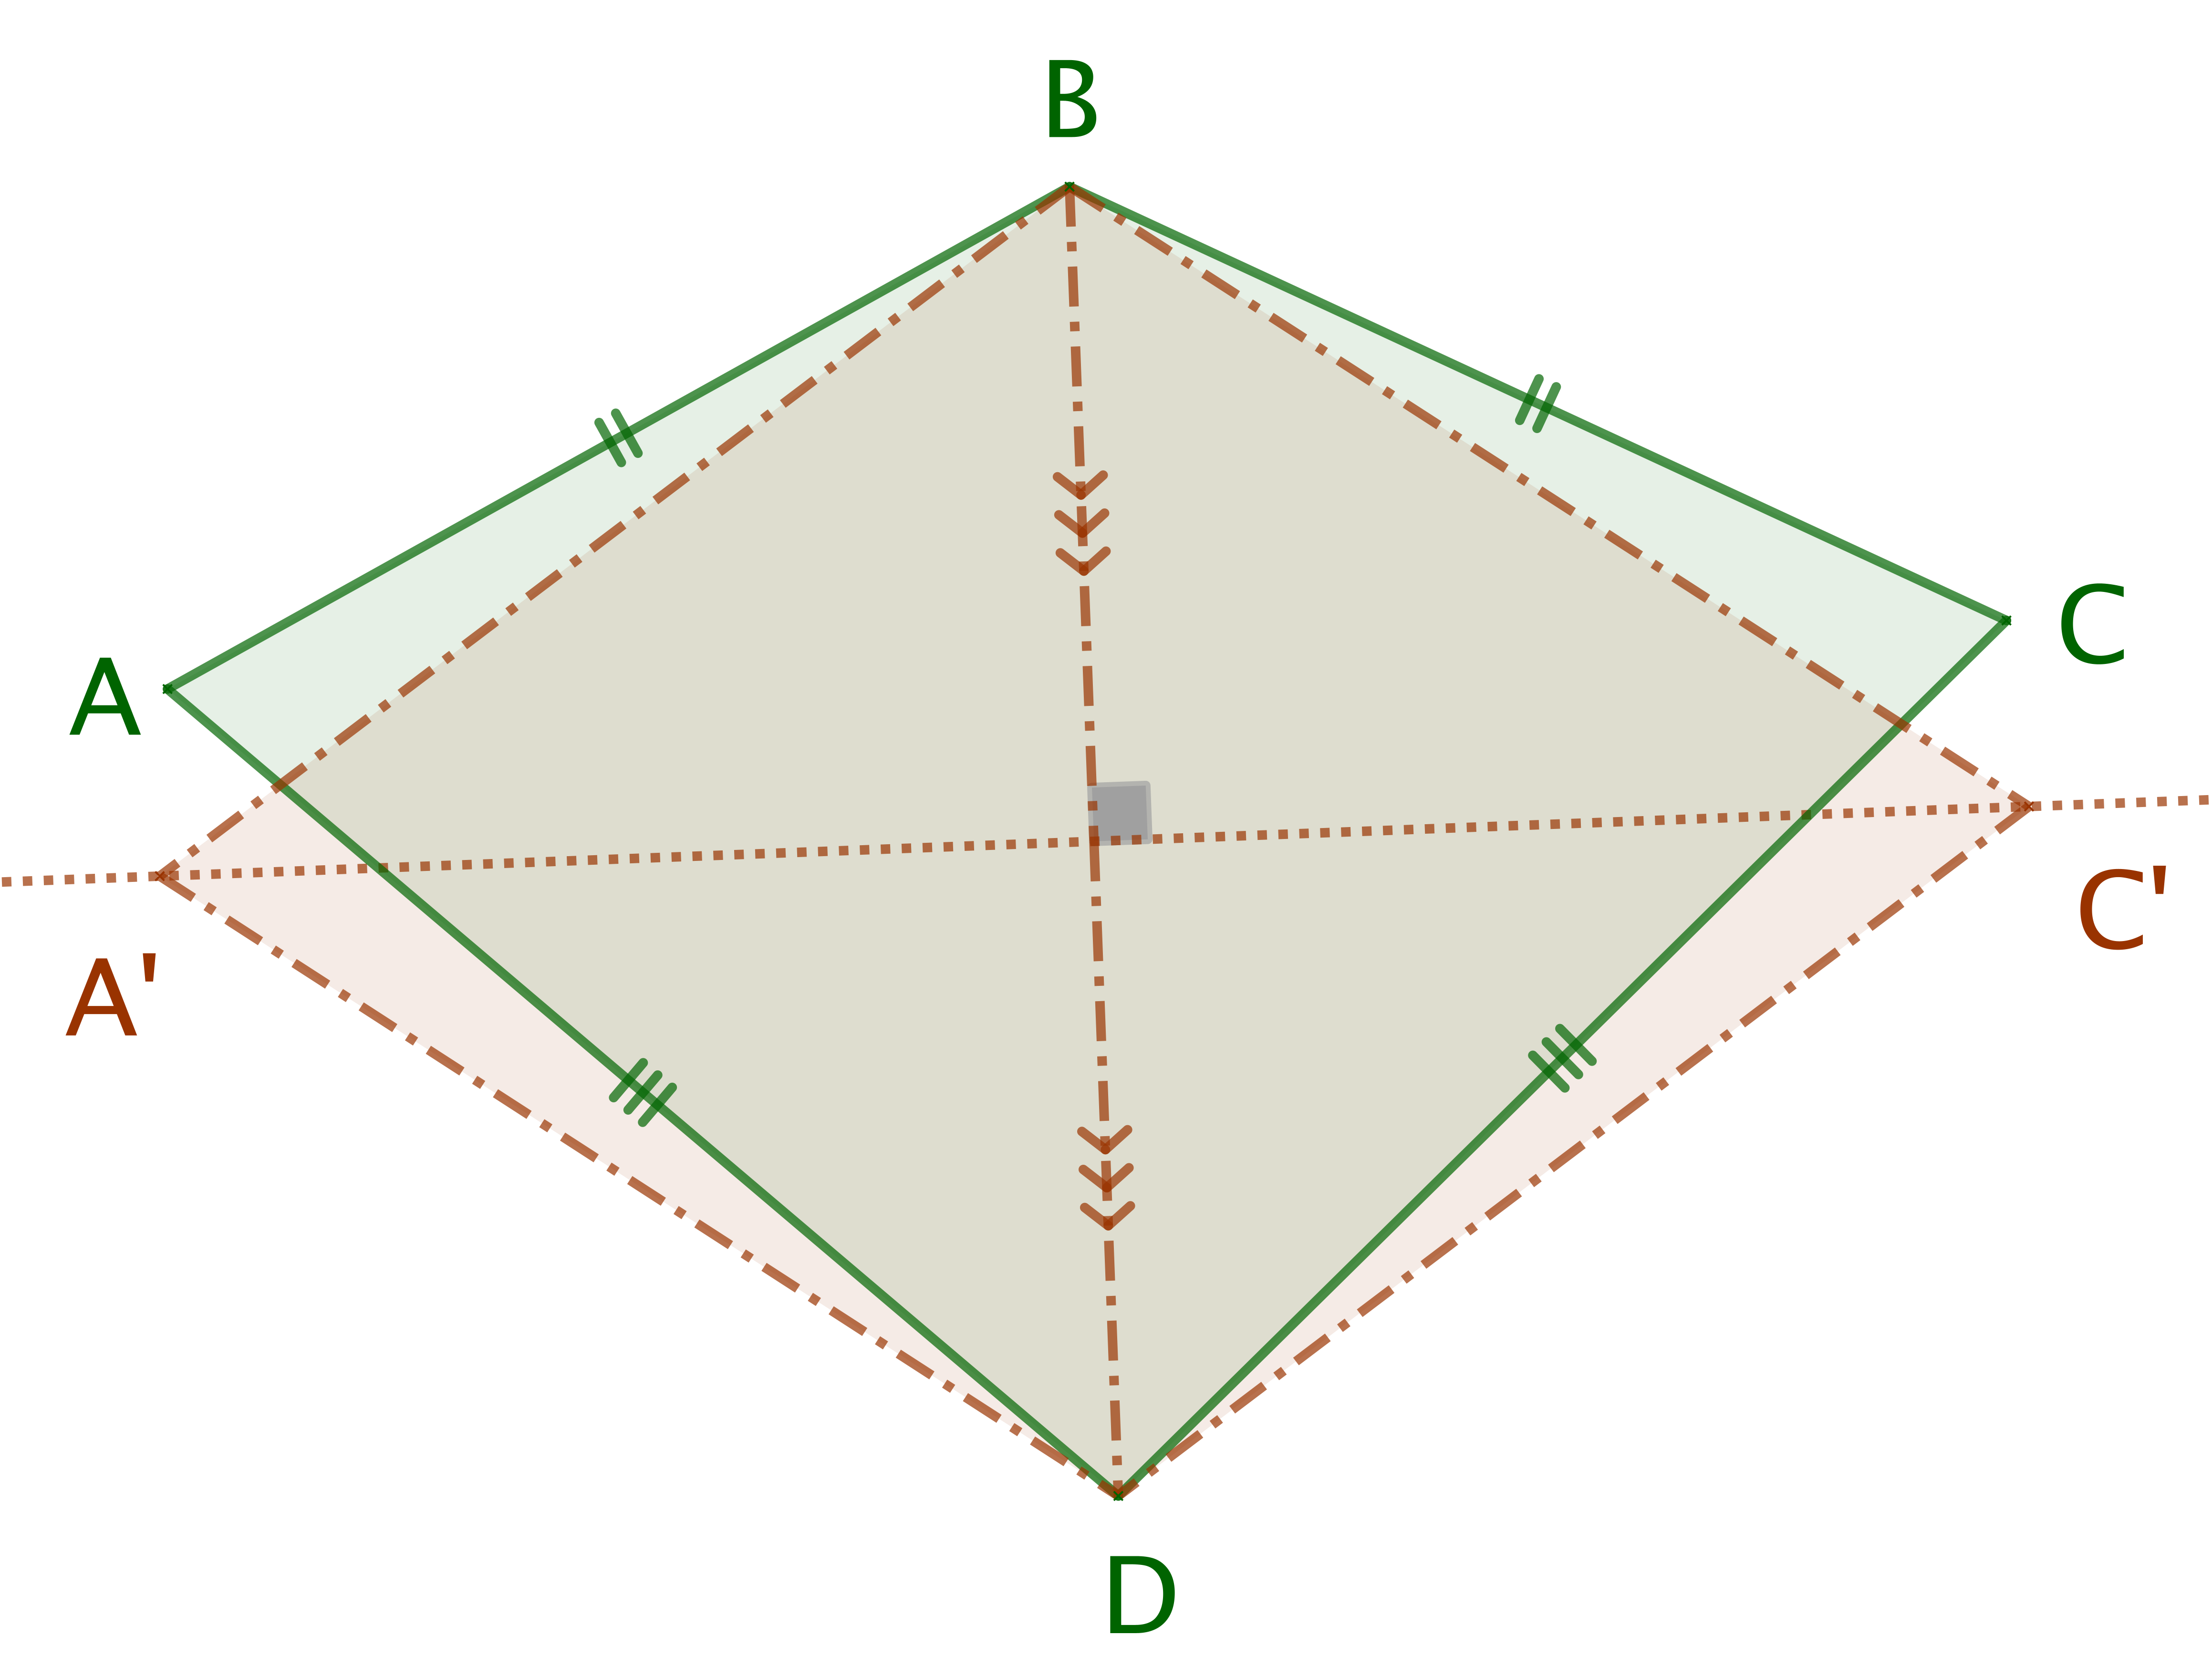
\includegraphics[scale=.4]{content/quadrilateral/quadrilateral-convex-isopaire.png}
	\end{center}
	
	
	Pour conclure, il suffit d'appliquer le fait \ref{iso-para}, puisque tout losange est un parallélogramme. Que la géométrie est belle!
\end{proof}


%
%
%% ------------- %   
%
%
%\section{Les polygones}
%
%\subsection{Où allons-nous?}
%Le passage aux polygones à $n$ côtés, pour $n \geq 5$, va mêler analyse et géométrie: nous utiliserons les notions de compacité, de continuité, de convexité \focus{élargie} et de déterminant.


\begin{tcolorbox}
    \itshape\small
    L'approche proposée n'est pas originale dans sa globalité: voir, par exemple, "Isopérimètres en toute simplicité" de Lion Georges dans Bulletin de l'APMEP. N° 496., page 566-578.%
    \footnote{
        L'auteur du présent texte n'a eu connaissance du document de Lion Georges, qu'une fois son modeste travail fini.
    }
    Par contre, vous trouverez ici une approche la plus simple possible, et sans trous logiques.
\end{tcolorbox}

%
%
%\subsection{Condition nécessaire}   
%Le fait important que nous allons établir, le fait \ref{nece-cond}, impliquera que si un \ngone\ maximise son aire à périmètre fixé, alors il doit être régulier.


% ----------------------- %


\begin{fact} \label{conv-poly}
	Si un \ngone\ $\setproba{P}$ n'est pas convexe, alors on peut construire un \ngone\ convexe $\setproba{P}^{\,\prime}$ tel que 
	$\perim{\setproba{P}^{\,\prime}} = \perim{\setproba{P}}$ 
	et 
	$\area{\setproba{P}^{\,\prime}} > \area{\setproba{P}}$.
\end{fact}


\begin{proof}
	Ici, il ne faut pas être expéditif en indiquant que la preuve du fait \ref{quadri} se généralise sans aucun souci.
	En effet, avec $n > 4$, nous pouvons avoir plusieurs points de non-convexité, et les éliminer comme nous l'avons fait pour le quadrilatère n'est pas immédiat:
	dans la figure suivante, l'élimination des deux points de non convexité $G$ et $E$ de l'heptagone $ABCDEFG$ nous amène à un nouvel heptagone $ABCDE^{\,\prime}FG^{\,\prime}$ ayant lui aussi deux points de non-convexité $F$ et $D$!
	Donc, rien n'empêche, a priori, d'avoir une suite de constructions n'aboutissant jamais à un heptagone convexe
	de même périmètre que celui de $ABCDEFG$, et d'aire strictement supérieure à celle de $ABCDEFG$.%
	\footnote{
		L'auteur est convaincu que le procédé aboutira en un nombre fini d'étapes à un polygone convexe, mais il ne l'a pas démontré pour le moment (un raisonnement sur les angles aux sommets devraient permettre de valider une telle conjecture).
	}

	\begin{center}
		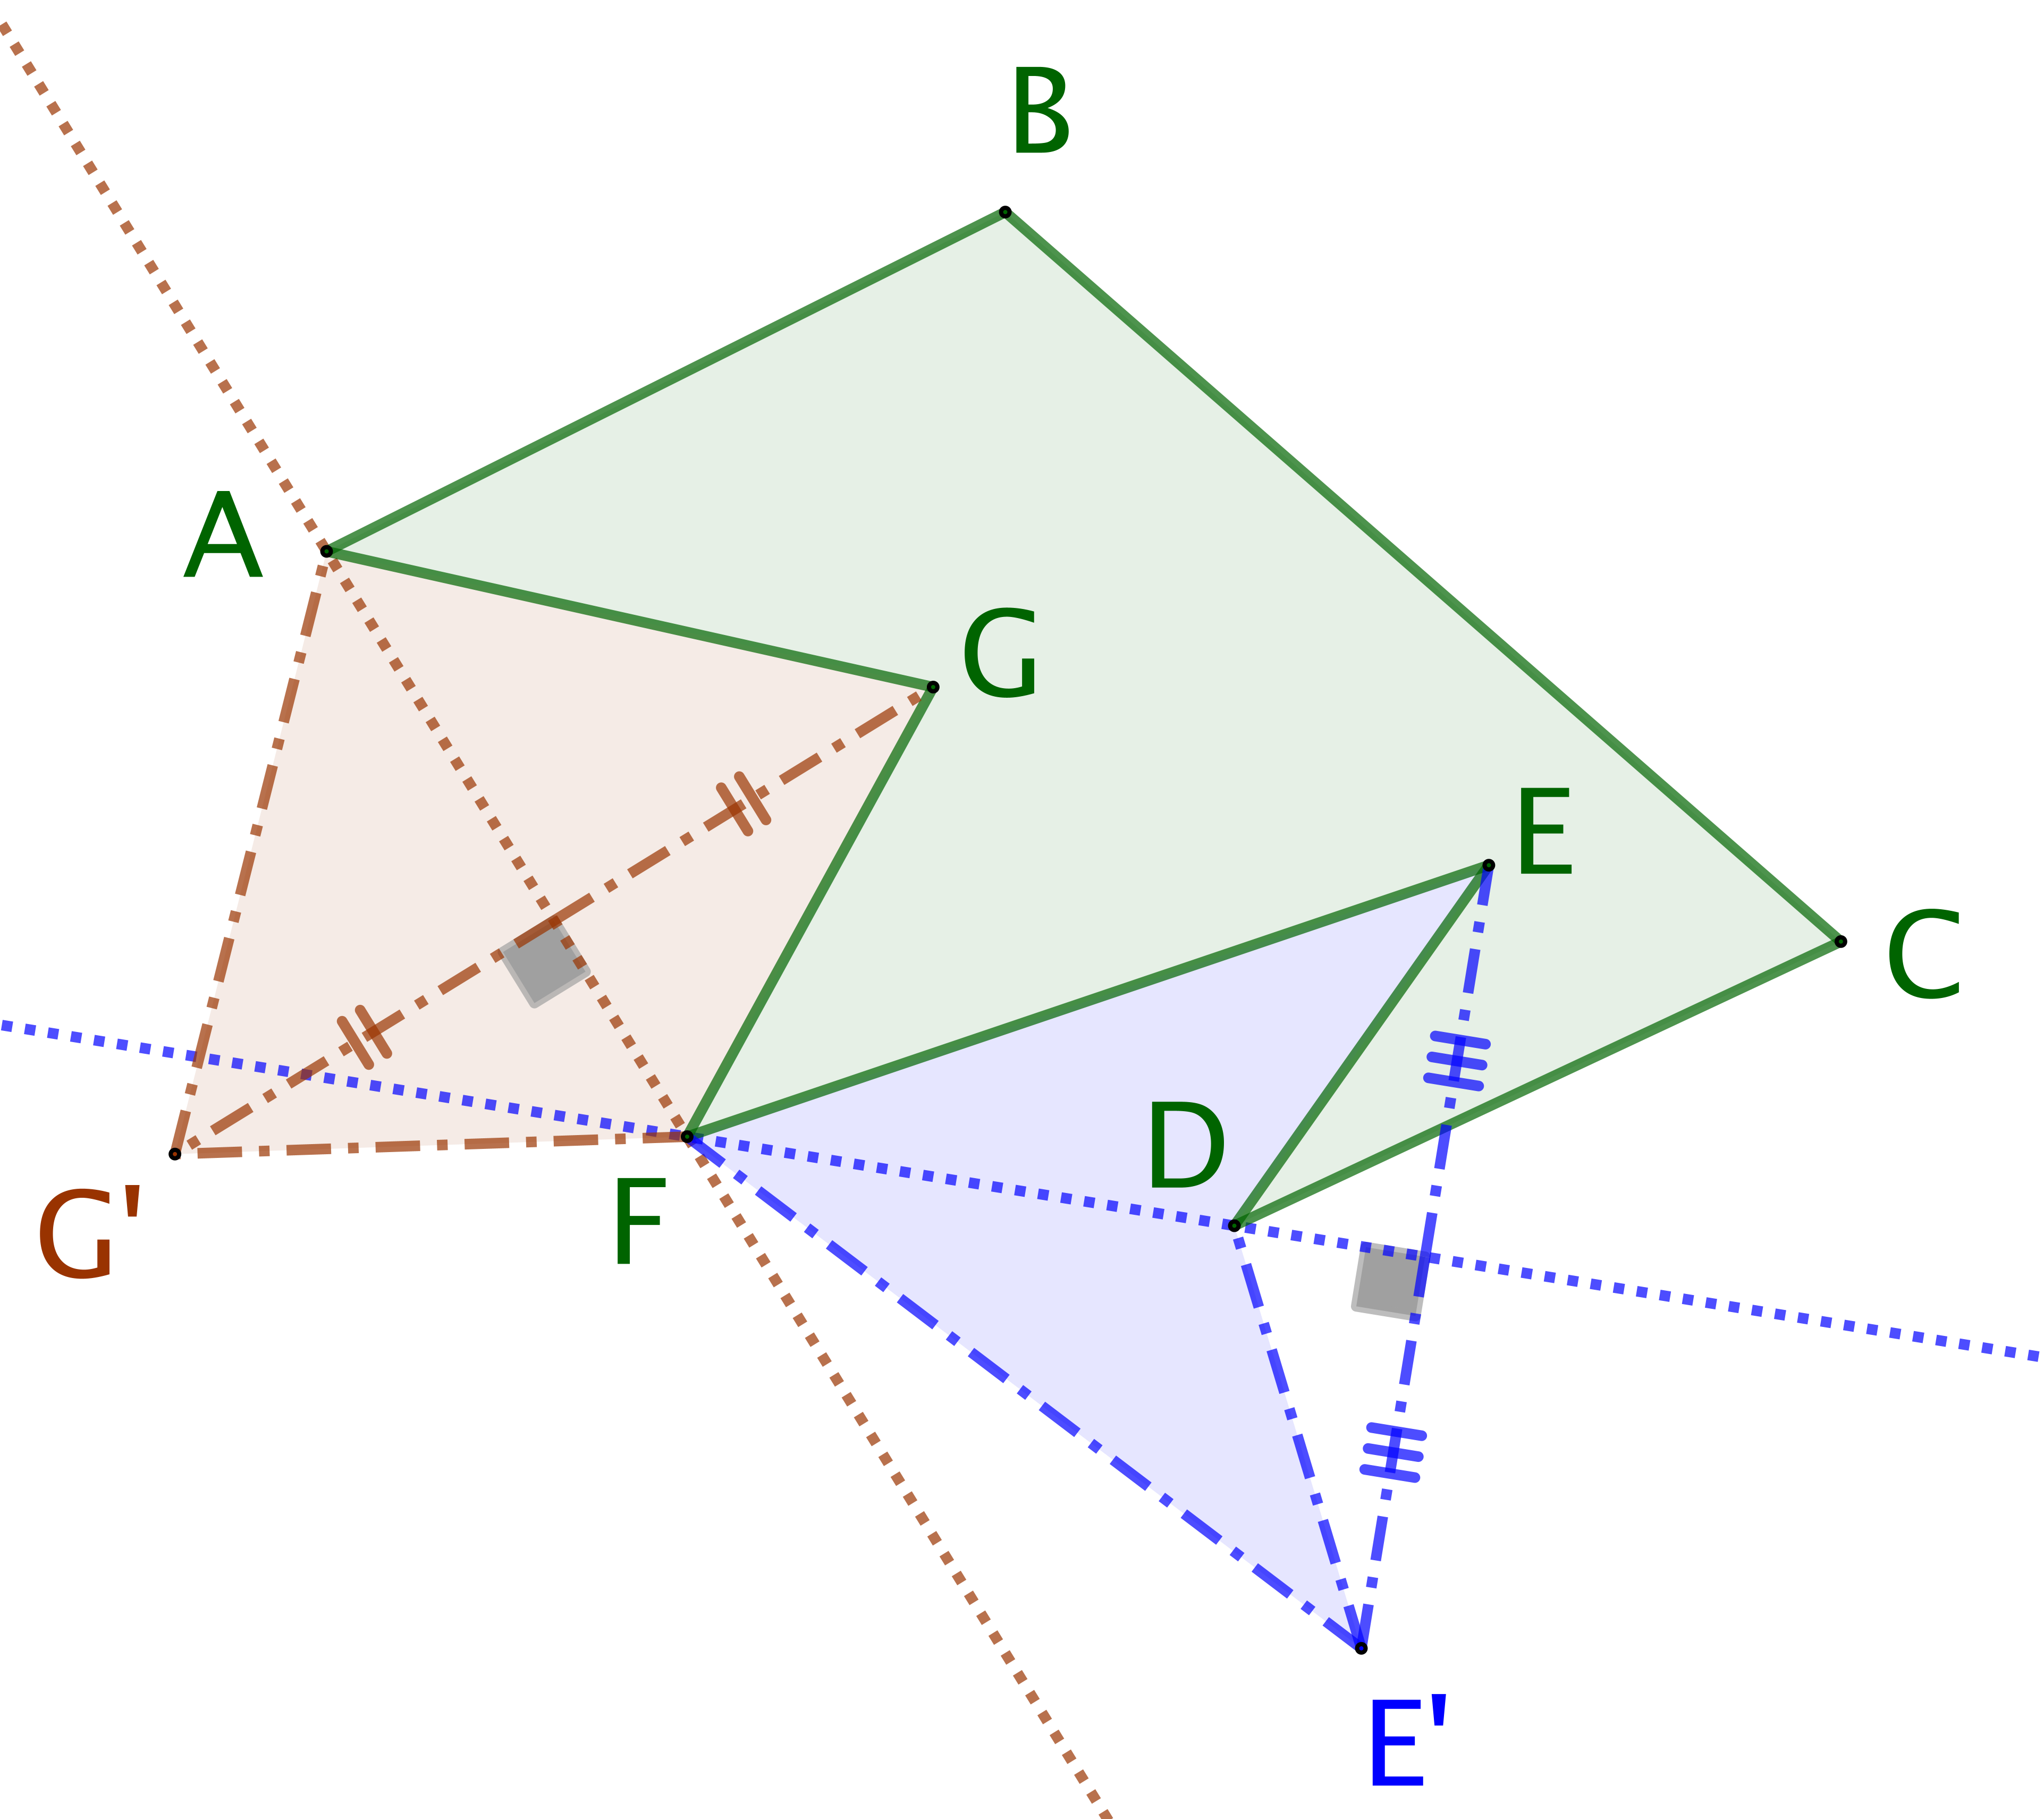
\includegraphics[scale=.4]{content/polygon/necessary-cond/non-convex-trap.png}
	\end{center}
	

	On peut aussi perdre des côtés lors de la construction comme dans l'exemple suivant où $C$, $D$ et $E^{\,\prime}$ sont alignés. Nous allons voir juste après que ce problème n'en est pas un.

	\begin{center}
		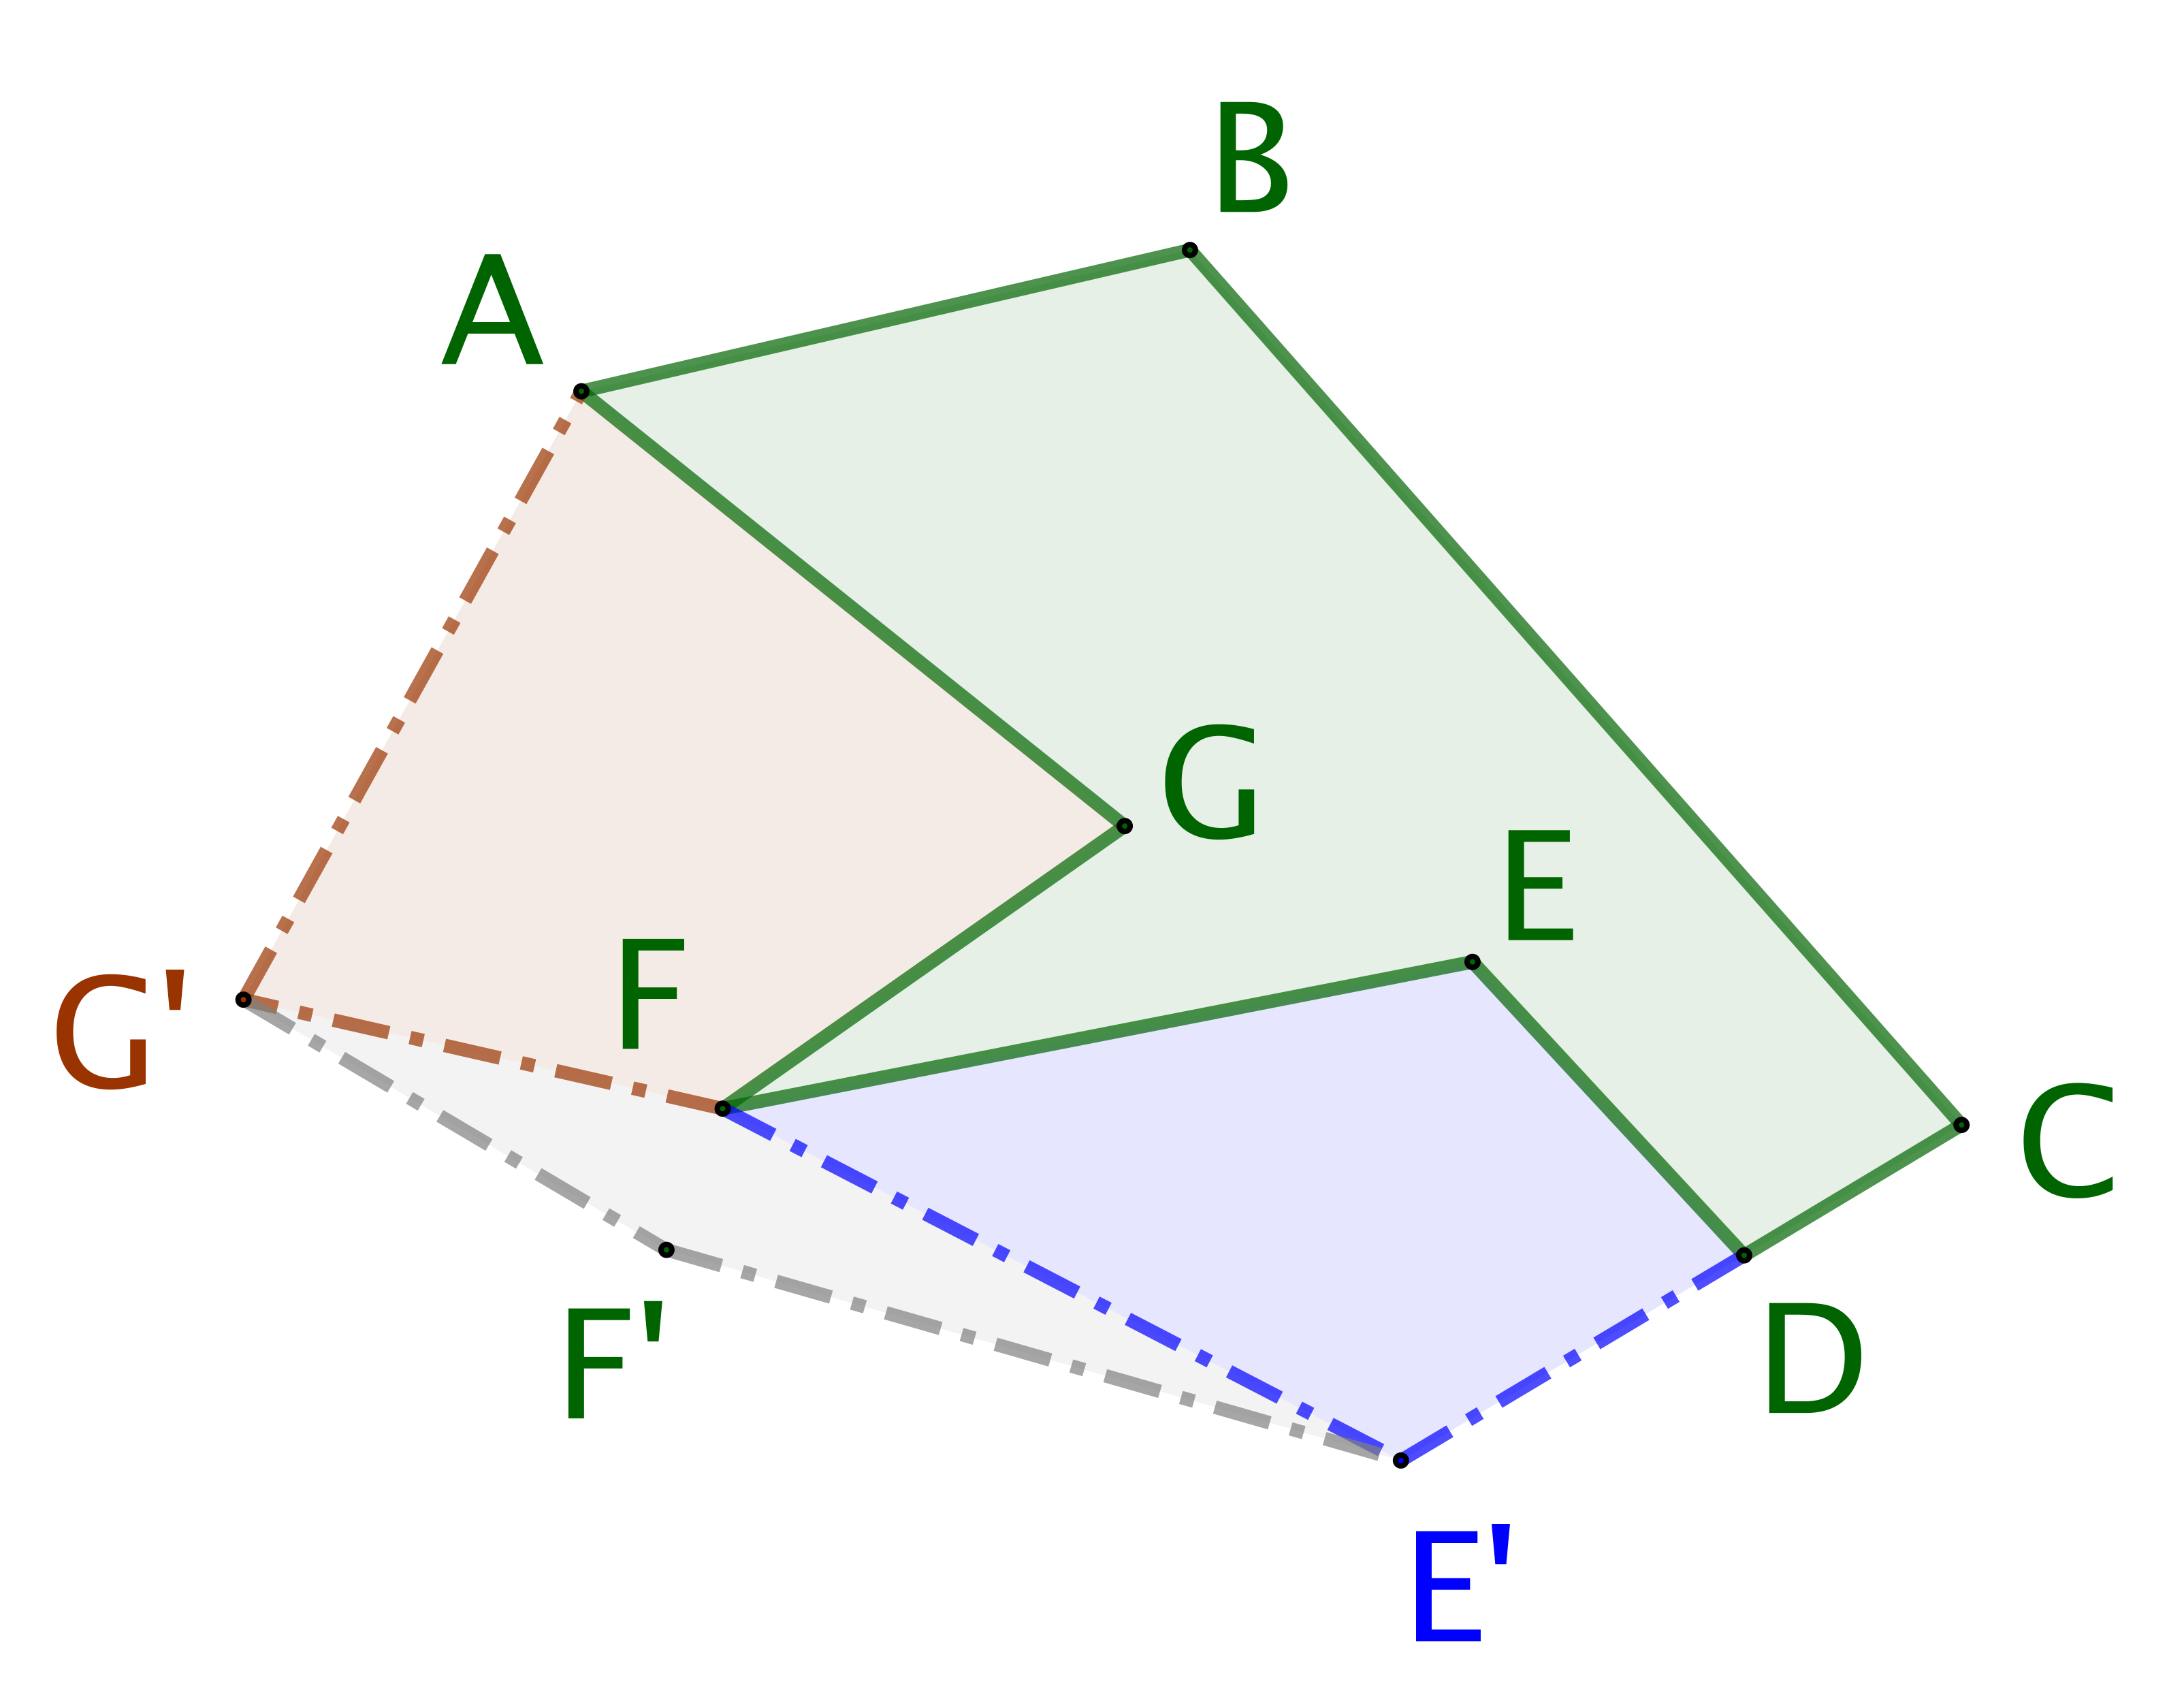
\includegraphics[scale=.4]{content/polygon/necessary-cond/non-convex-bad.png}
	\end{center}


	Laissons de côté la construction précédente pour nous concentrer sur la classique enveloppe convexe%
	\footnote{
		C'est le plus petit polygone convexe \og \emph{contenant} \fg\ le \ngone\ considéré, où \og \emph{petit} \fg\ est relatif à l'inclusion.
	}
	du \ngone\ de départ.
	Par exemple, l'ennéagone $ABCDEFGHI$ non convexe ci-dessous admet le pentagone $ABDEG$ pour enveloppe convexe: le périmètre diminue et l'aire augmentent strictement, c'est très utile, mais il reste à avoir le bon nombre de côtés.
	
	\begin{center}
		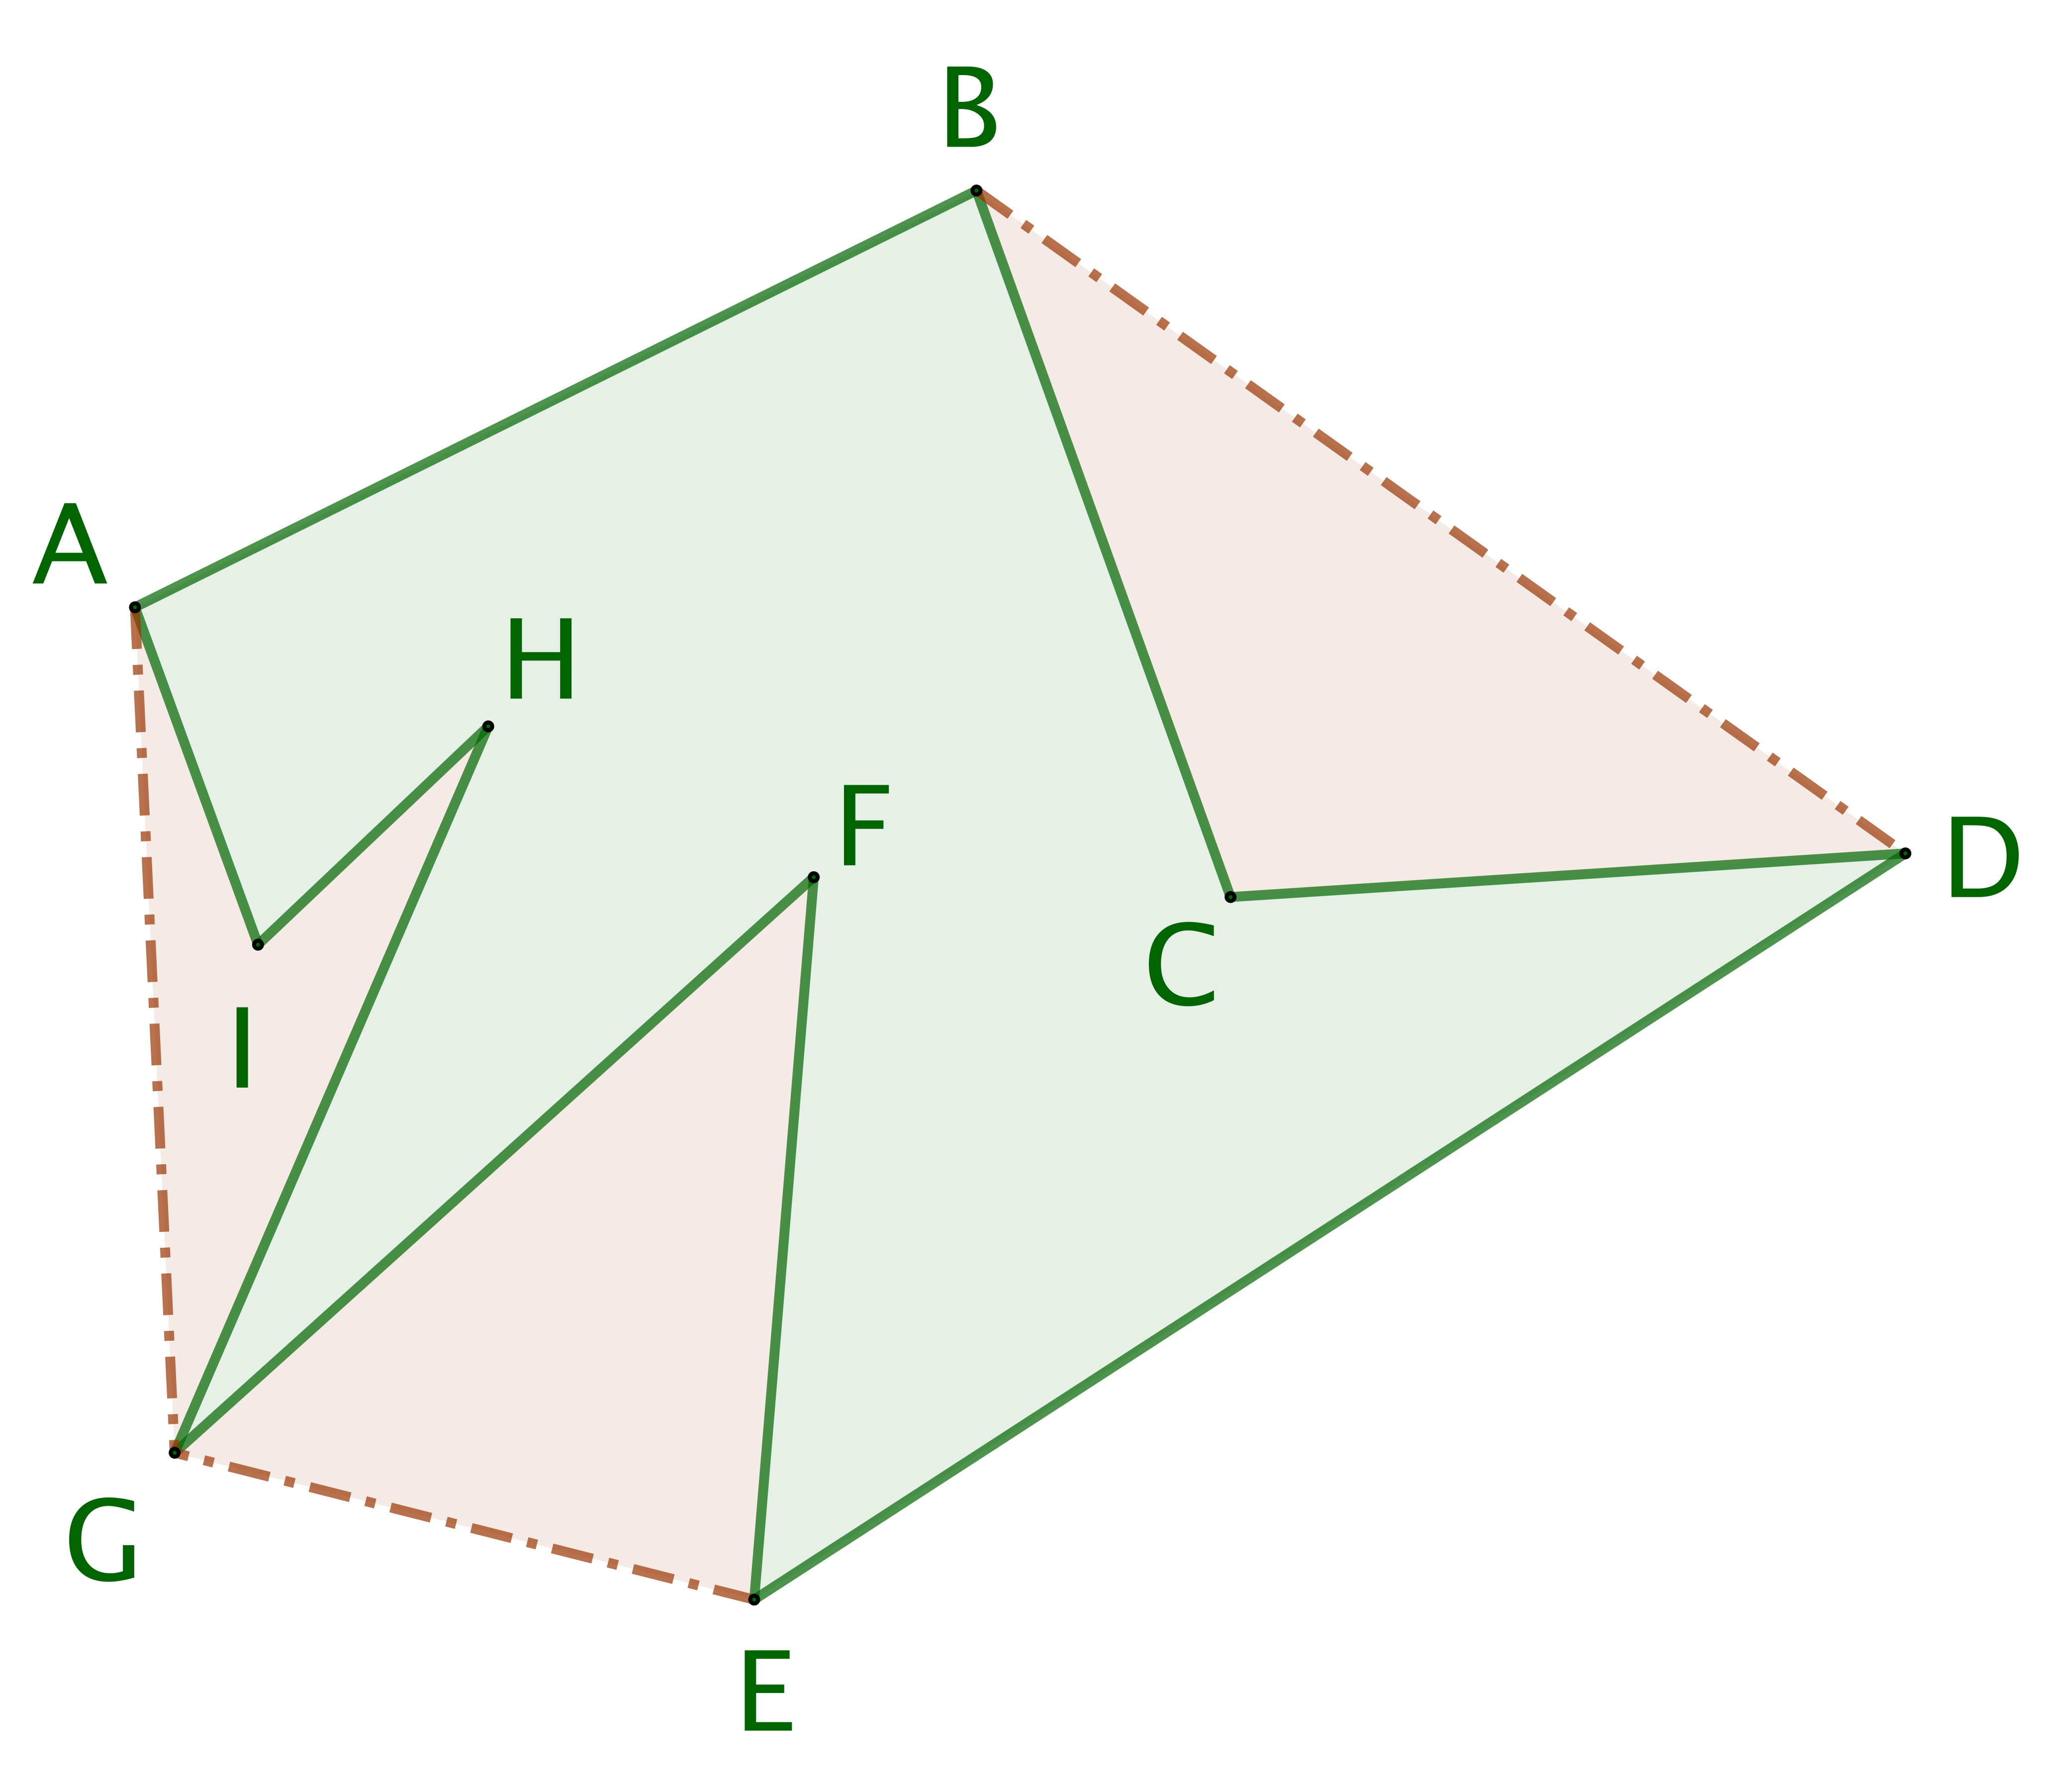
\includegraphics[scale=.4]{content/polygon/necessary-cond/convex-hull.png}
	\end{center}

	Une idée simple, que nous allons formaliser rigoureusement après, consiste à ajouter les sommets manquants suffisamment prêts des côtés de l'enveloppe convexe pour ne pas perdre la convexité, tout en gardant un périmètre inférieur strictement au périmètre initial, et une aire strictement plus grande que l'aire initiale. Si nous arrivons à faire ceci, alors une homothétie de rapport $r > 1$ nous ramènera au bon périmètre avec une aire strictement plus grande que l'aire initiale.
	La figure suivante illustre cette idée.	
	
	\begin{center}
		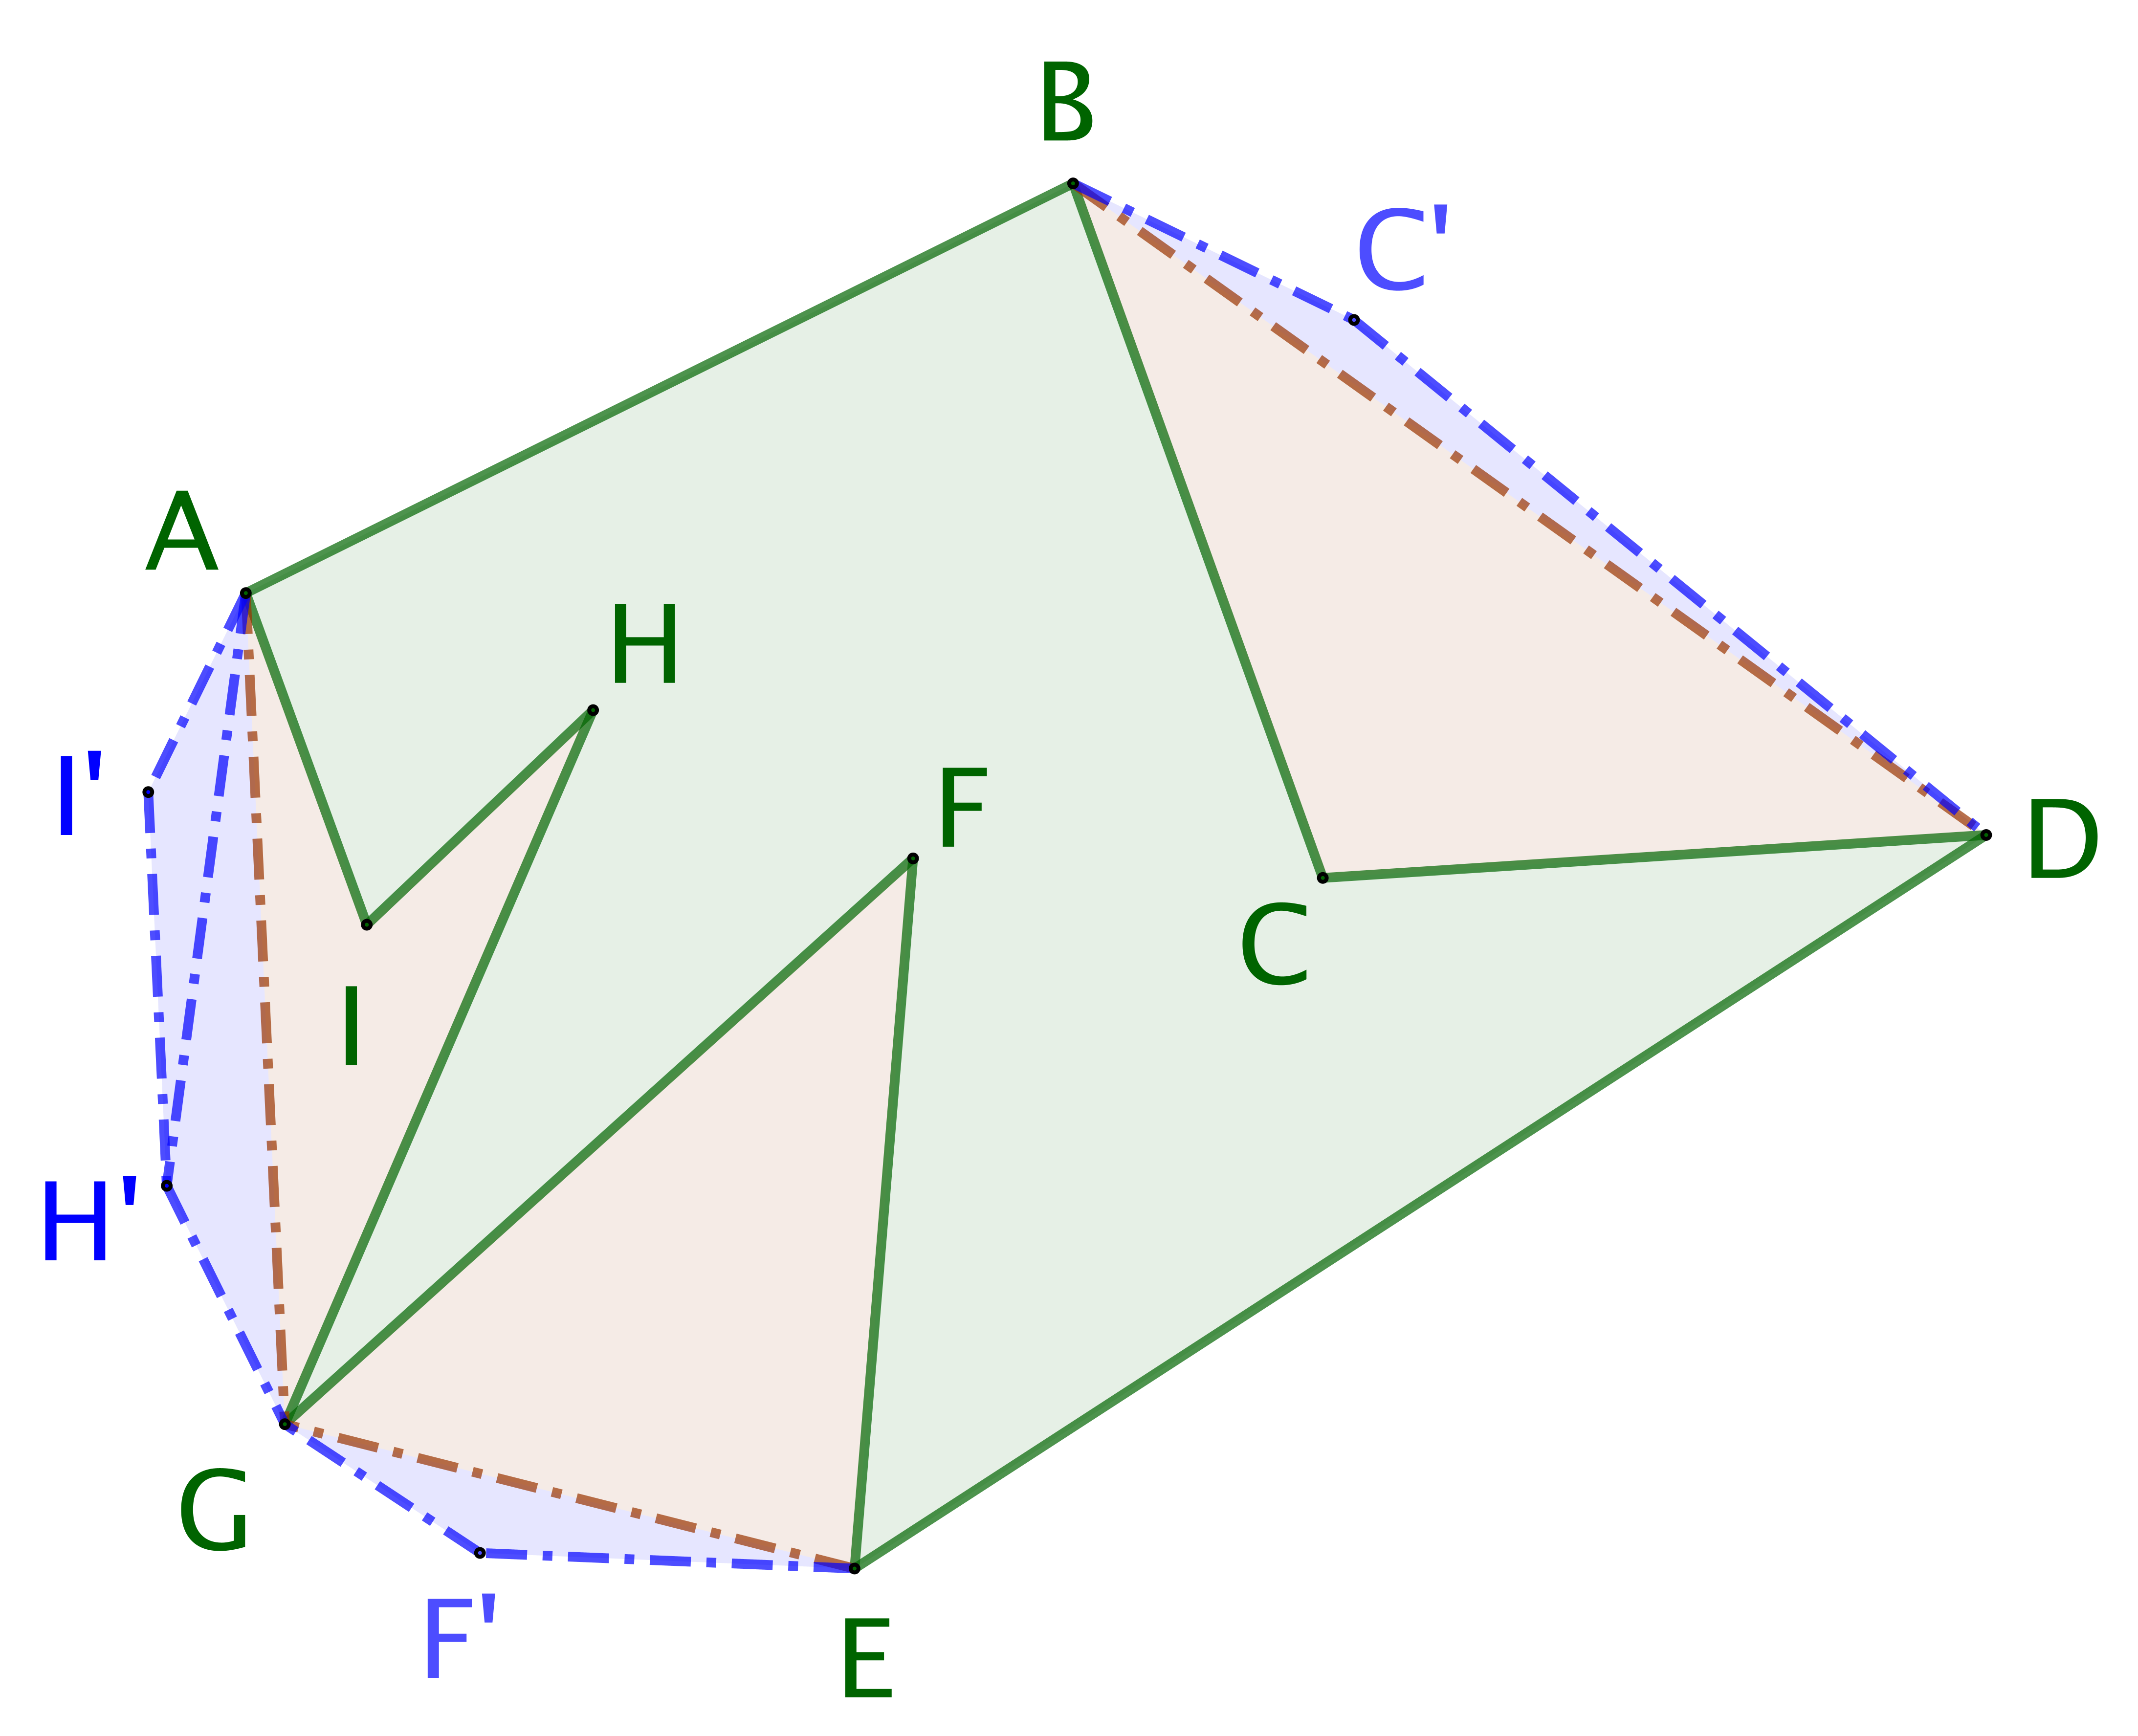
\includegraphics[scale=.4]{content/polygon/necessary-cond/convex-hull-distortion.png}
	\end{center}


	Considérons donc un \ngone\ non convexe $\setproba{P}$, donc $\setproba{P}$ possède au moins $4$ sommets.
	Son enveloppe convexe $\setproba{C}$ vérifie, par construction,
	$\perim{\setproba{C}} < \perim{\setproba{P}}$ 
	et 
	$\area{\setproba{C}} > \area{\setproba{P}}$.
	Notons $m$ le nombre de sommets en moins dans $\setproba{C}$ relativement à $\setproba{P}$ et
	$\delta = \perim{\setproba{P}} - \perim{\setproba{C}}$.
	%
	\begin{enumerate}
		\item \label{add-vertex-start}
		Si $m = 0$, il n'y a rien à faire. 

		\item Sinon, considérons $[AB]$ un côté quelconque de $\setproba{C}$.
		Les droites portées par les côtés \og \emph{autour} \fg\ de $[AB]$ \og \emph{dessinent} \fg\ une région contenant toujours un triangle $ABC$ dont l'intérieur est à l'extérieur
		\footnote{
			C'est ce que l'on appelle de la \og \emph{low poetry} \fg\,.
		}
		de $\setproba{C}$ comme dans les deux cas ci-dessous.
	%	
		\begin{multicols}{2}
			\centering

			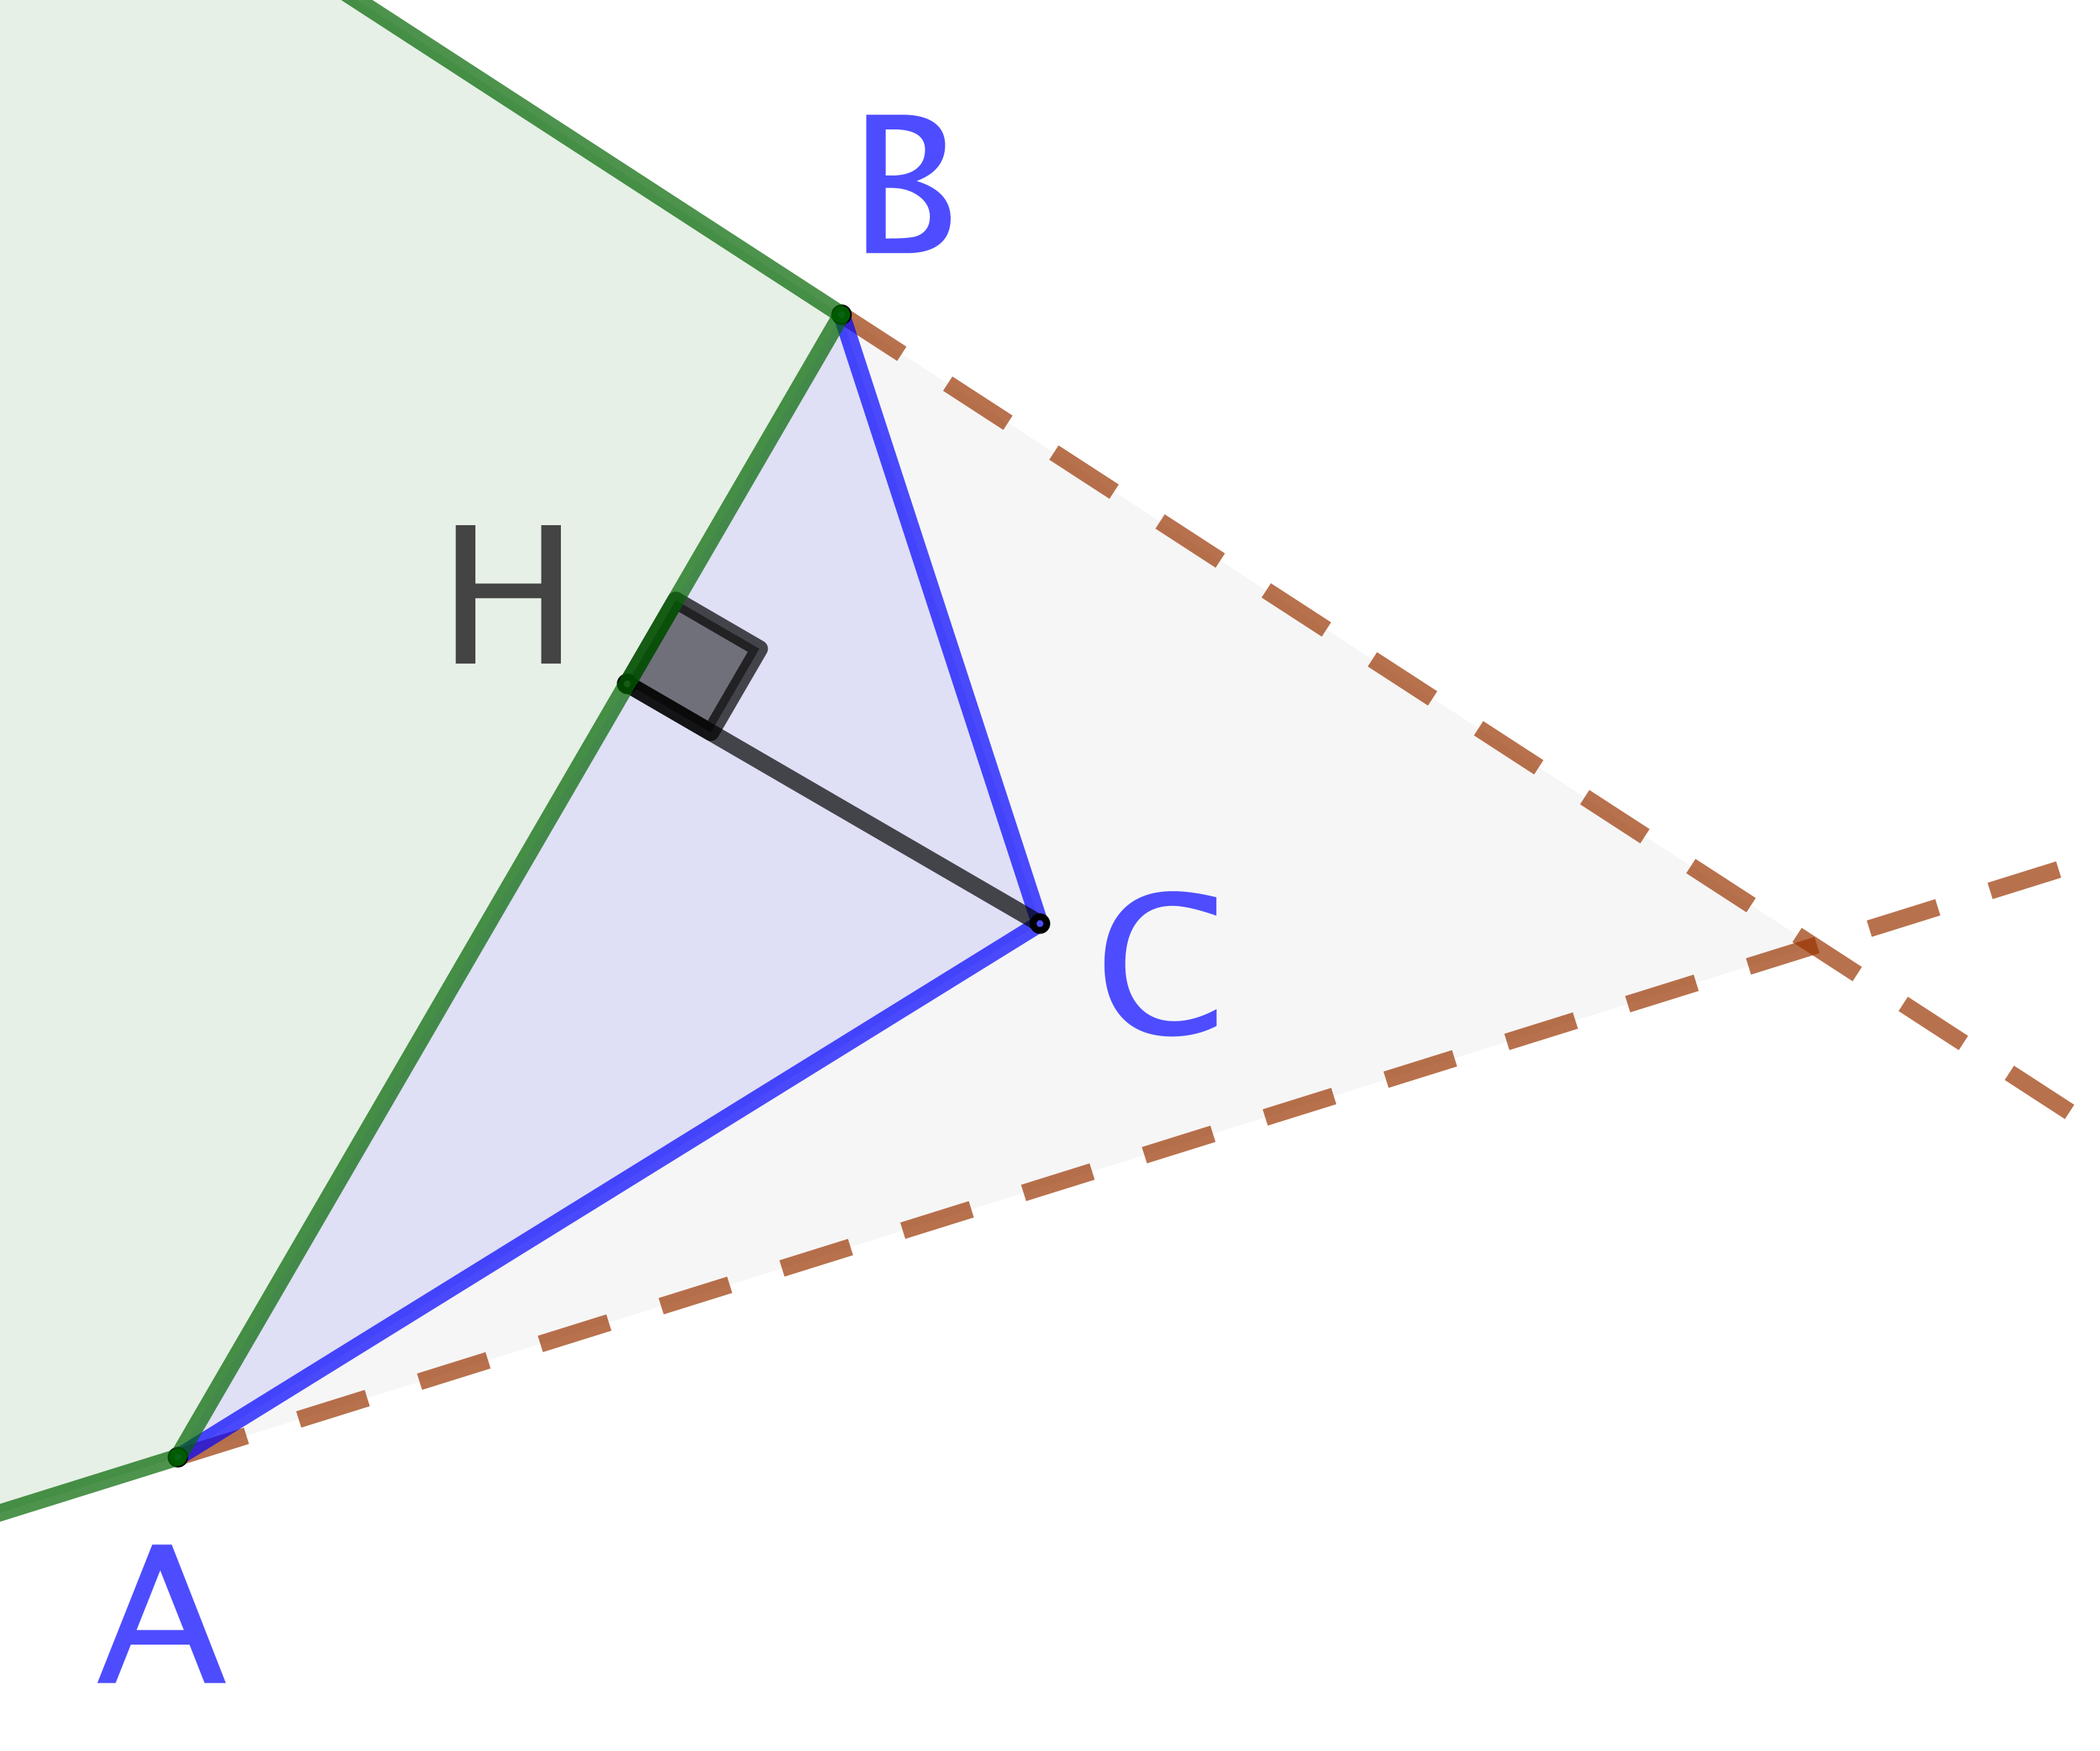
\includegraphics[scale=.4]{content/polygon/necessary-cond/add-vertex-1.png}

			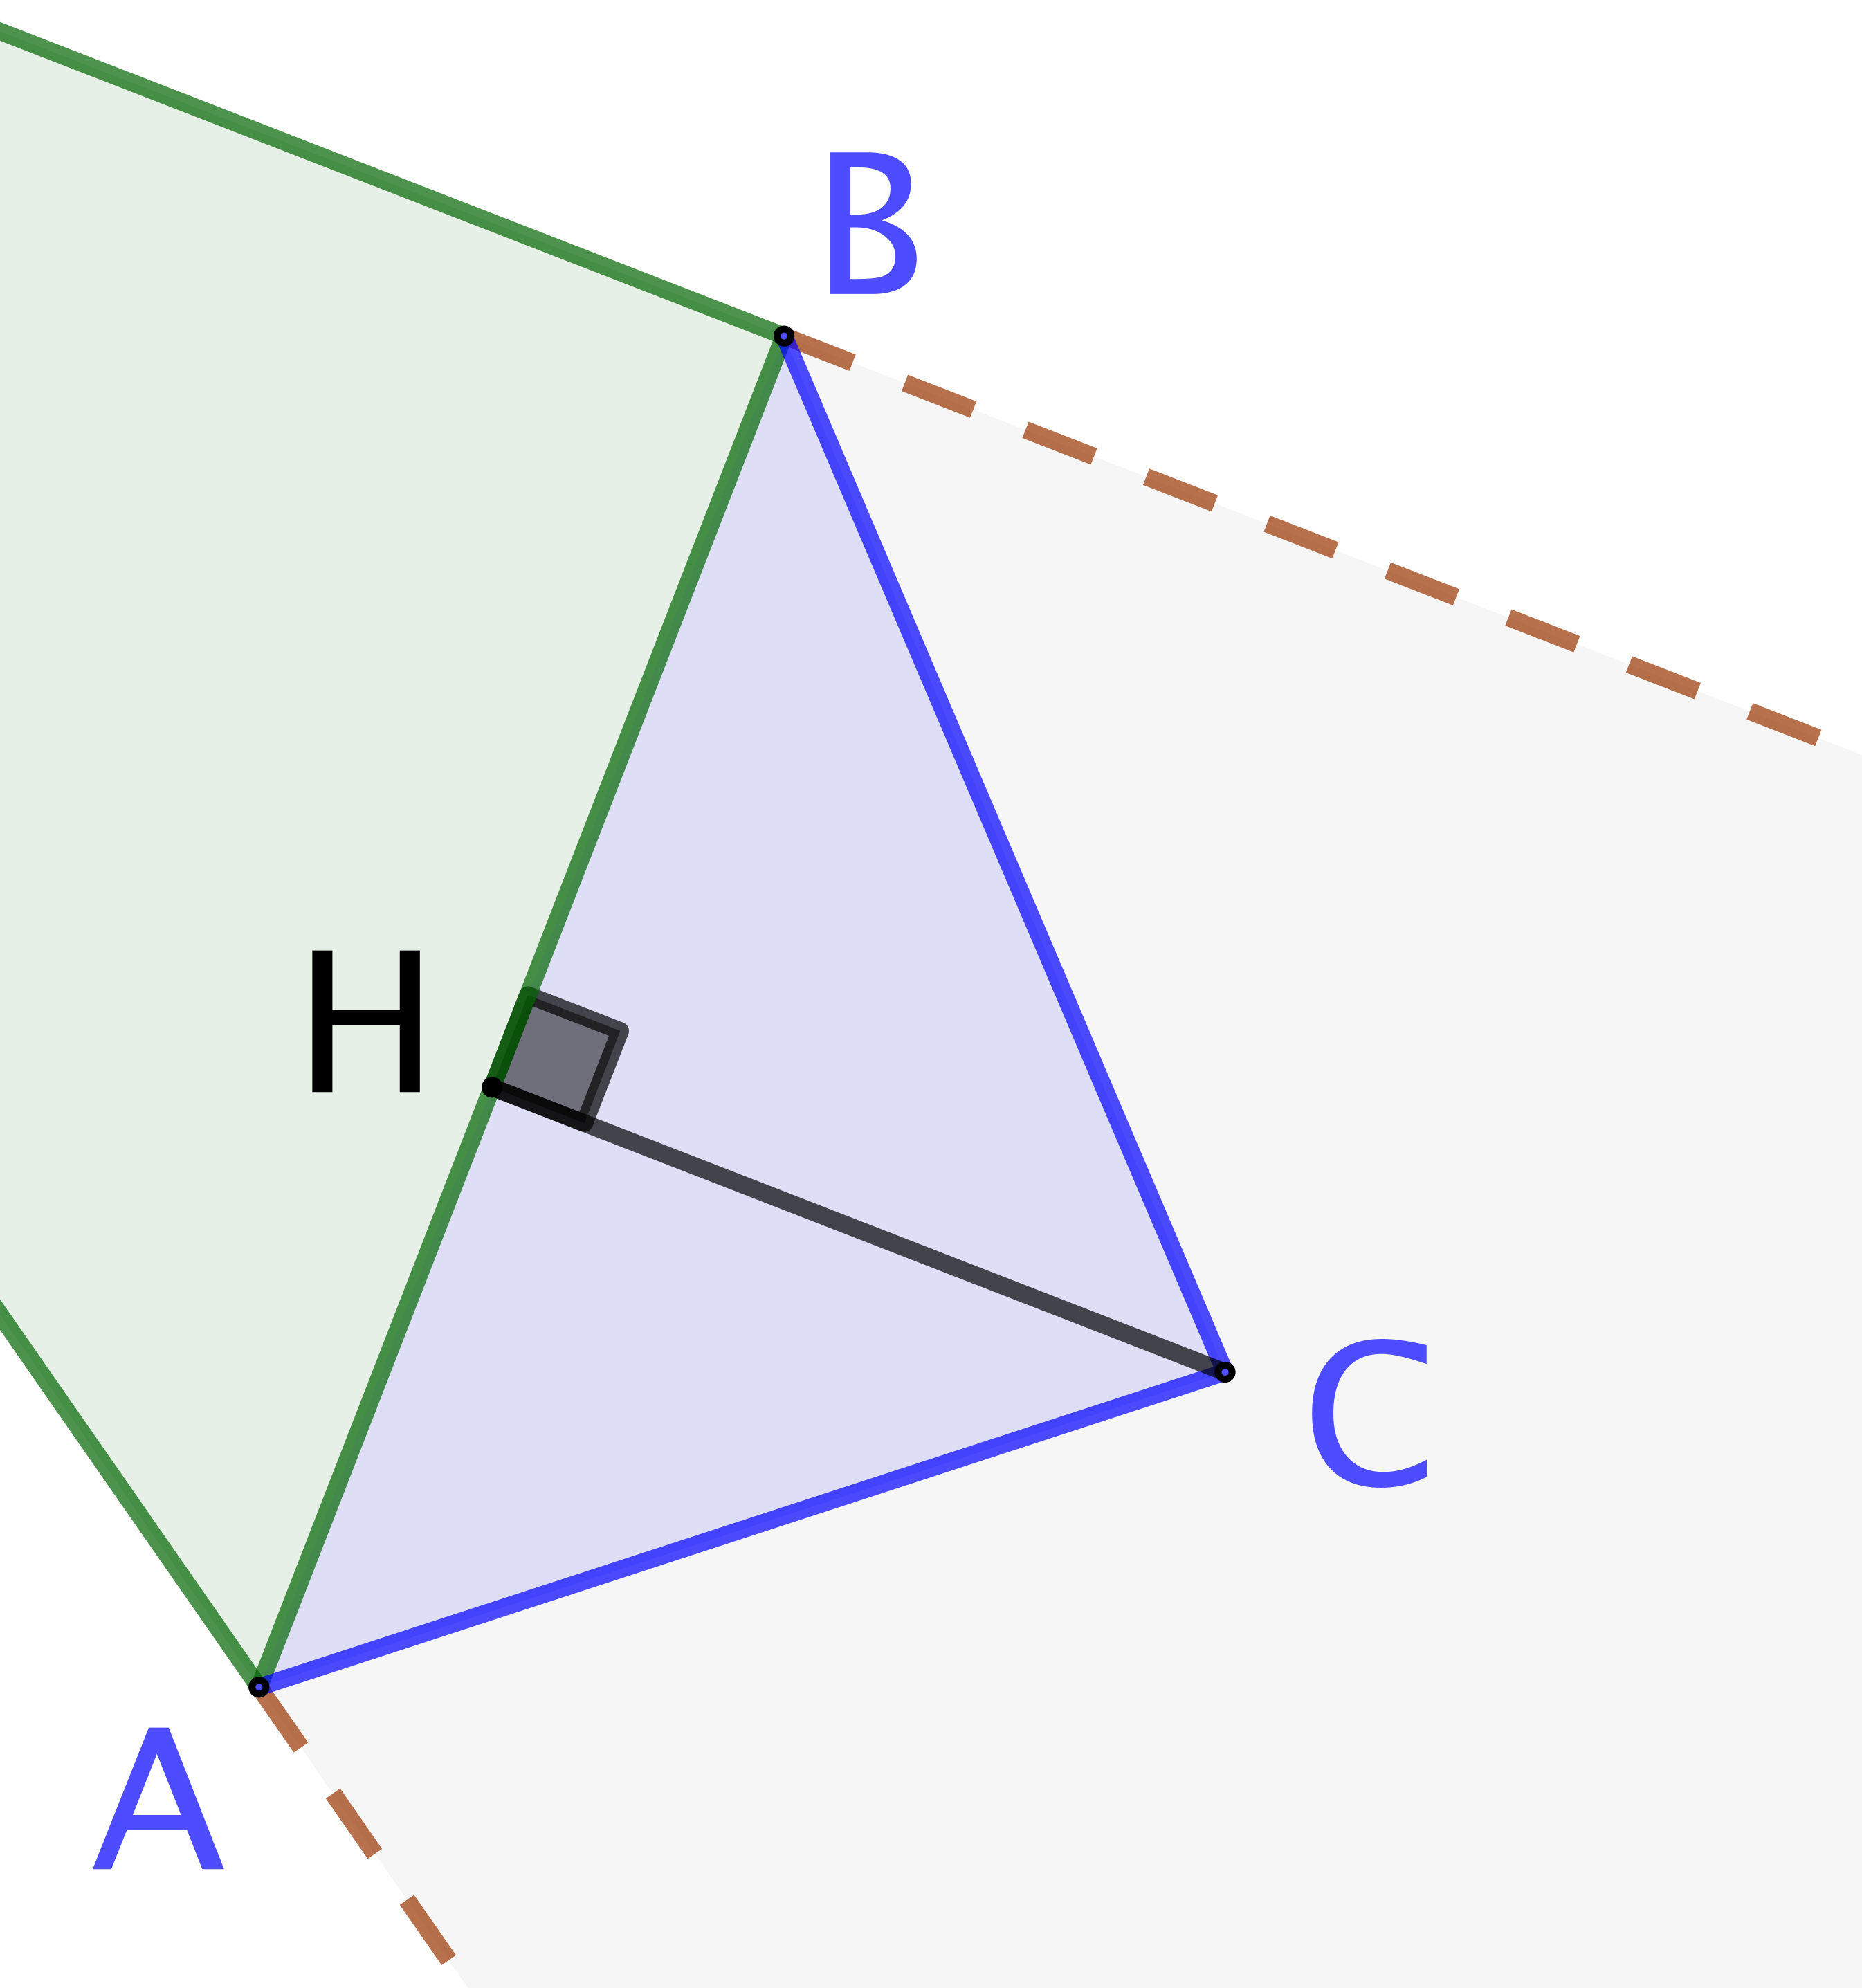
\includegraphics[scale=.4]{content/polygon/necessary-cond/add-vertex-2.png}
		\end{multicols}

		\item Clairement, le polygone $\setproba{C}^{\,\prime}$ obtenu à partir de $\setproba{C}$ en remplaçant le côté $[AB]$ par les côtés $[AC]$ et $[CB]$ est un convexe avec un sommet de plus que $\setproba{C}$.

		\item \label{add-vertex-end}
		Comme $HC$ peut être rendu aussi proche de $0$ que souhaité, il est aisé de voir que l'on peut choisir cette distance de sorte que $AC + BC < AB + \frac{\delta}{m}$.
		Dès lors, le périmètre de $\setproba{C}^{\,\prime}$ augmente de $\frac{\delta}{m}$ relativement à $\setproba{C}$.

		\item En répétant $(m-1)$ fois les étapes \ref{add-vertex-start} à \ref{add-vertex-end} avec les nouveaux \ngones\ convexes $\setproba{C}^{\,\prime}$ sans changer la valeur de $m$, nous obtenons un \ngone\ convexe $\setproba{P}^{\,\prime}$ tel que
		$\area{\setproba{P}^{\,\prime}} > \area{\setproba{P}}$
		et
		$\perim{\setproba{P}^{\,\prime}} < \perim{\setproba{C}} + \delta = \perim{\setproba{P}}$.
	\end{enumerate}
\end{proof}


\begin{remark}
	Le fait précédent permet de toujours se ramener au cas d'un \ngone\ convexe.
\end{remark}


% ----------------------- %


\begin{fact} \label{iso-poly} 
	Si un \ngone\ convexe $\setproba{P}$ n'est pas un \niso, alors on peut construire un \ngone\ convexe $\setproba{P}^{\,\prime}$ tel que 
	$\perim{\setproba{P}^{\,\prime}} = \perim{\setproba{P}}$ 
	et 
	$\area{\setproba{P}^{\,\prime}} > \area{\setproba{P}}$.
\end{fact}


\begin{proof}
	Considérons un \ngone\ convexe $\setproba{P}$ qui ne soit pas un \niso.
	Dans ce cas, $\setproba{P}$ admet un triplet de sommets consécutifs $A$, $B$ et $C$ tels que $AB \neq BC$ (sinon, on obtiendrait de proche en proche un \niso).
	La construction vue dans la preuve du fait \ref{tri-one-side-fixed} nous donne la solution: voir les deux dessins ci-après dans lesquels $(AC) \parallel (BB^{\,\prime})$. 
	Pour le 2\ieme\ cas, il n'est pas possible d'utiliser le triangle $AB^{\,\prime}C$ isocèle en $B^{\,\prime}$ car $(B^{\,\prime}C)$ porte le côté de $\setproba{P}$ de sommet $C$ juste après $[BC]$, mais ce problème se contourne en considérant un point $B^{\,\prime\prime}$ de $]BB^{\,\prime}[$.
	%	
	\begin{multicols}{2}
		\centering

		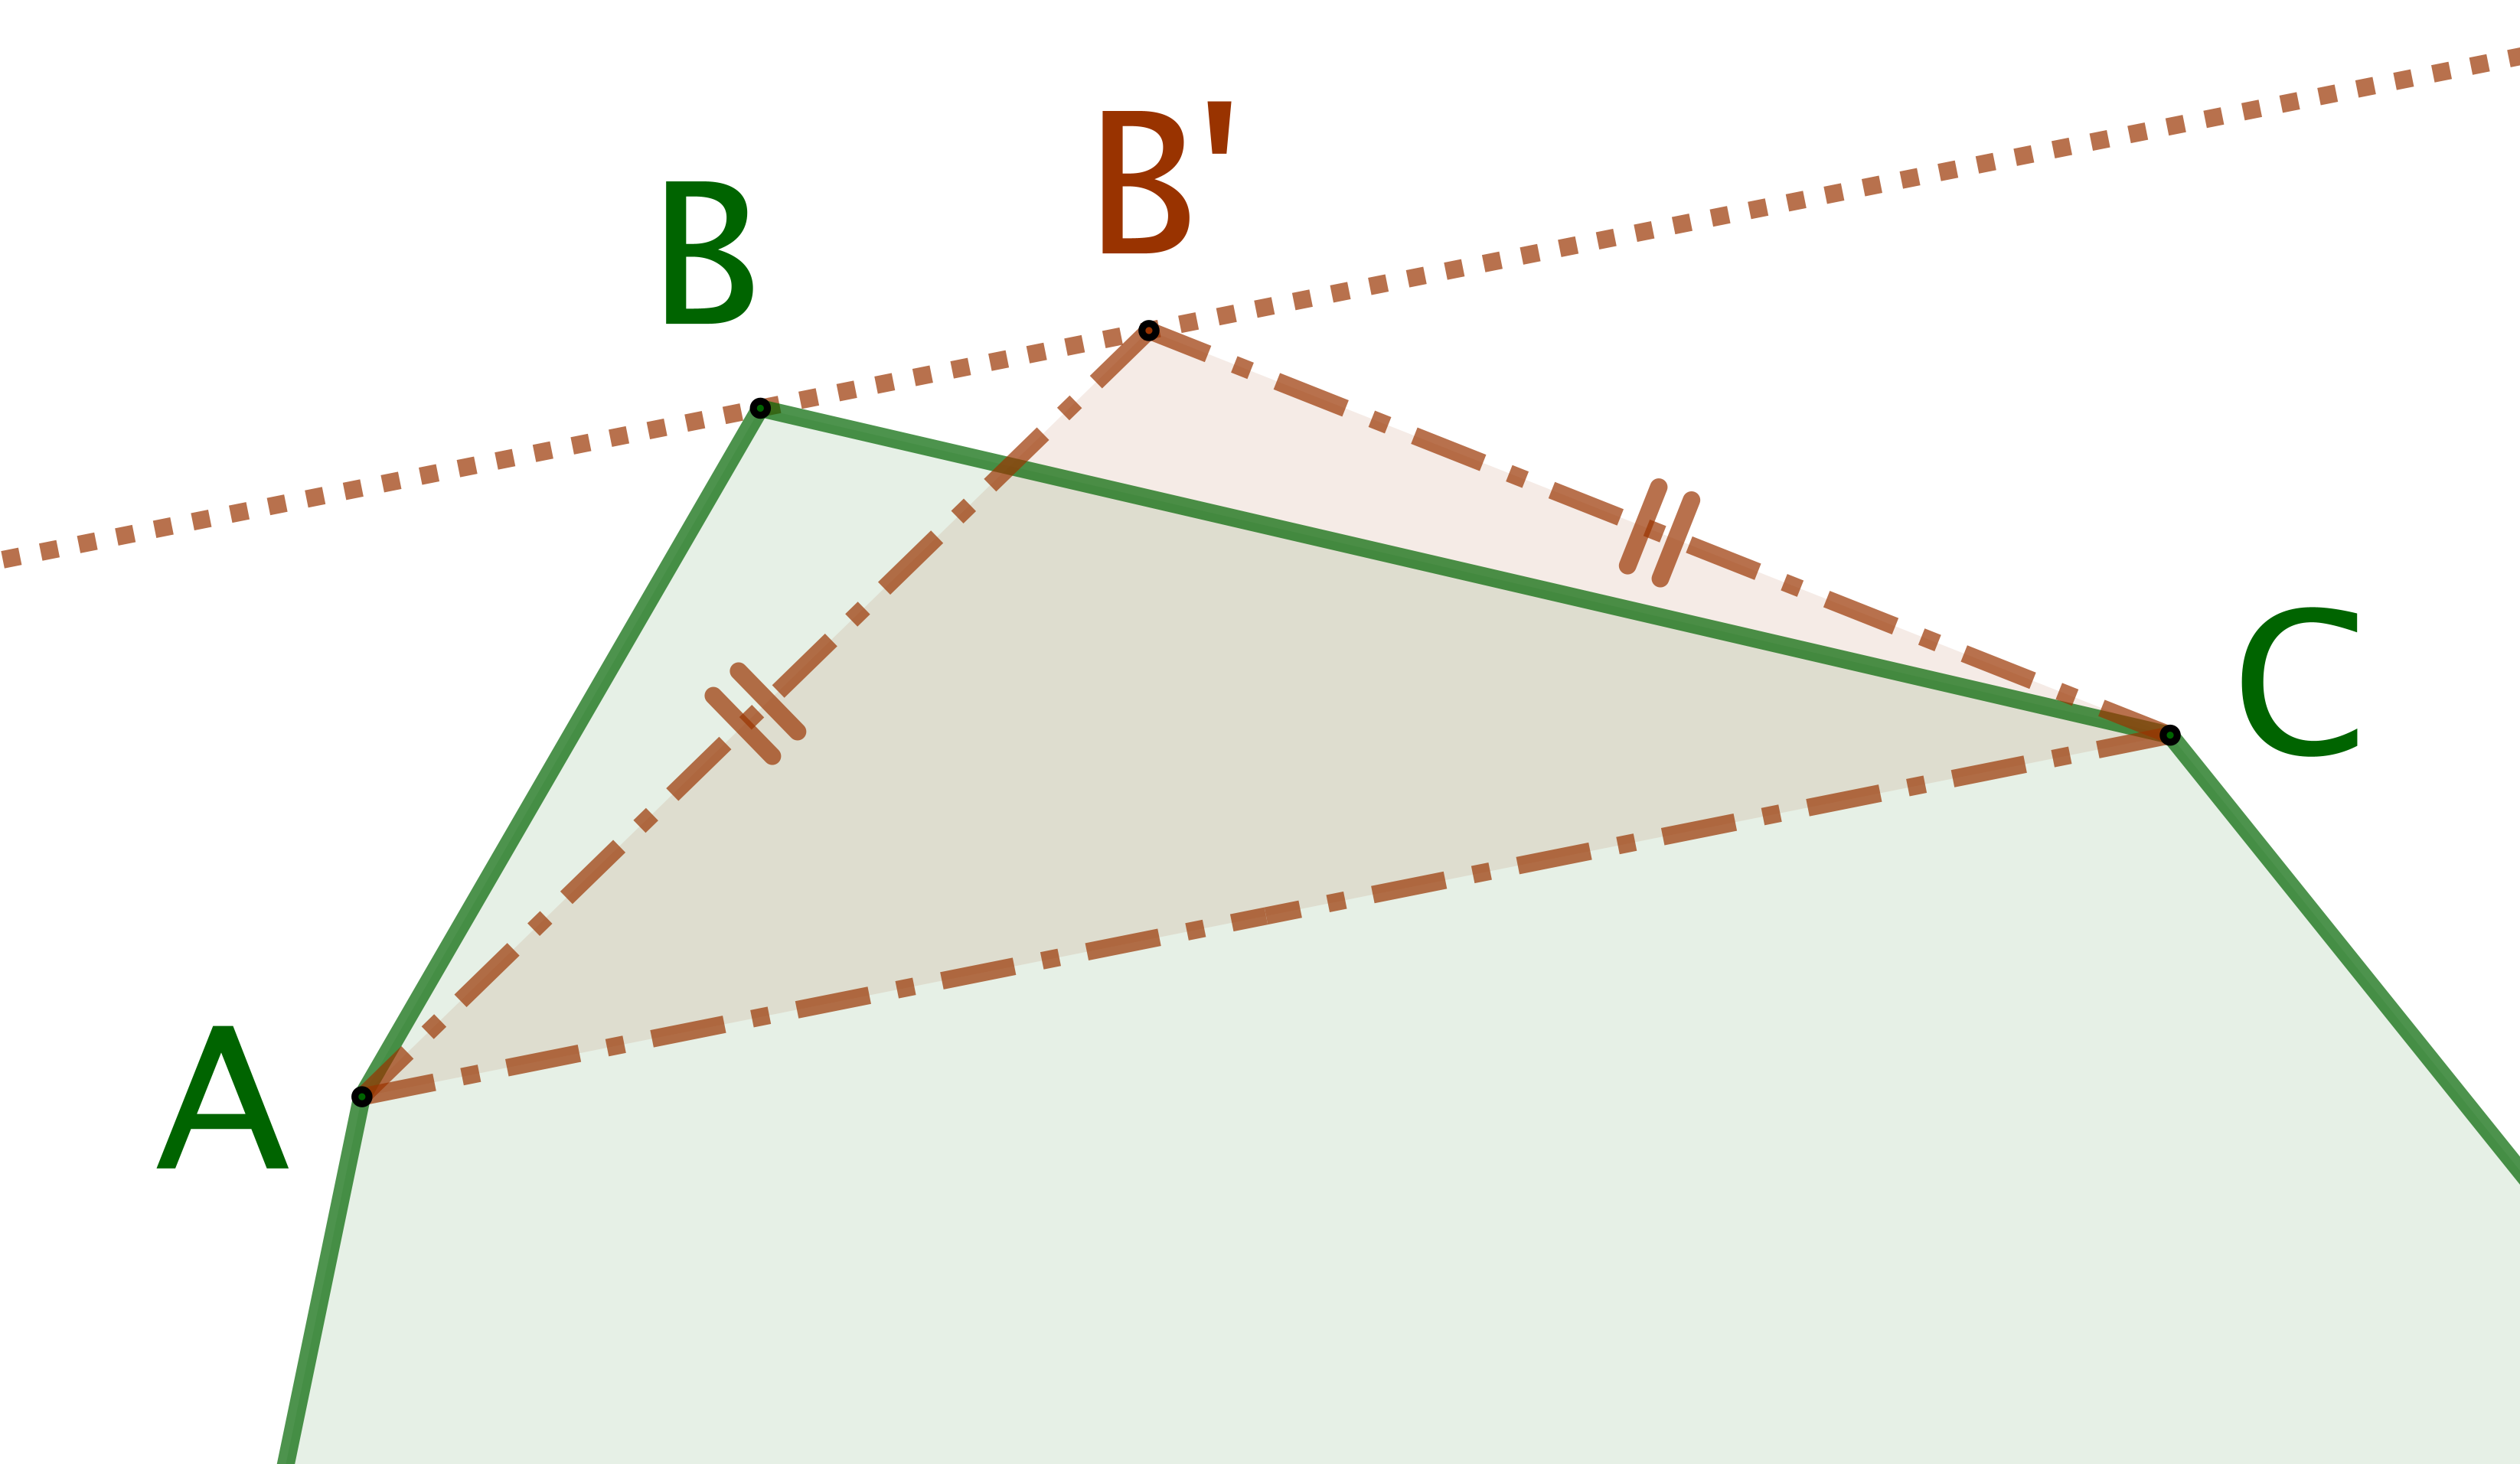
\includegraphics[scale=.4]{content/polygon/necessary-cond/not-iso-OK.png}

		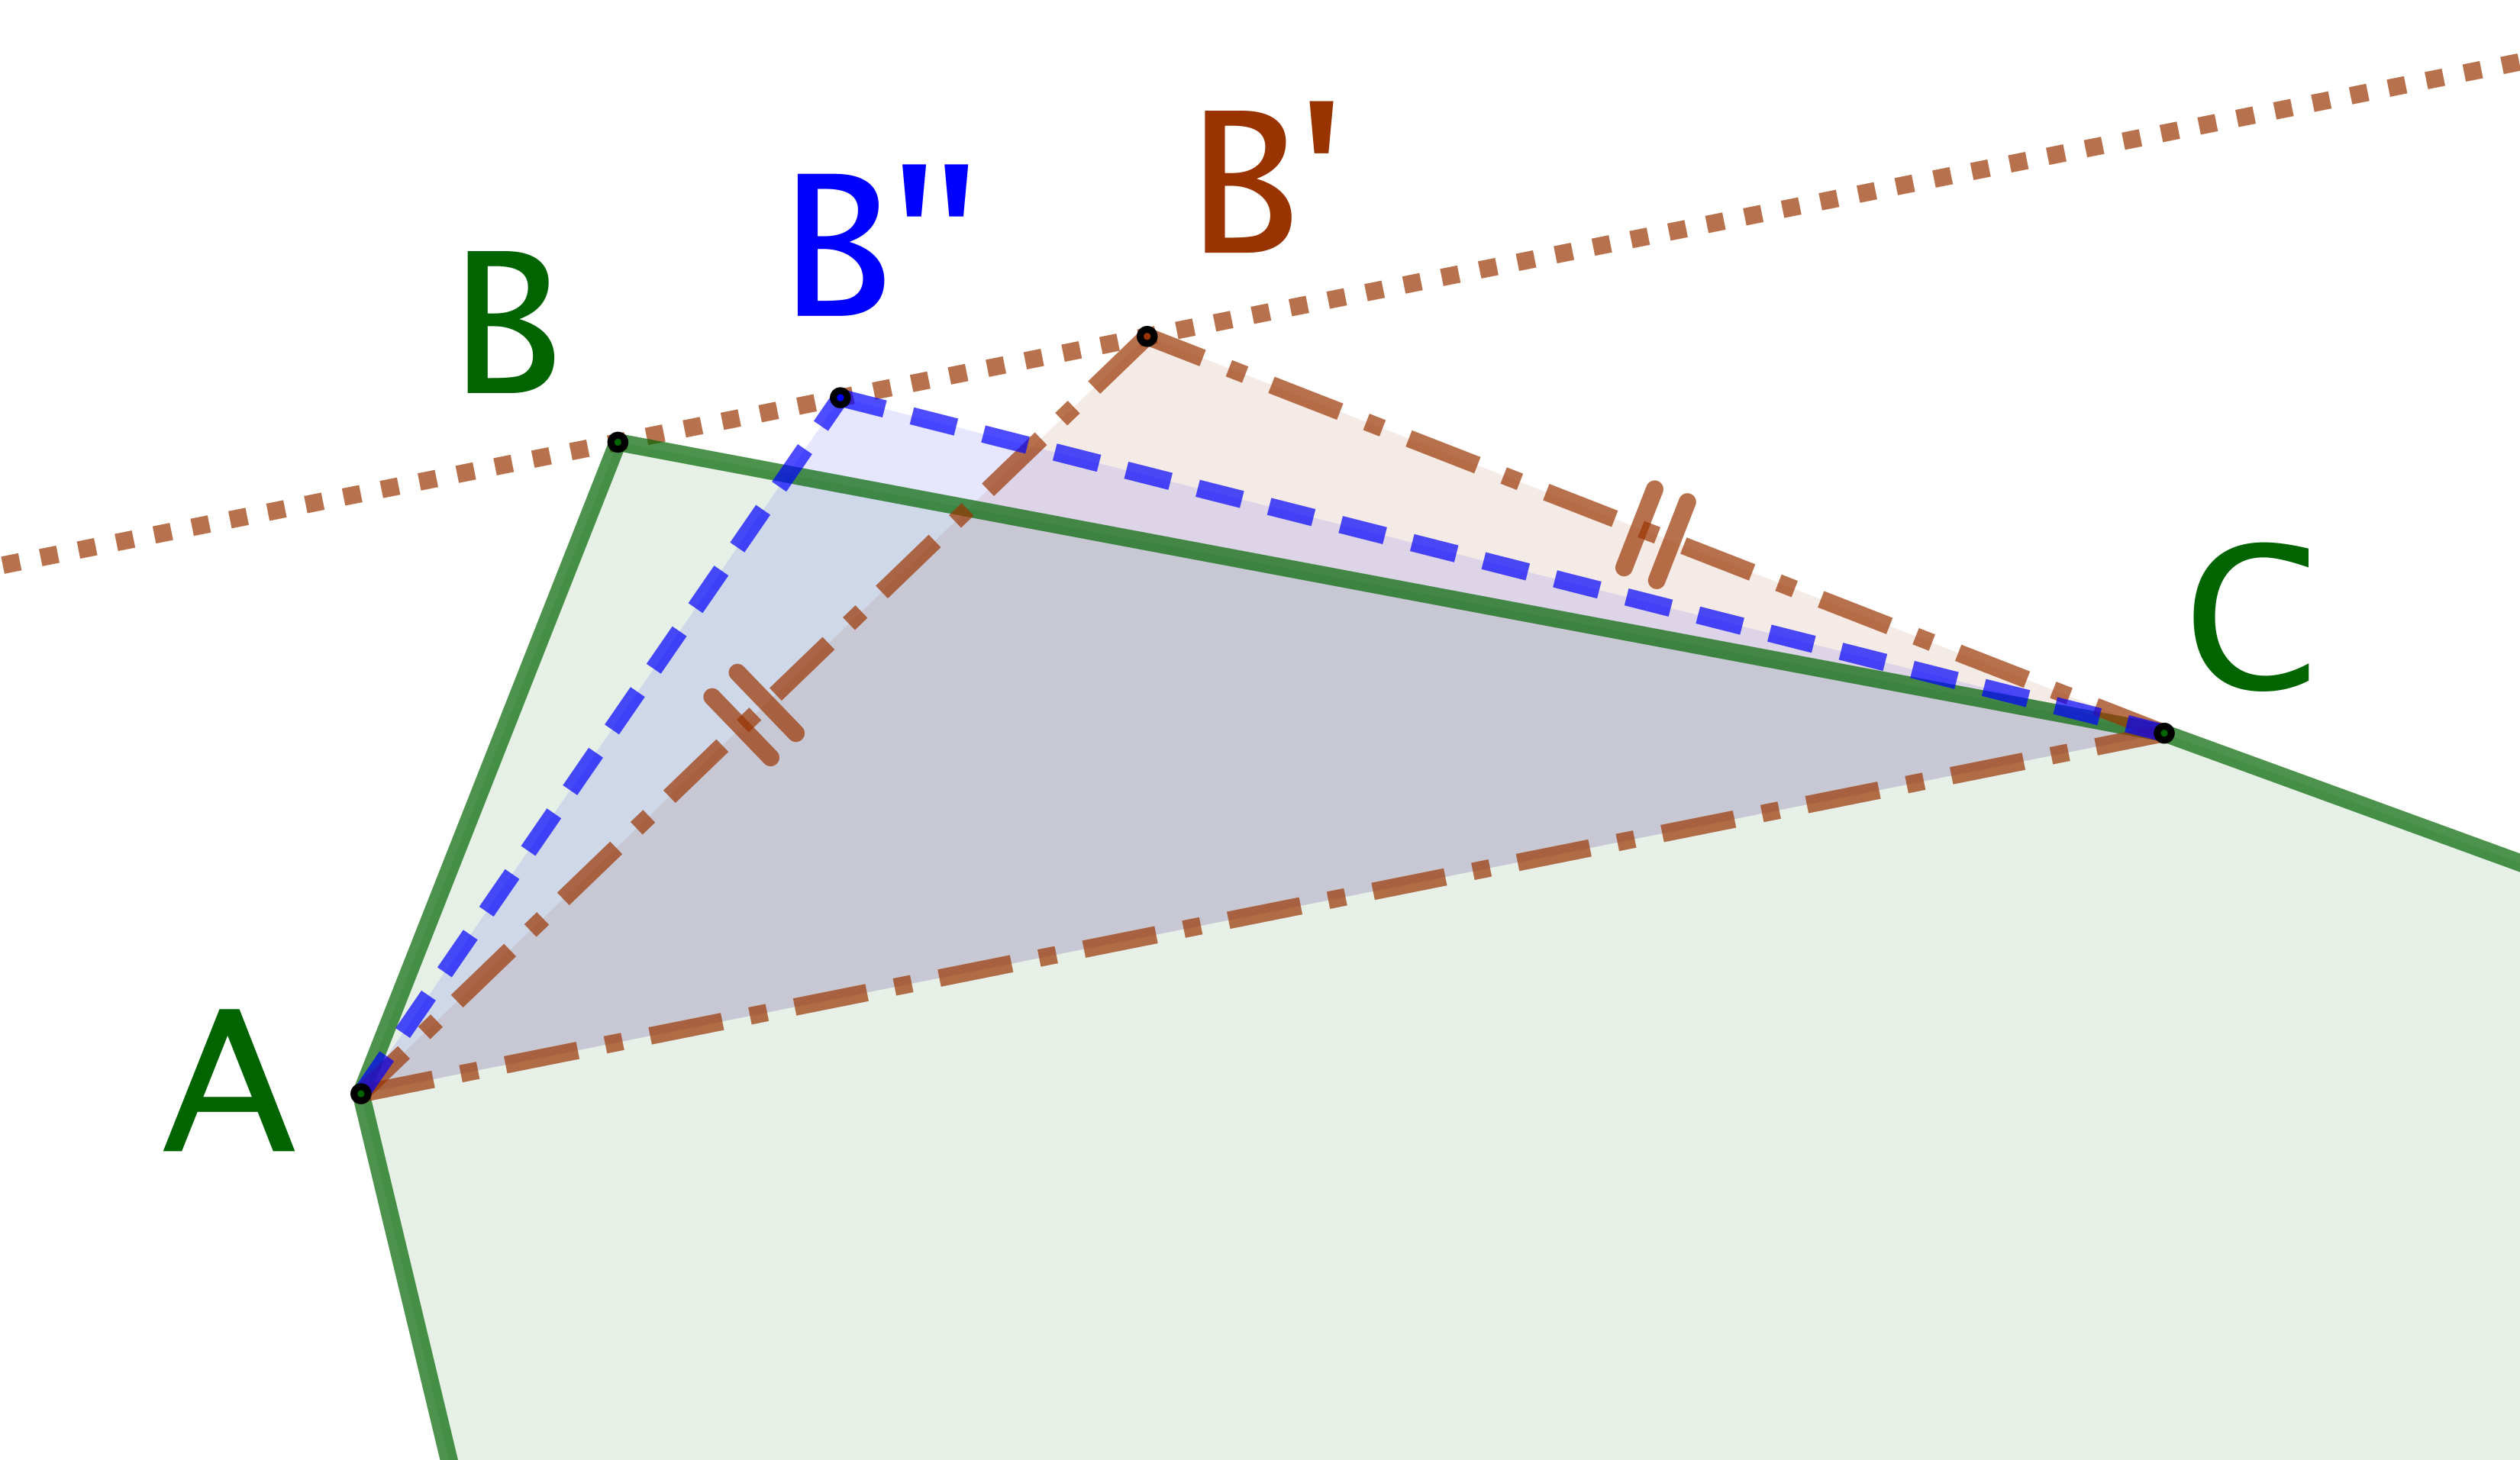
\includegraphics[scale=.4]{content/polygon/necessary-cond/not-iso-KO.png}
	\end{multicols}
	
	Dans chaque cas, nous avons construit un \ngone\ convexe $\setproba{P}^{\,\prime\prime}$ tel que 
	$\perim{\setproba{P}^{\,\prime\prime}} < \perim{\setproba{P}}$ 
	et 
	$\area{\setproba{P}^{\,\prime\prime}} = \area{\setproba{P}}$.
	Un simple agrandissement donne un \ngone\ convexe $\setproba{P}^{\,\prime}$ vérifiant
	$\perim{\setproba{P}^{\,\prime}} = \perim{\setproba{P}}$ 
	et 
	$\area{\setproba{P}^{\,\prime}} > \area{\setproba{P}}$.
\end{proof}


\begin{remark}
	Le fait précédent ne permet pas de toujours se ramener au cas d'un \niso\ convexe. Il nous dit juste que si un \ngone\ convexe maximise son aire à périmètre fixé, alors il devra être un \niso. La nuance est importante, et une similaire existe pour le fait suivant.
\end{remark}


% ----------------------- %


\begin{fact} \label{almost-reg-poly}
	Si un \niso\ convexe $\setproba{P}$ possède deux angles de mesures différentes,
	alors il existe un \ngone\ convexe $\setproba{P}^{\,\prime}$ tel que
	$\perim{\setproba{P}^{\,\prime}} = \perim{\setproba{P}}$ 
	et 
	$\area{\setproba{P}^{\,\prime}} > \area{\setproba{P}}$.
\end{fact}


\begin{proof}
	Par hypothèse, nous avons deux paires de côtés 
	$\big( [AB] , [BC] \big)$ et 
	$\big( [EF] , [FG] \big)$ tels que 
	$\anglein{ABC} > \anglein{EFG}$.
	Par convexité de $\setproba{P}$, nous avons juste à augmenter la somme des aires des triangles $ABC$ et $EFG$.
	Nous allons le faire en modifiant les angles $\anglein{ABC}$ et $\anglein{EFG}$ tout en gardant $AB = BC = EF = FG$.
	%	
	\begin{multicols}{2}
		\centering

		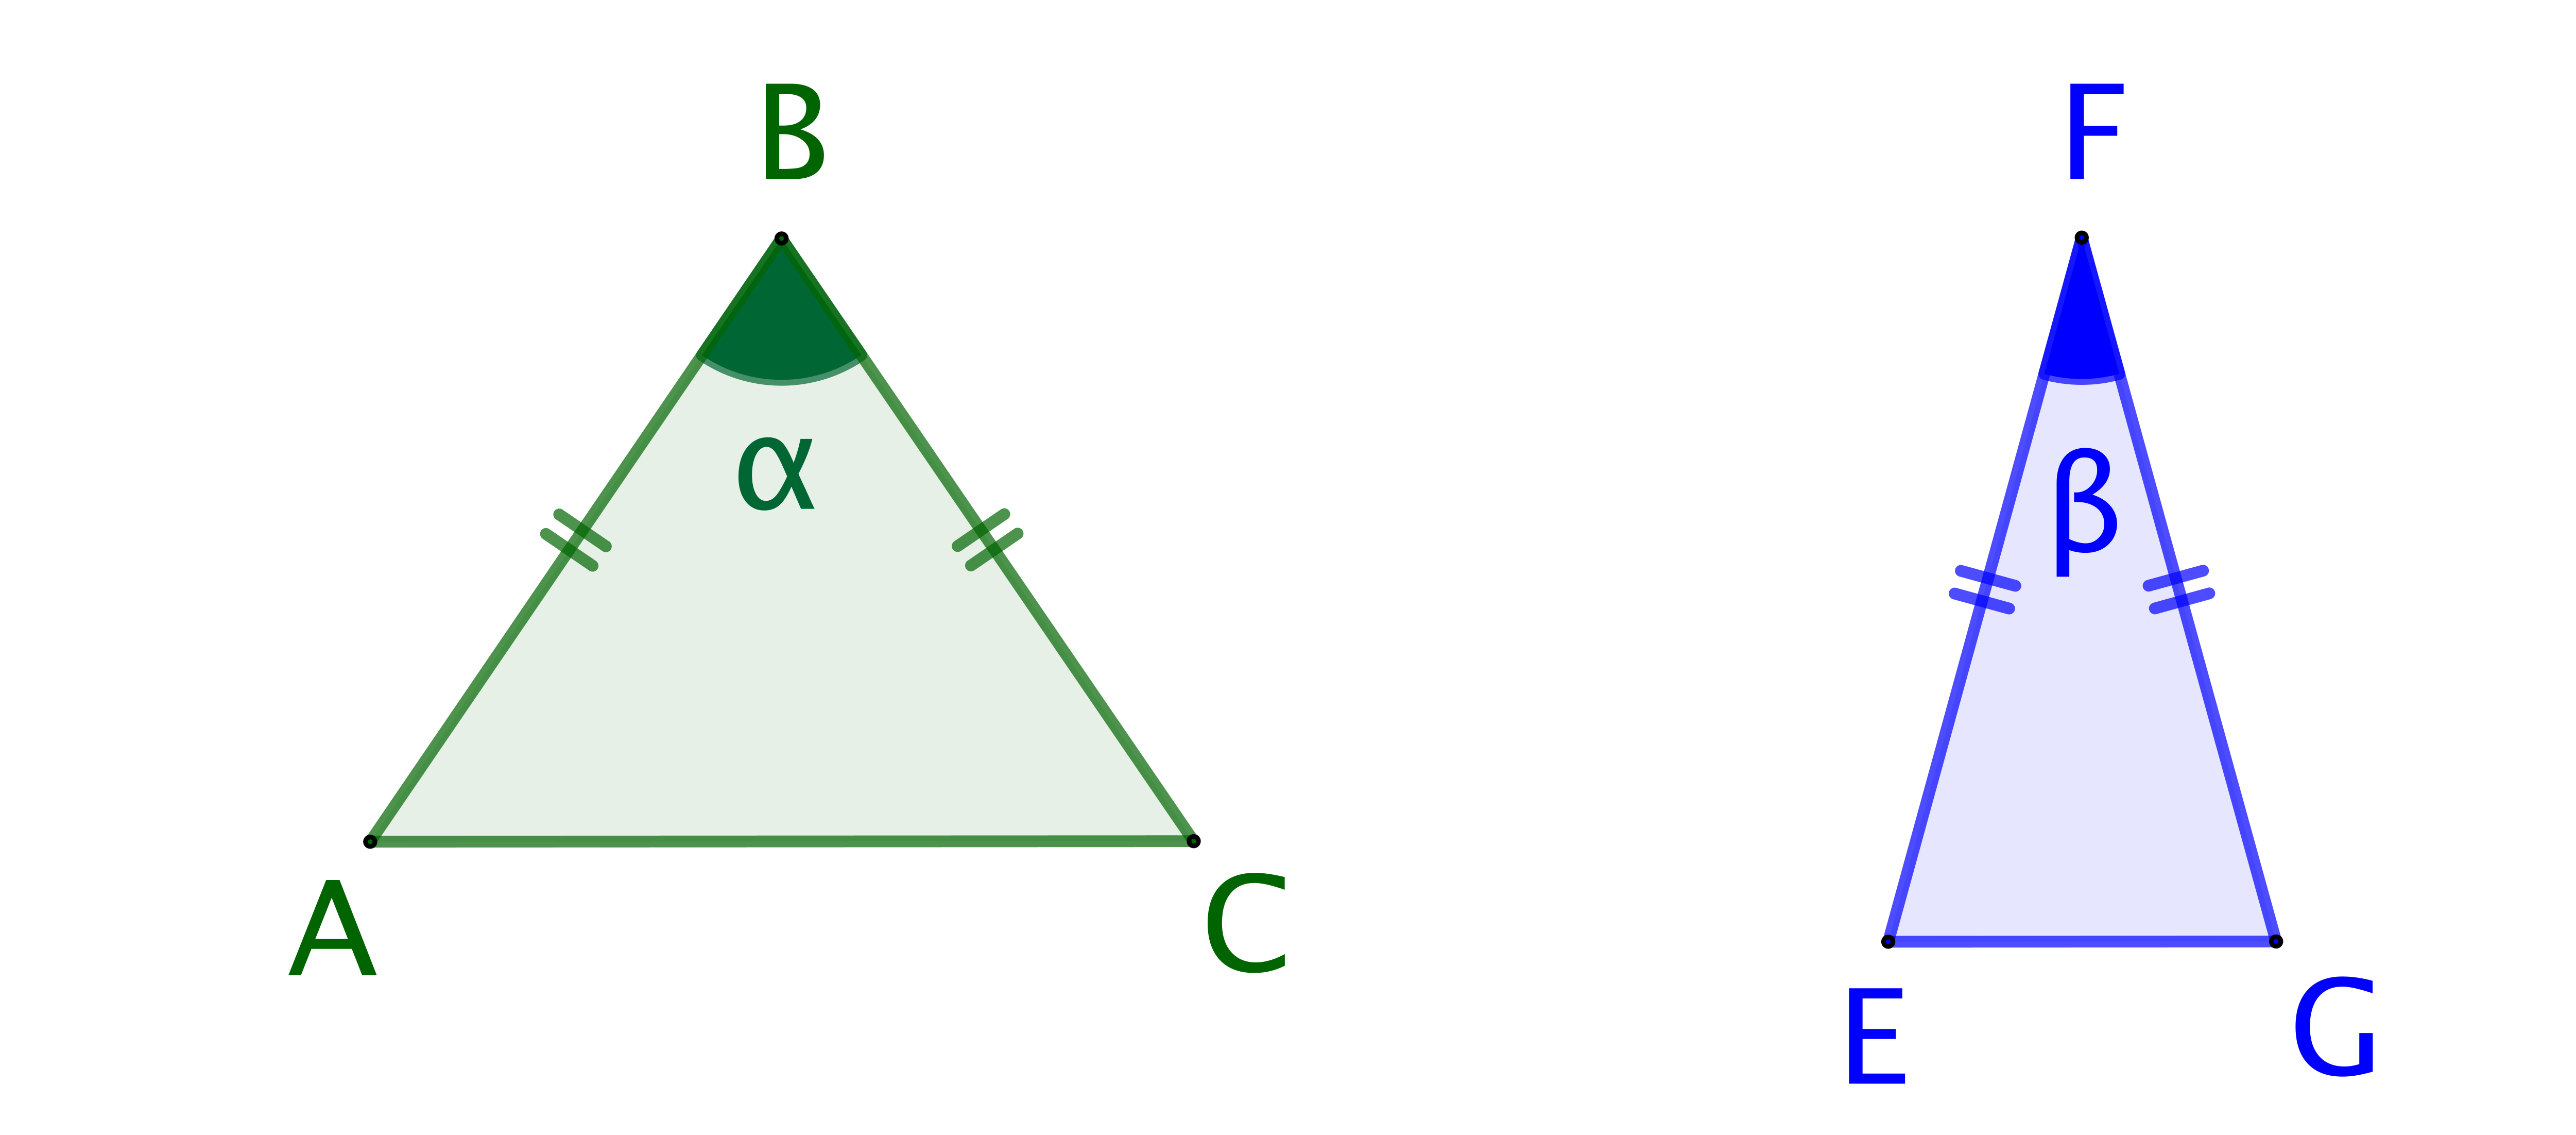
\includegraphics[scale=.4]{content/polygon/necessary-cond/2-eq-angles-1.png}

		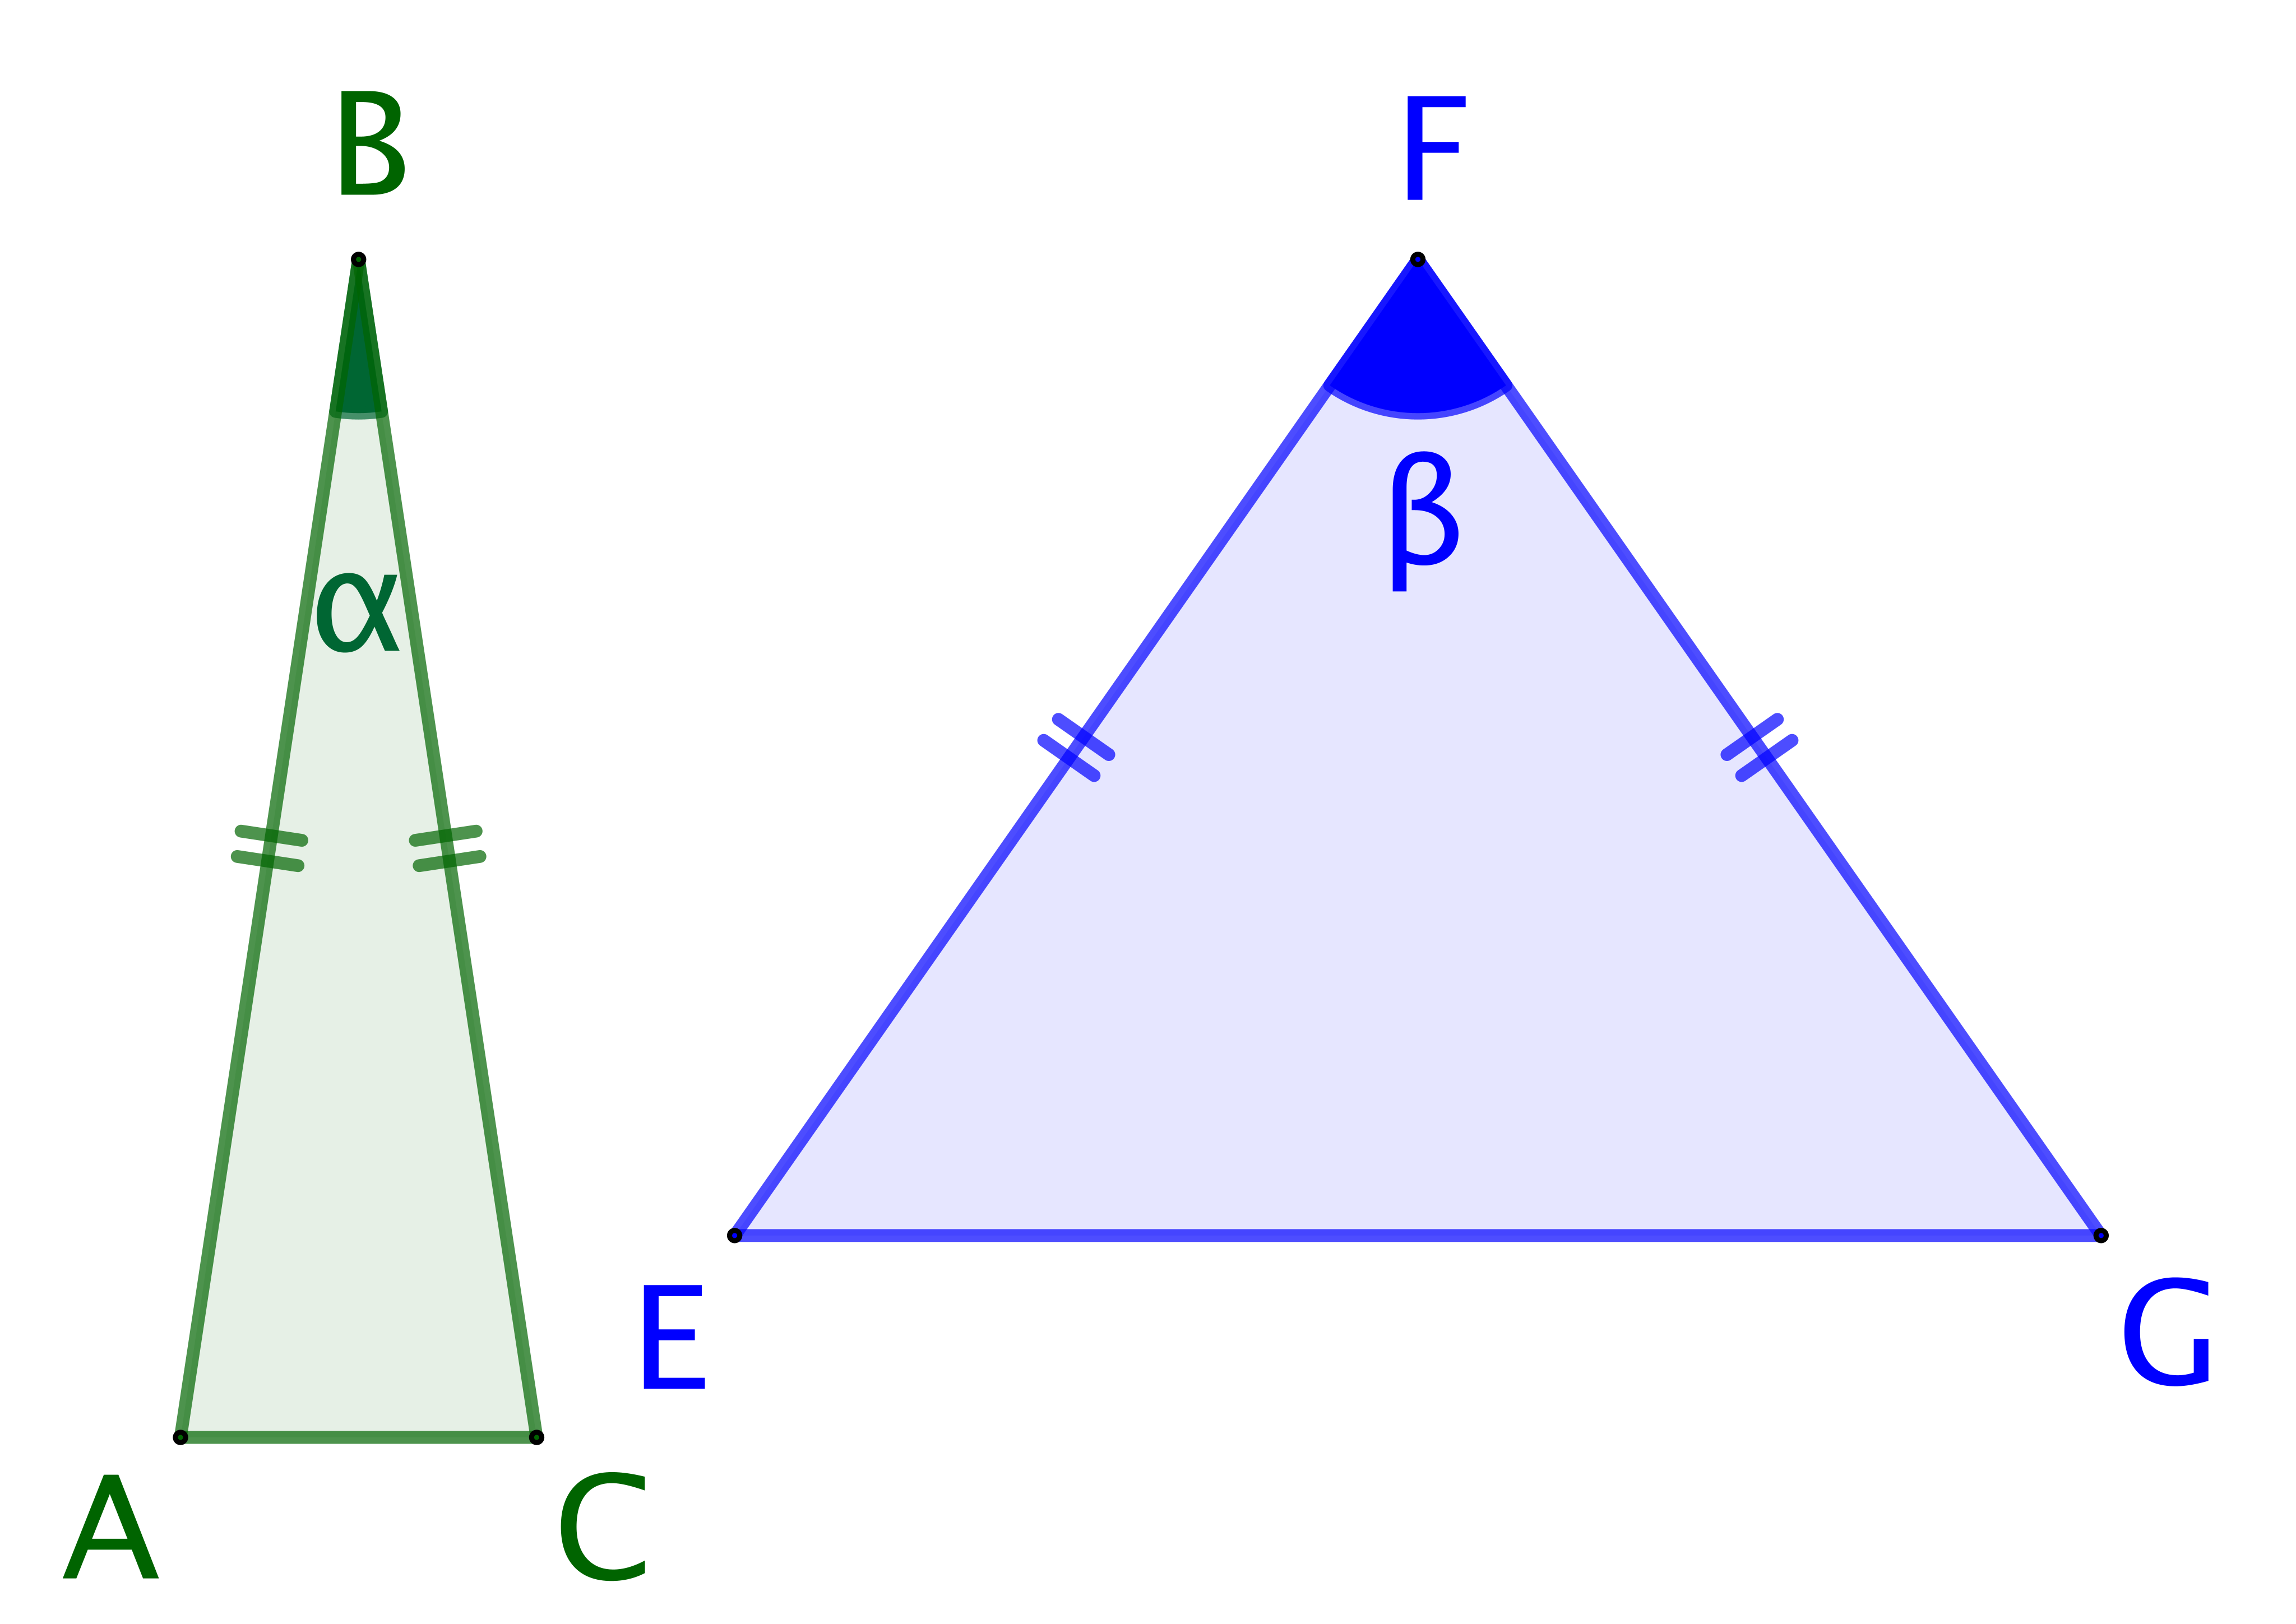
\includegraphics[scale=.4]{content/polygon/necessary-cond/2-eq-angles-2.png}
	\end{multicols}

	Les deux exemples ci-dessus nous permettent de noter que si $\alpha = \anglein{ABC}$ diminue, et $\beta = \anglein{EFG}$ augmente, alors la somme des aires se rapprochent de $0$.
	Par raison de symétrie, si on fixe $\anglein{ABC} + \anglein{EFG}$, on devine que la somme des aires est maximisée quand $\anglein{ABC} = \anglein{EFG}$.
	Nous allons établir ceci de façon élémentaire en commençant par les calculs suivants où 
	$\ell = AB$, 
	$\mu = \frac{\alpha + \beta}{2}$ et 
	$\delta = \mu - \beta > 0$ (rappelons que nous avons supposé $\alpha > \beta$). 
	
	\medskip	
	\begin{stepcalc}[style=ar*]
		\area{ABC} + \area{EFG}
	\explnext*{Formule dite des sinus.}{}
		\dfrac12 BA \cdot BC \cdot \sin \big( \anglein{ABC} \big)
		+
		\dfrac12 FE \cdot FG \cdot \sin \big( \anglein{EFG} \big)
	\explnext{}
		\dfrac12 \ell^2 ( \sin \alpha + \sin \beta )
	\explnext*{Formules de Simpson.}{}
		\dfrac12 \ell^2 \sin \big( \dfrac{\alpha + \beta}{2} \big) \cos \big( \dfrac{\alpha - \beta}{2} \big)
	\explnext{}
		\dfrac12 \ell^2 \sin \mu \cos \delta
	\end{stepcalc}
	
	
	\medskip
	
	Comme $(\delta ; \mu) \in \intervalO{0}{\pi}^2$,
	nous avons $\sin \mu \cos \delta > \sin \mu$.
	Remplaçons alors $\alpha$ et $\beta$ respectivement par $\alpha^{\,\prime}$ et $\beta^{\,\prime}$ de telle sorte que $\alpha^{\,\prime} = \beta^{\,\prime} = \frac{\alpha + \beta}{2} = \mu$.
	Notons que 
	$0 < \beta < \mu < \alpha < \pi$ 
	(diminution de $\alpha$ et augmentation de $\beta$).
	Deux situations se présentent à nous.
	%
	\begin{itemize}
		\item Le \ngone\ obtenu ne perd aucun côté.
		Comme la convexité est gardée, c'est gagné.

		\item Le \ngone\ obtenu perd au moins un côté. La solution consiste à choisir
		$\alpha^{\,\prime\prime} = \mu + \frac{\delta}{2}$ et $\beta^{\,\prime\prime} = \mu - \frac{\delta}{2}$
		au lieu de
		$\alpha^{\,\prime} = \beta^{\,\prime} = \mu$, puisque nous avons
		$\cos \delta < \cos \big( \frac{\delta}{2} \big)$ et
		$0 < \beta < \beta^{\,\prime\prime} < \mu < \alpha^{\,\prime\prime} < \alpha < \pi$.
	\end{itemize}
\end{proof}


% ----------------------- %


\begin{remark} 
	La méthode des extrema liés, rappelée dans la remarque \ref{constrained-extrema}, donne une autre justification de la conjecture faite dans la démonstration précédente. Voici comment faire.
	%
	\begin{itemize}
		\item Pour $(\alpha ; \beta) \in \intervalO{0}{\pi}^2$, on veut maximiser $f(\alpha ; \beta) =  \sin \alpha + \sin \beta$ sous la contrainte $g(\alpha ; \beta) = 0$ où $g(\alpha ; \beta) = \alpha + \beta - 2 \mu$.
		
		\item
    	$\exists \lambda \in \RR$ tel que
    	$\pder[i]{f}{\alpha}{1} = \lambda \pder[i]{g}{\alpha}{1}$ et
    	$\pder[i]{f}{\beta}{1} = \lambda \pder[i]{g}{\beta}{1}$
		d'après la méthode des extrema liés.

		\item Donc
		$\cos \alpha = \cos \beta$,
		et par conséquent
		$\alpha = \beta = \mu$.
	\end{itemize}
\end{remark}


% ----------------------- %


\begin{fact} \label{nece-cond}
	Si un \ngone\ $\setproba{P}$ n'est pas régulier,
	alors il existe un \ngone\ convexe $\setproba{P}^{\,\prime}$ tel que
	$\perim{\setproba{P}^{\,\prime}} = \perim{\setproba{P}}$ 
	et 
	$\area{\setproba{P}^{\,\prime}} > \area{\setproba{P}}$.
\end{fact}


\begin{proof}
	Le fait \ref{conv-poly} permet de considérer le problème de maximisation d'aire à périmètre fixé juste pour des \ngones\ convexes.
	Selon les faits \ref{iso-poly} et \ref{almost-reg-poly}, si parmi les \ngones\ convexes de périmètre fixé, il en existe un d'aire maximale, alors ce ne peut être que le \ngone\ régulier.
\end{proof}

%
%
%\subsection{Condition suffisante}
Selon le fait \ref{nece-cond}, si parmi les \ngones\ de périmètre fixé, il en existe un qui maximise l'aire, alors ce ne peut être que le \ngone\ régulier. Nous allons établir que cette condition nécessaire est suffisante. Pour cela, nous avons juste besoin de savoir qu'il existe au moins un \ngone\ d'aire maximale.
Comme dans la remarque \ref{tri-topo-comp}, nous allons convier le couple continuité/compacité, mais ici les choses se compliquent, car nous allons devoir accepter de travailler avec des polygones croisés, et par conséquent il nous faut un moyen de mesurer la surface de tels polygones (le vrai point délicat est ici). 
Plaçons-nous d'un point de vue informatique: comme on sait calculer l'aire d'un triangle via le calcul d'un déterminant,%
\footnote{
	Il est connu que $\area{ABC} = \dfrac12 \abs{\det \big( \vect{AB} , \vect{AC} \big)}$.
}
il est naturel de chercher à calculer l'aire d'un \ngone\ en utilisant des triangles. Voici une méthode possible qui a priori pourrait dépendre du point $\Omega$ employé (le fait \ref{garea-pt-ct}, donné plus bas, justifiera le bien fondé de cette méthode).

\begin{multicols}{2}
	\small\itshape
    \begin{center}
        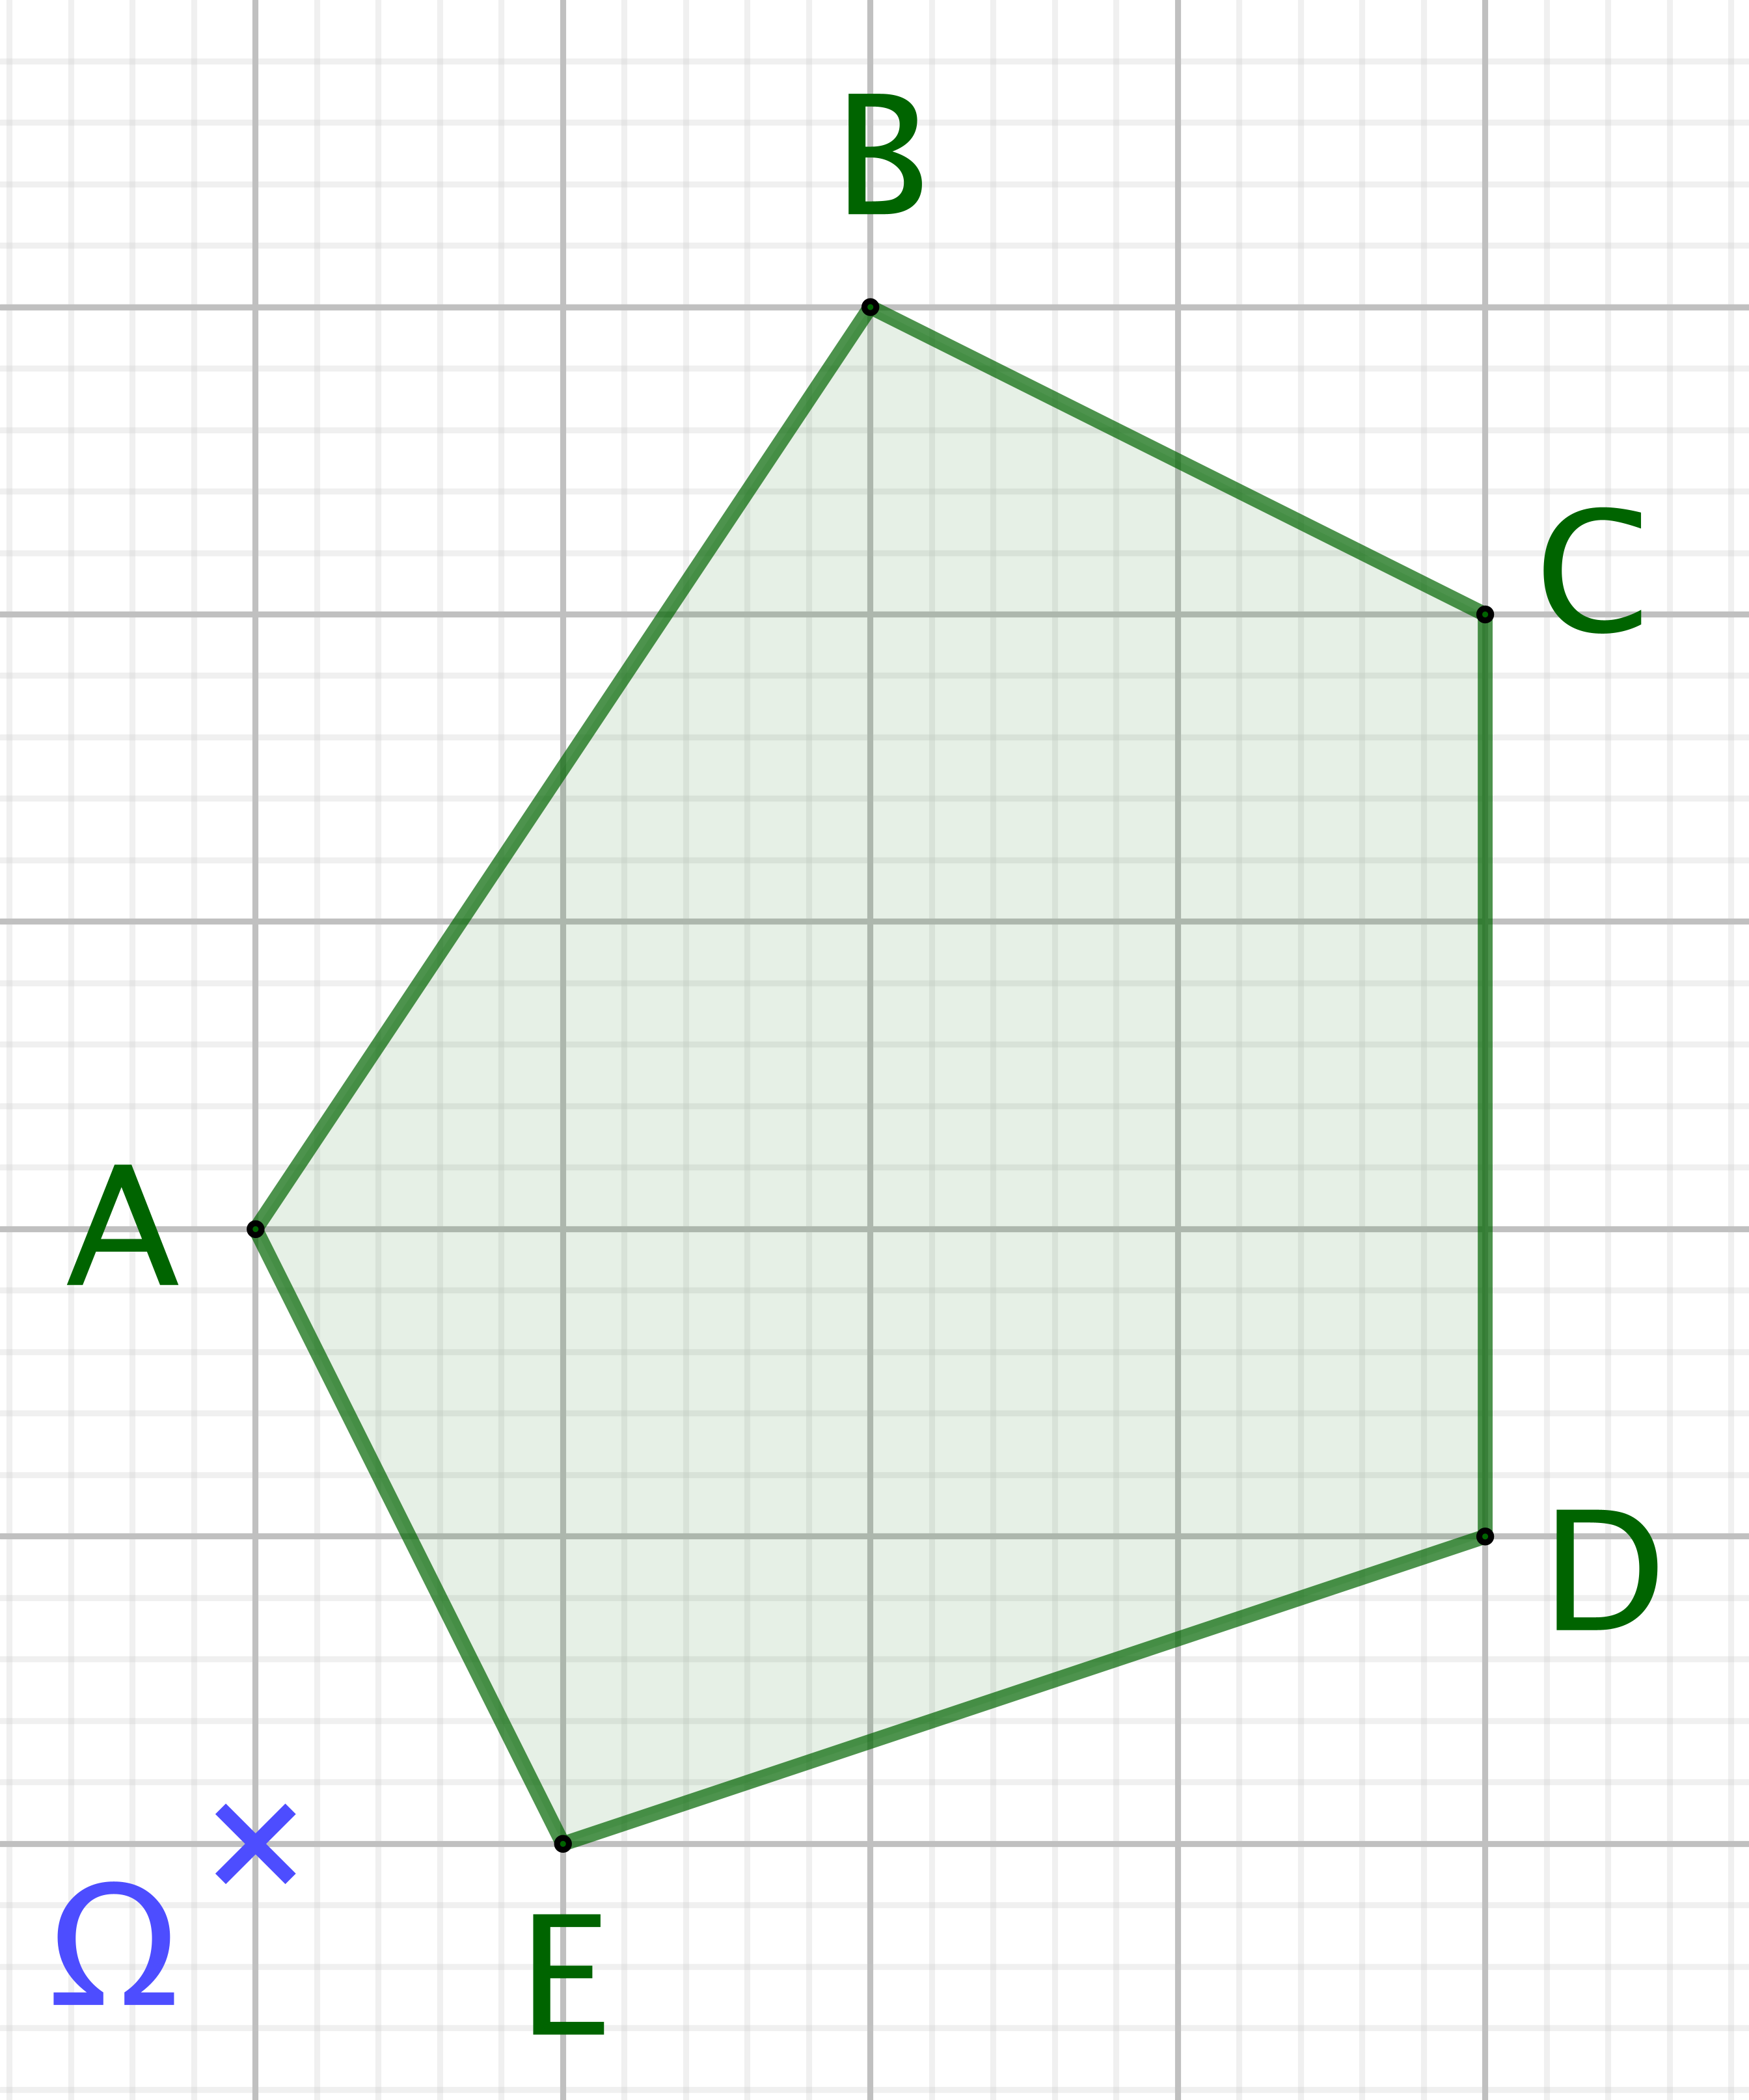
\includegraphics[scale=.4]{content/polygon/sufficient-cond/convex-1.png}
        
       	\smallskip
	
		$\num{14.5} = 4 \cdot 6 - \dfrac{2 \cdot 4 + 2 \cdot 1 + 3 \cdot 2 + 1 \cdot 3}{2}$
    \end{center}

	\columnbreak
	
    \begin{center}
        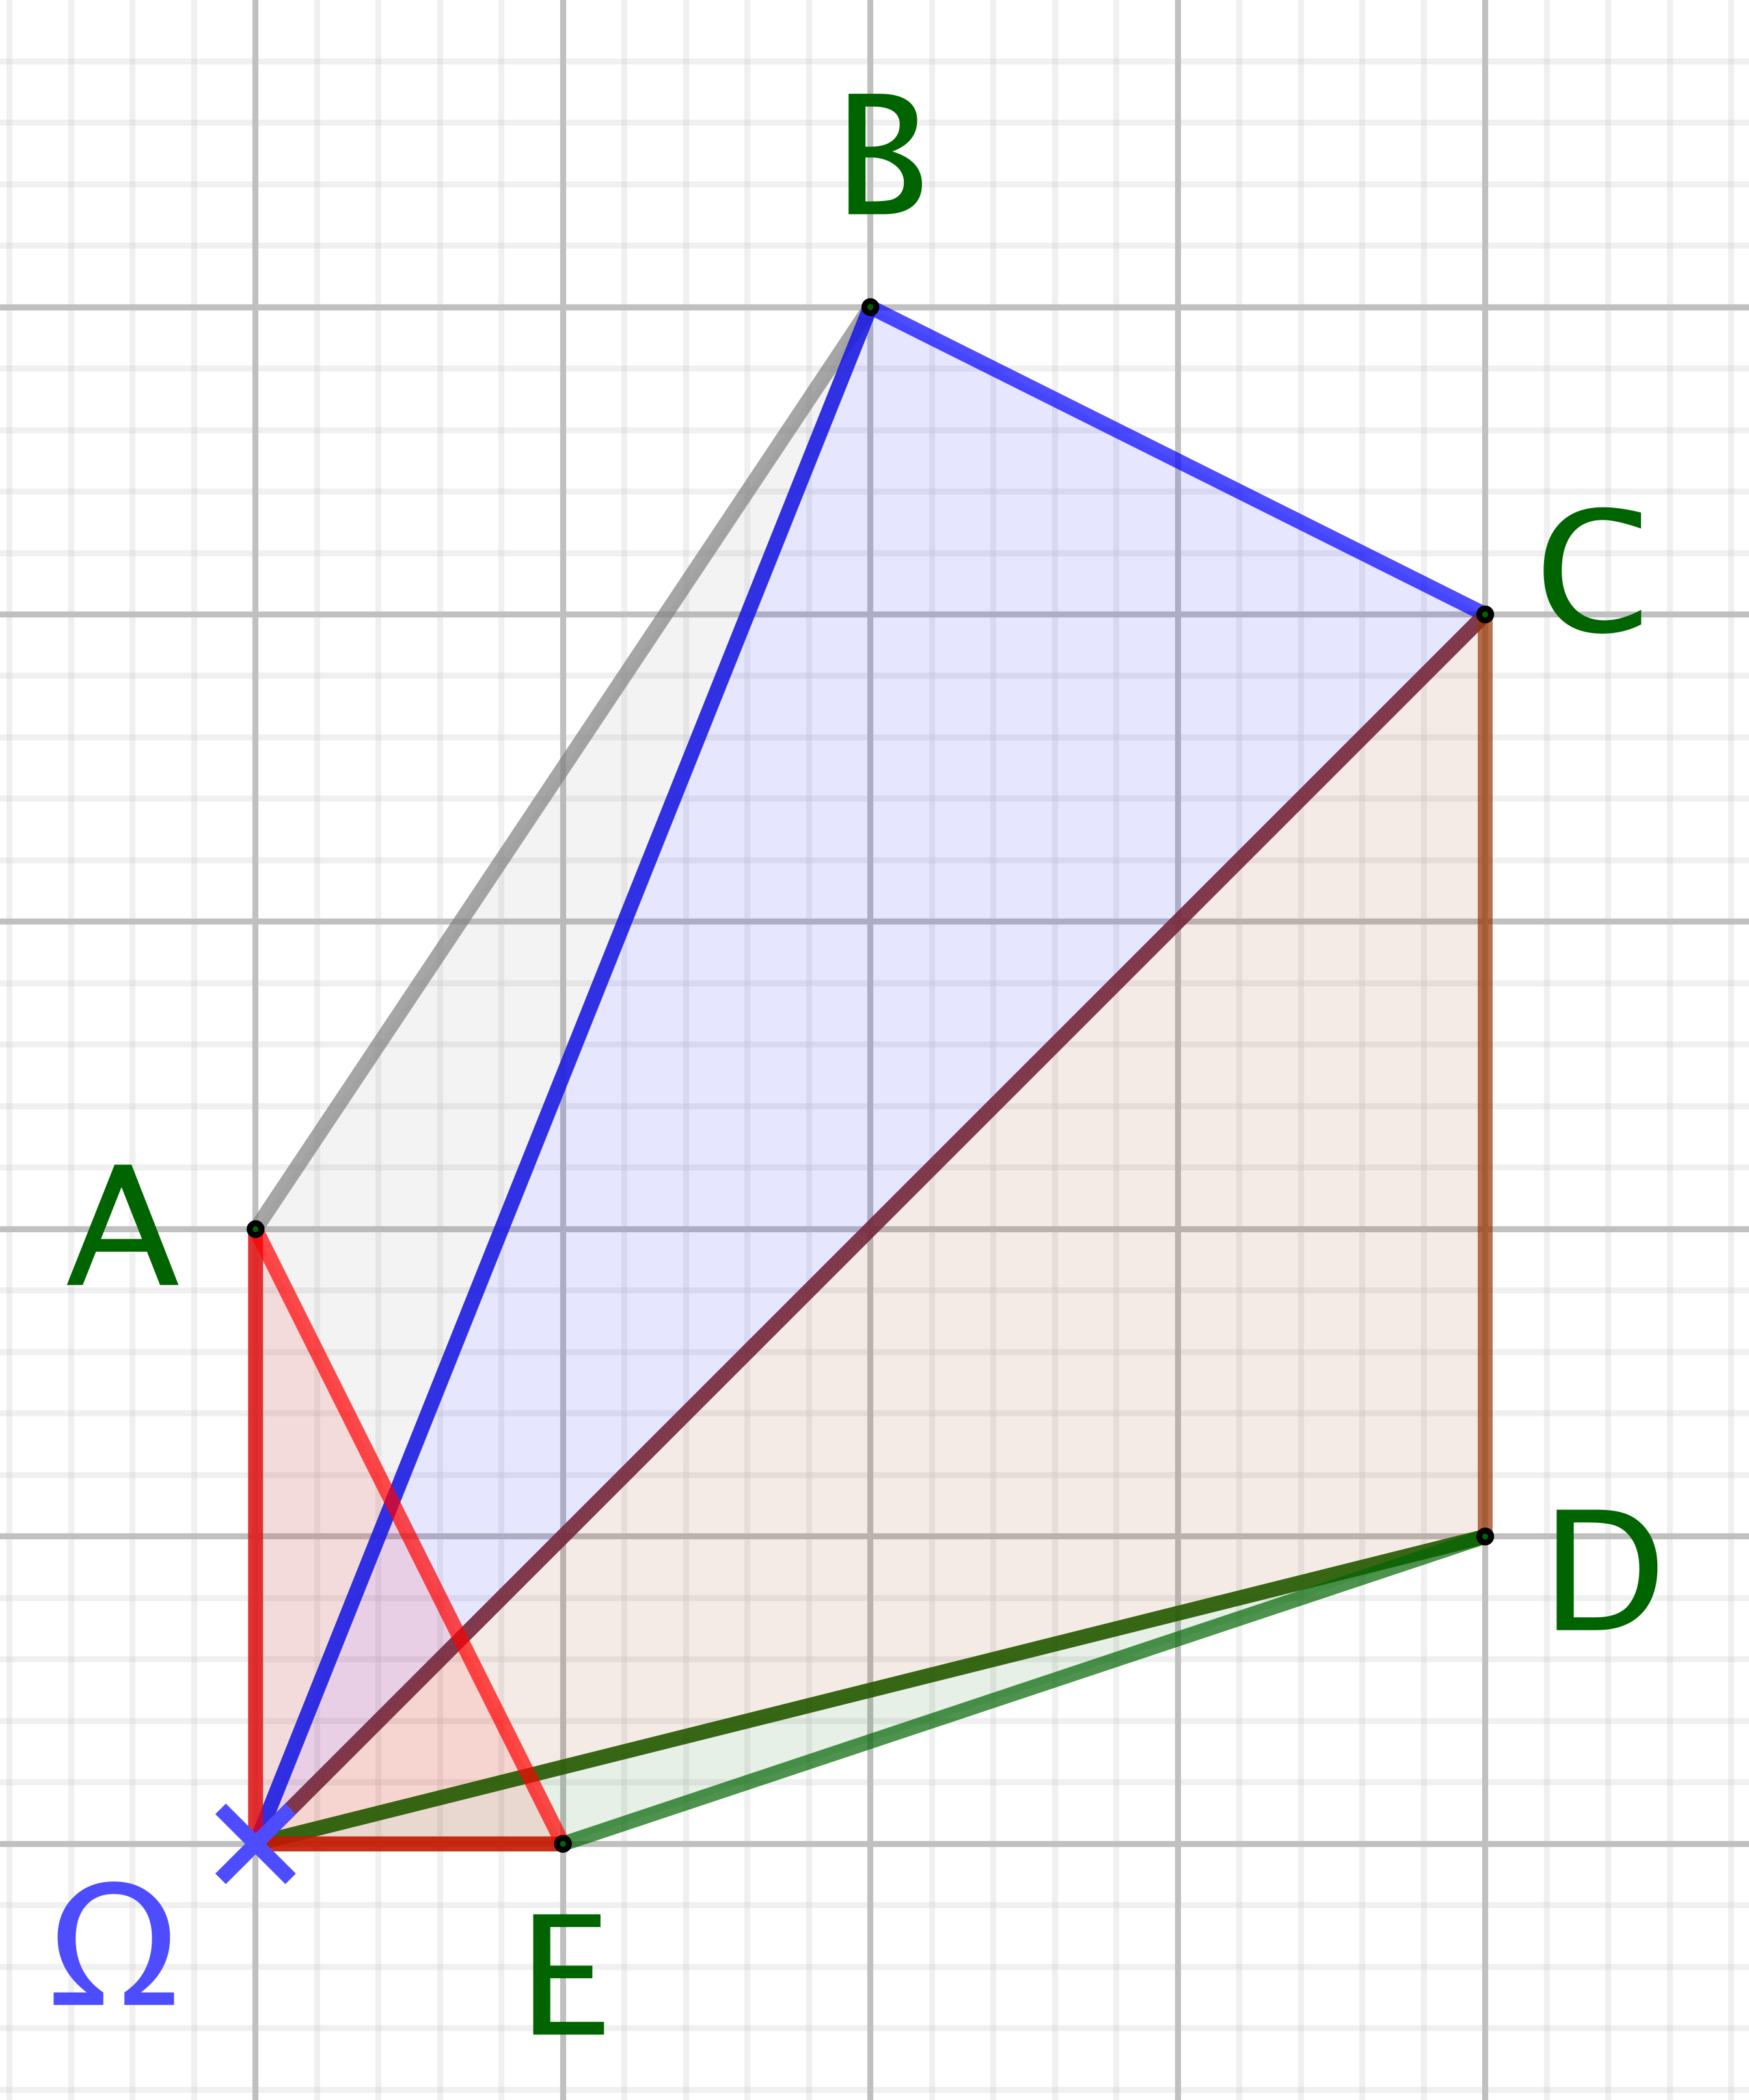
\includegraphics[scale=.4]{content/polygon/sufficient-cond/convex-2.png}
        
       	\smallskip
	
		$\num{14.5} = 2 + 7 + 4 + \num{4.5} - 4 \vphantom{\dfrac22}$
    \end{center}
\end{multicols}


Ce mode de calcul est celui employé par \geogebra\ qui donne une aire de \num{6.5} pour le polygone croisé de la bande dessinée ci-après qui détaille les calculs faits: les aires algébriques représentées en vert sont positives, et celles en rouge négatives.
Nous obtenons un total de $( - \num{6.5})$, soit la valeur fournie par \geogebra\ au signe près.

\newpage

\begin{multicols}{3}
    \small\itshape
    
    \begin{center}
        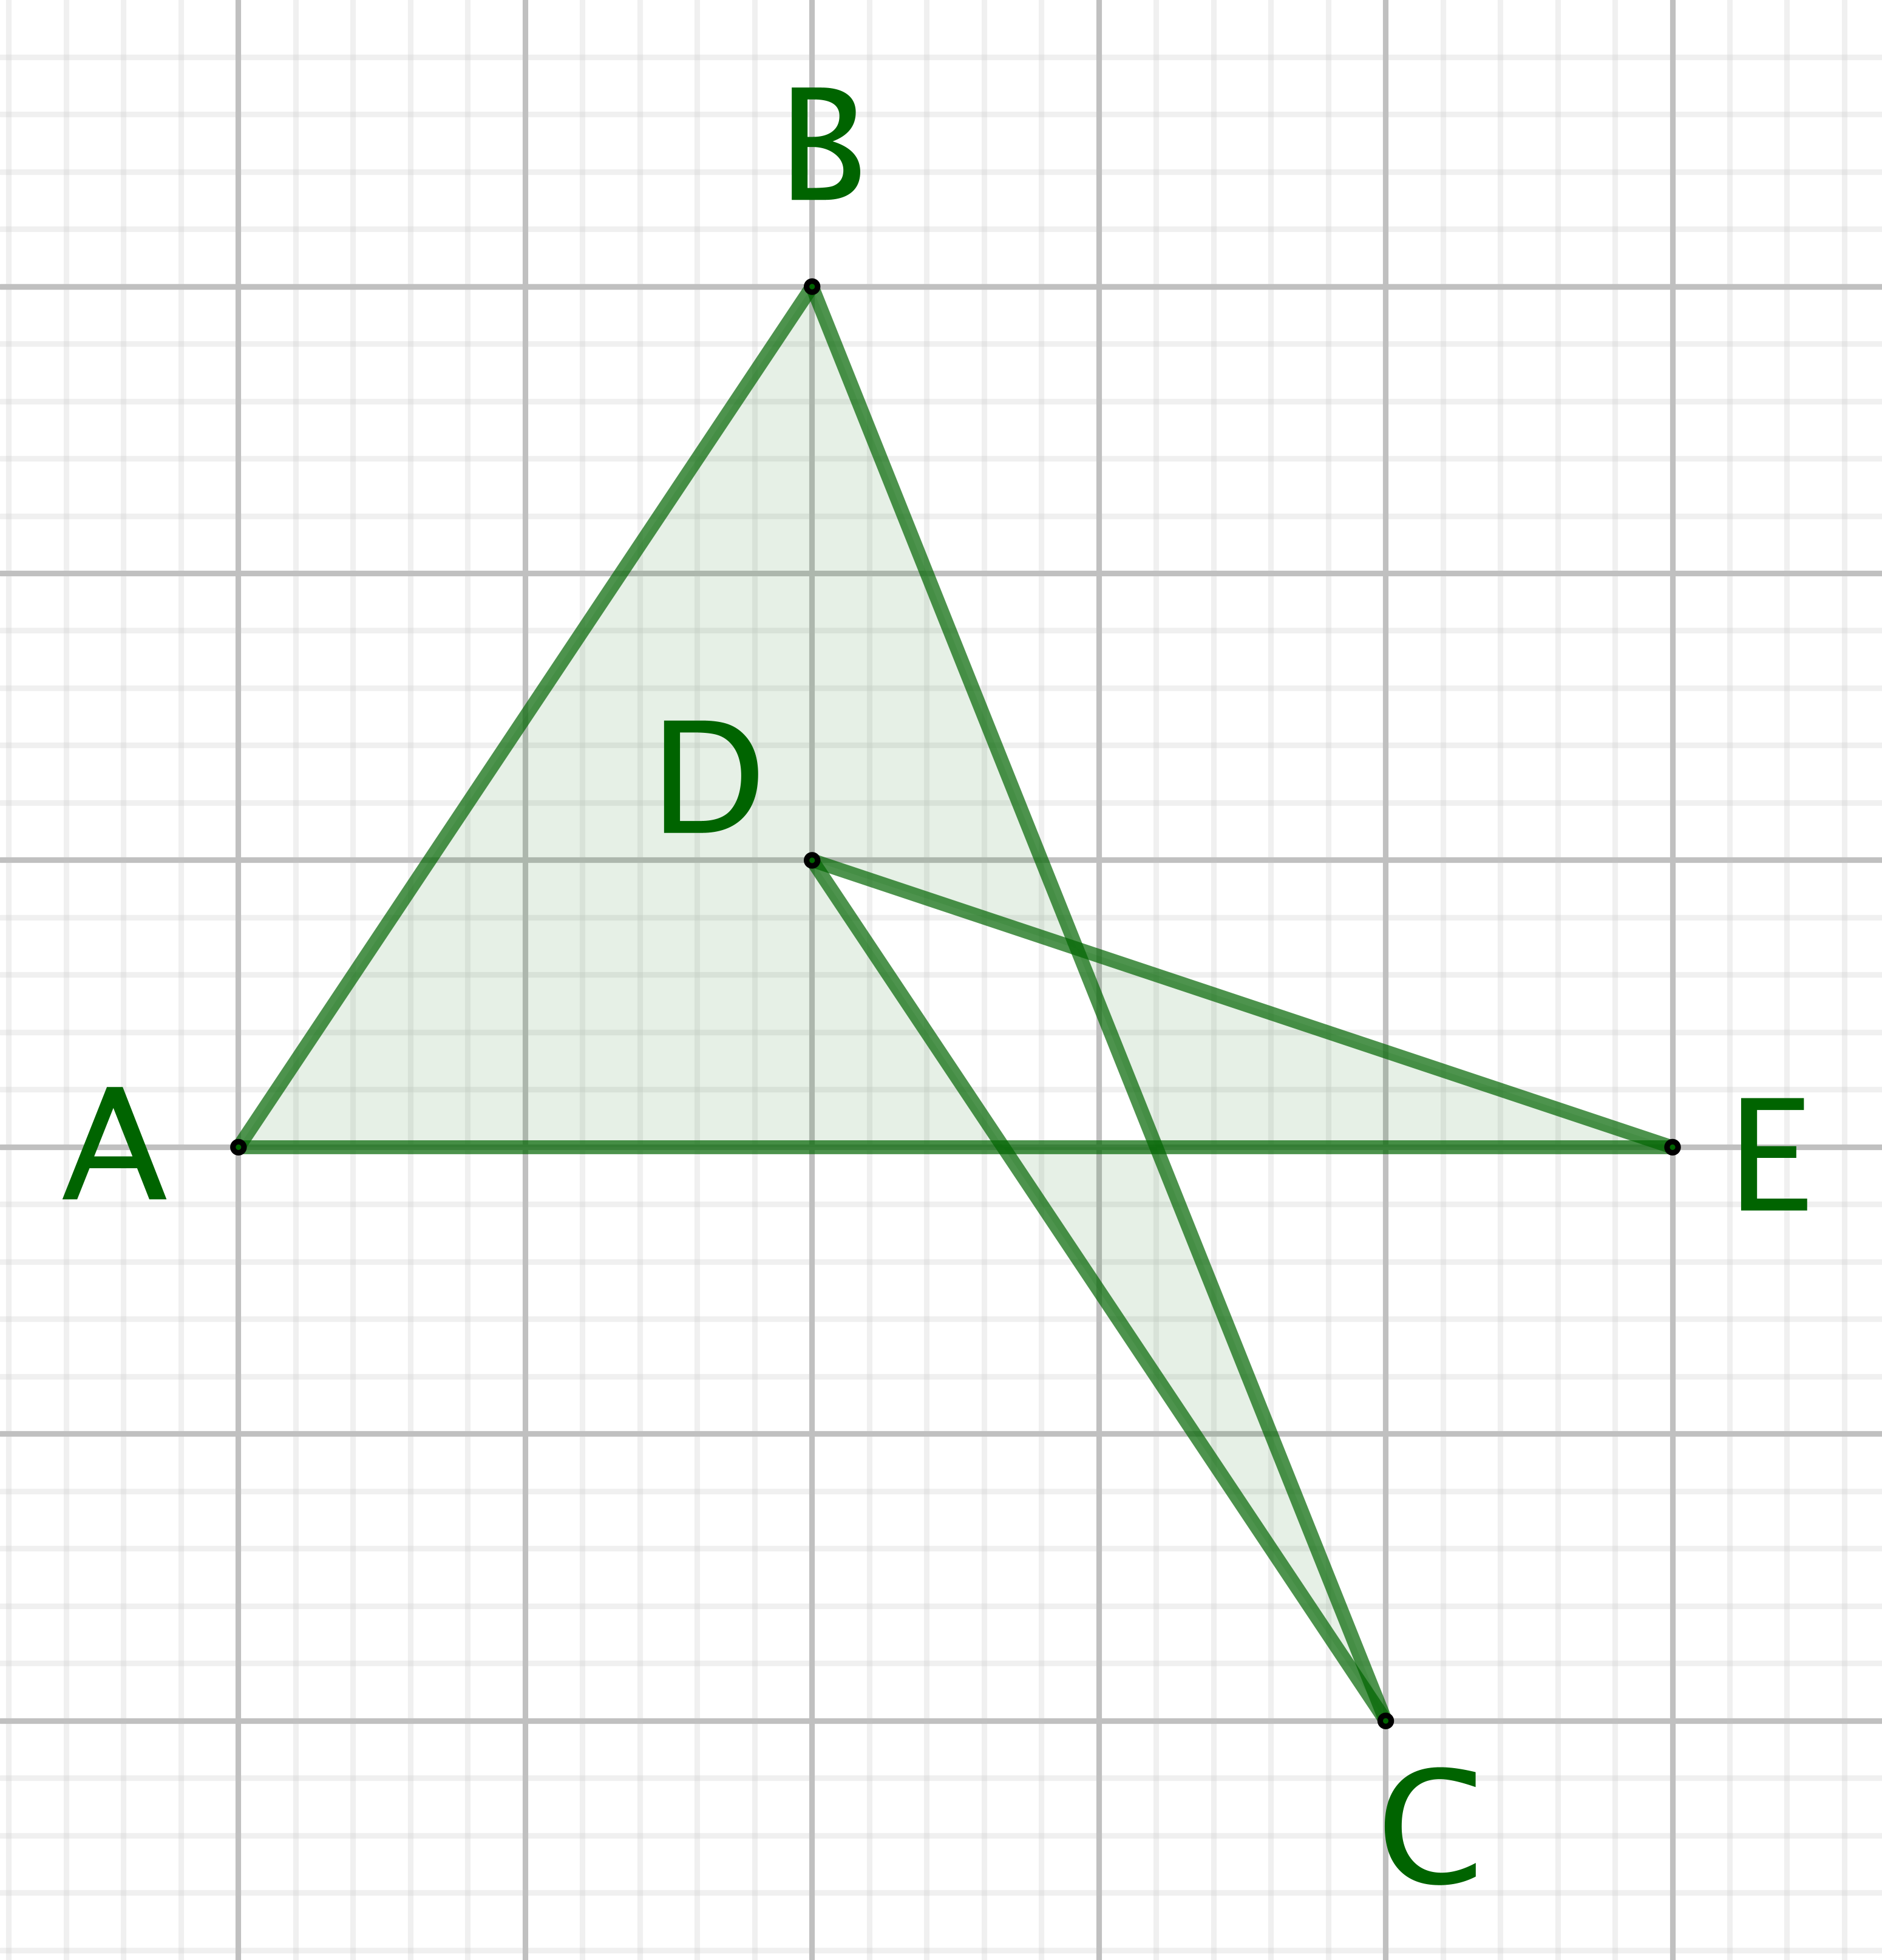
\includegraphics[scale=.4]{content/polygon/sufficient-cond/why.png}
    \end{center}
    
    \foreach \i in {3,1,4,2,5} {
    	\begin{center}
            \includegraphics[scale=.4]{content/polygon/sufficient-cond/why-step-\i.png}
        \end{center}
	}
\end{multicols}


Avant de formaliser ce qui précède, il faut noter que la notion d'aire algébrique est à manier avec prudence lorsqu'on la découvre. 
Si c'est votre cas, que pensez-vous de l'aire algébrique du quadrilatère croisé $ABCD$ ci-dessous qui est un antiparallélogramme très particulier? Réponse en note de bas de page.%
\footnote{
    La réponse est $0$. Comme nous verrons que le choix de $\Omega$ est libre, il suffit de faire les calculs avec $\Omega$ l'intersection des segments $[AD]$ et $[BC]$.
    On peut tout de même donner du sens à ceci. Voici comment. 
    Plongeons-nous dans l'espace. 
    Imaginons une toile rectangulaire rouge sur le dessus, et verte en dessous.
    Tournons de \qty{180}{\degree} verticalement l'un des côtés du rectangle.
    En supposant que la toile soit parfaitement tendue, nous obtenons, vue de dessus, un antiparallélogramme dont l'un des triangles est vert, et l'autre rouge.
    De façon savante, les deux faces ont deux orientations différentes. Nous reparlerons de cette notion par la suite.  
}

\begin{center}
    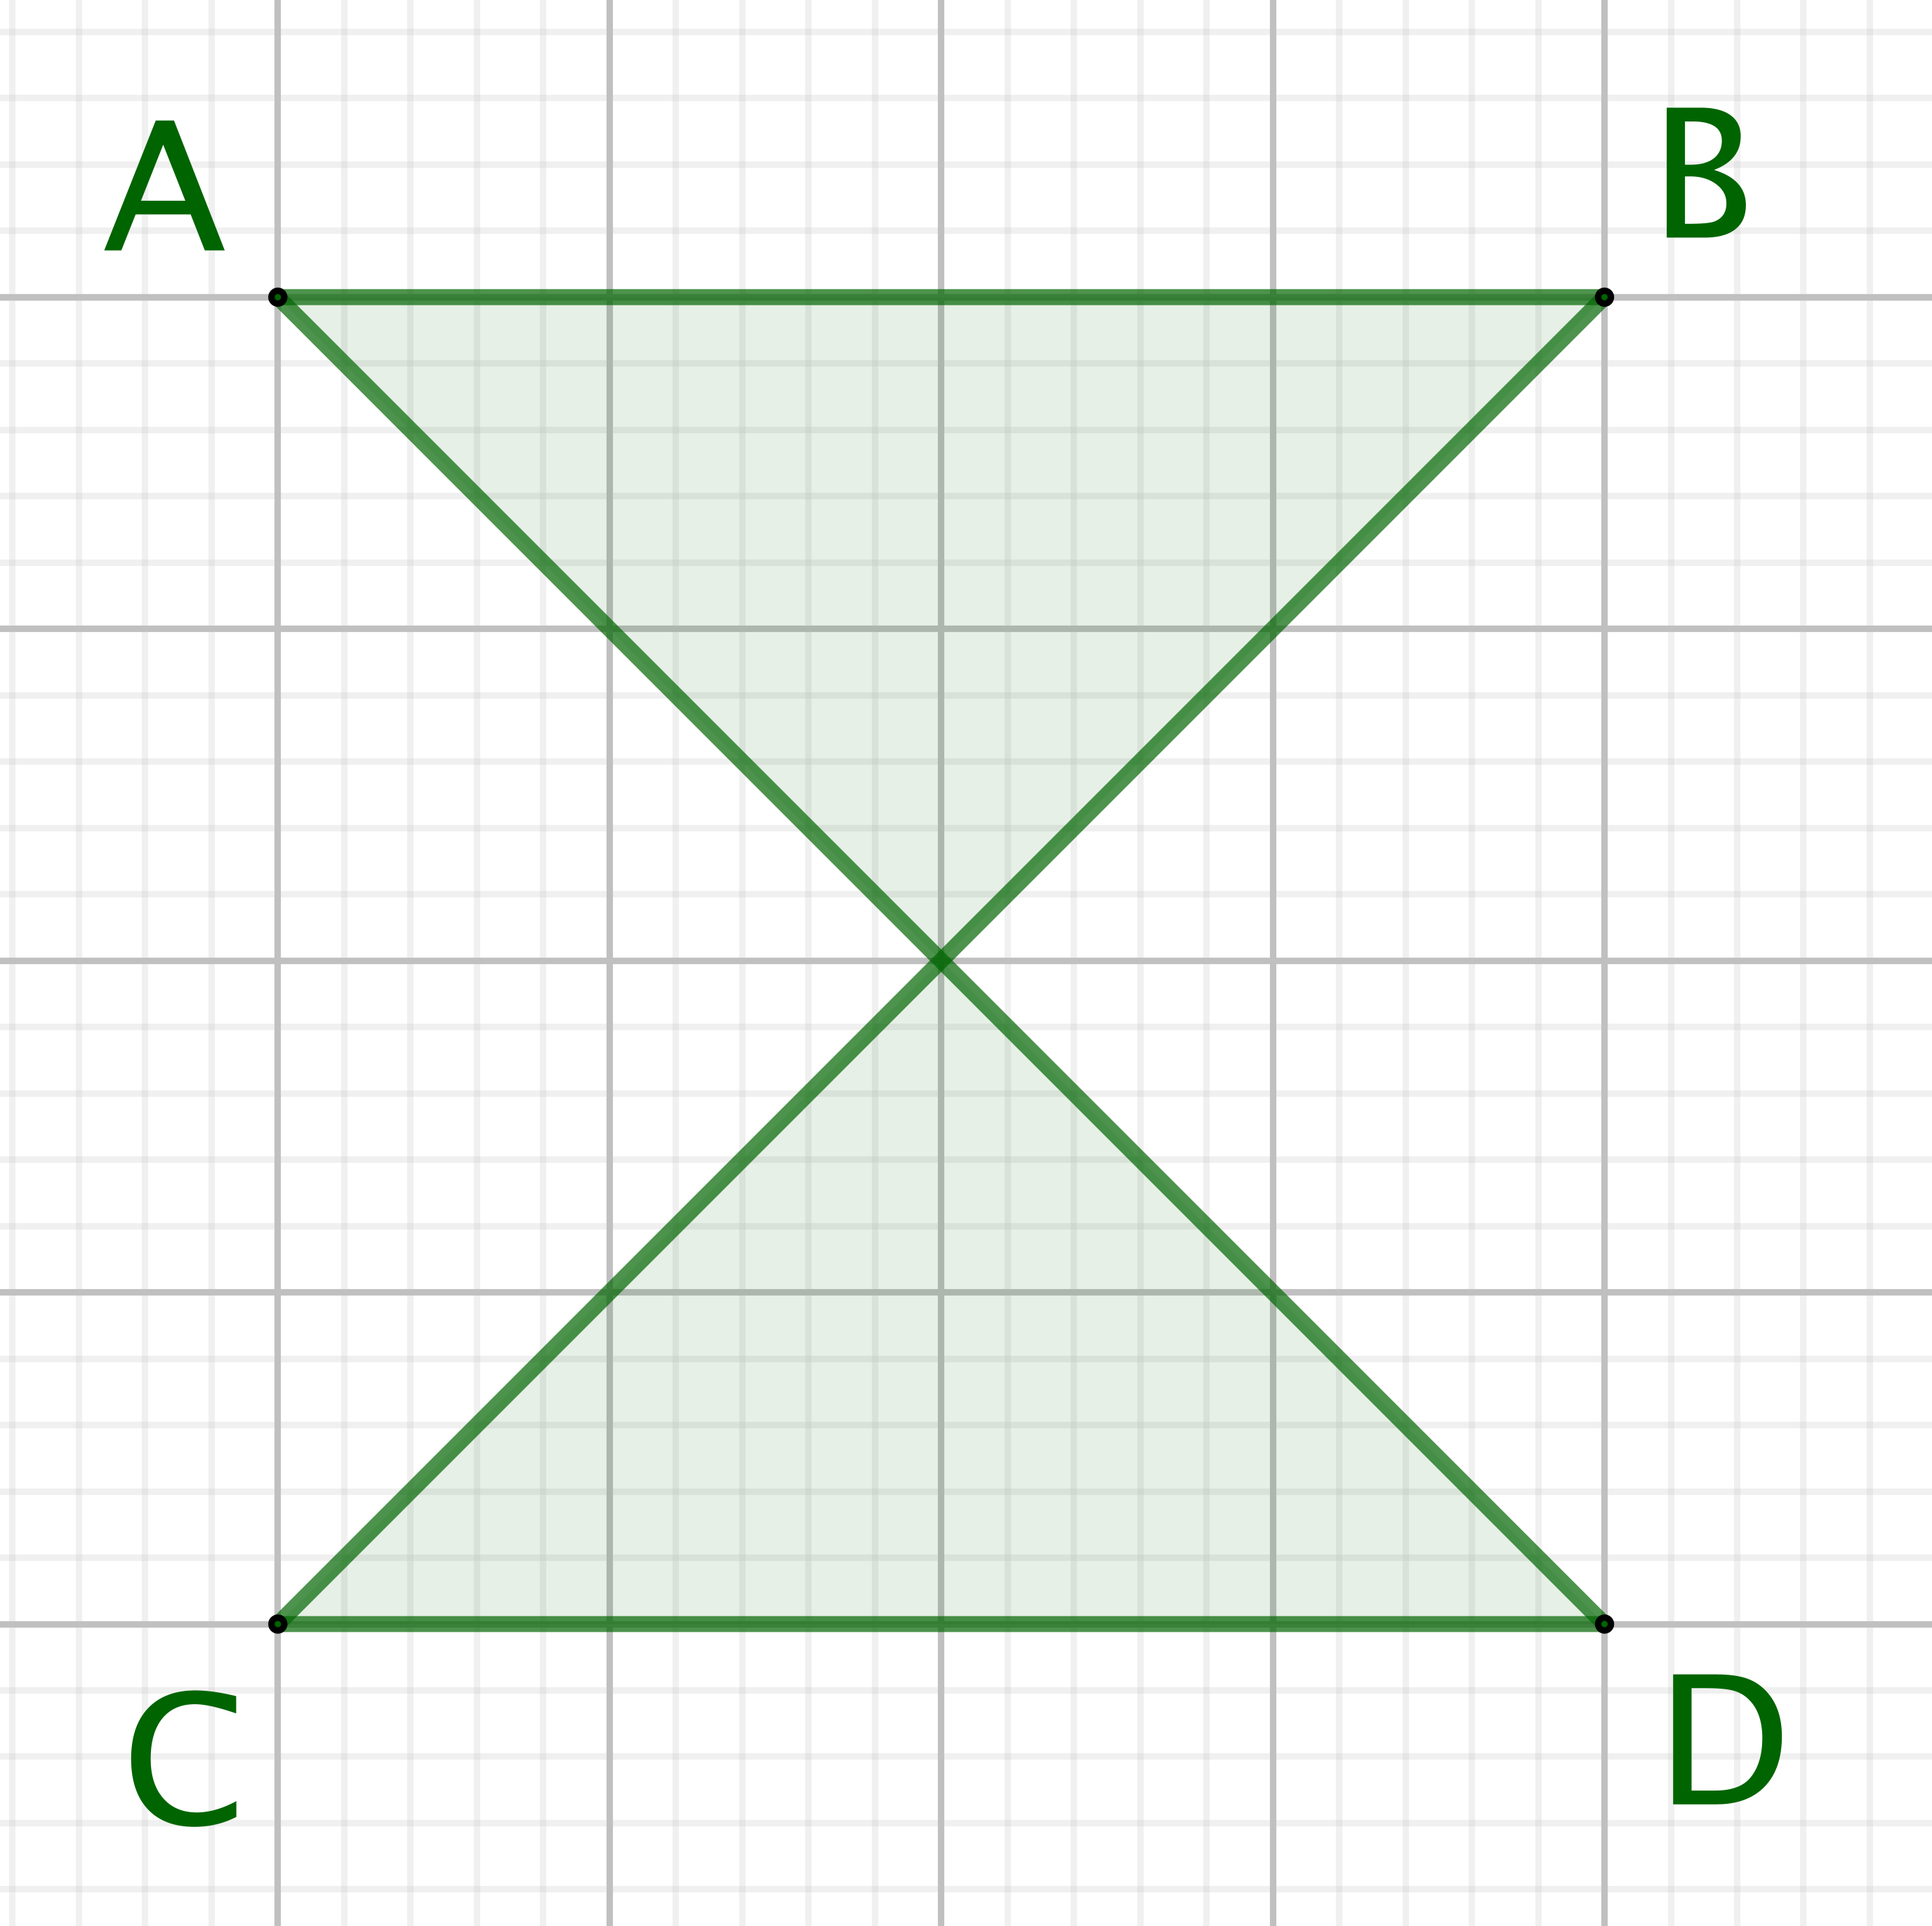
\includegraphics[scale=.4]{content/polygon/sufficient-cond/anti-para.png}
\end{center}


% ----------------------- %


\begin{defi} \label{garea-pt-ct}
    Pour toute \nline\  $\setproba{L} = A_1 A_2 \cdots A_n$, on définit $\big( A^{\,\prime}_i \big)_{i \in \ZZ}$ comme étant $n$-périodique, et vérifiant $A^{\,\prime}_{i} = A_i$ sur $\ZintervalC{1}{n}$.
\end{defi}


% ----------------------- %


\begin{fact} \label{garea-pt-ct}
    Soit $\setproba{L} = A_1 A_2 \cdots A_n$ une \nline.
    La fonction qui à un point $\Omega$ du plan associe 
    $\mu_1^n (\Omega ;\setproba{L}) = \dsum_{i=1}^{n} \det \big( \vect{\Omega A^{\,\prime}_i} , \vect{\Omega A^{\,\prime}_{i+1}} \big)$ est indépendante du point $\Omega$.
    Dans la suite, cette quantité indépendante de $\Omega$ sera notée $\mu_1^n (\setproba{L})$.
\end{fact}


\begin{proof}
    Soit $M$ un autre point du plan.

    \begin{stepcalc}[style=ar*]
        \mu_1^n (\Omega ;\setproba{L})
    \explnext{}
        \dsum_{i=1}^{n} \det \big( \vect{\Omega A^{\,\prime}_i} , \vect{\Omega A^{\,\prime}_{i+1}} \big)
    \explnext*{Cette bonne vieille relation de Chasles.}{}
        \dsum_{i=1}^{n} \det \big( \vect{\Omega M} + \vect{M A^{\,\prime}_i} , \vect{\Omega M} + \vect{M A^{\,\prime}_{i+1}} \big)
    \explnext{}
        \dsum_{i=1}^{n} \Big[
            \det \big( \vect{\Omega M} , \vect{\Omega M} \big)
            +
            \det \big( \vect{\Omega M} , \vect{M A^{\,\prime}_{i+1}} \big)
            +
            \det \big( \vect{M A^{\,\prime}_i} , \vect{\Omega M} \big)
            +
            \det \big( \vect{M A^{\,\prime}_i} , \vect{M A^{\,\prime}_{i+1}} \big)
        \Big]
    \explnext{}
        \dsum_{i=1}^{n} \det \big( \vect{\Omega M} , \vect{M A^{\,\prime}_{i+1}} \big)
        +
        \dsum_{i=1}^{n} \det \big( \vect{M A^{\,\prime}_i} , \vect{\Omega M} \big)
        +
        \mu_1^n (M ; \setproba{L})
    \explnext{}
        \mu_1^n (M ; \setproba{L})
        +
        \dsum_{i=2}^{n+1} \det \big( \vect{\Omega M} , \vect{M A^{\,\prime}_{i}} \big)
        -
        \dsum_{i=1}^{n} \det \big( \vect{\Omega M} , \vect{M A^{\,\prime}_i} \big)
    \explnext{}
        \mu_1^n (M ; \setproba{L})
        +
        \det \big( \vect{\Omega M} , \vect{M A^{\,\prime}_{n+1}} \big)
        -
        \det \big( \vect{\Omega M} , \vect{M A^{\,\prime}_1} \big)
    \explnext*{$A^{\,\prime}_{n+1} = A^{\,\prime}_1$}{}
        \mu_1^n (M ; \setproba{L})
    \end{stepcalc}
    
    \null\vspace{-3.5ex}
\end{proof}
    
    
% ----------------------- %


\begin{fact} \label{nline-shift-inva}
    Soit $\setproba{L} = A_1 A_2 \cdots A_n$ une \nline.
    Pour $k \in \ZintervalC{1}{n}$, 
    la \nline\ $\setproba{L}_j = B_1 B_2 \cdots B_n$, où $B_i = A^{\,\prime}_{k+i-1}$,
    vérifie
    $\mu_1^n (\setproba{L}) = \mu_1^n (\setproba{L}_k)$.
    Dans la suite, cette quantité commune sera notée $\mu (\setproba{L})$.
\end{fact}


\begin{proof}
    Il suffit de s'adonner à un petit jeu sur les indices de sommation.
\end{proof}
    
    
% ----------------------- %


\begin{fact} \label{nline-rota-inva}
    Soit 
    $\setproba{L} = A_1 A_2 \cdots A_n$ une \nline. 
    La \nline\ $\setproba{L}^{\mathrm{op}} = B_1 B_2 \cdots B_n$, où $B_i =  A_{n + 1 - i}$,
    vérifie
    $\mu(\setproba{L}^{\mathrm{op}}) = {} - \mu(\setproba{L})$.
\end{fact}


\begin{proof}
    Soit $\Omega$ un point quelconque du plan.

    \begin{stepcalc}[style=ar*]
        \mu(\setproba{L}^{\mathrm{op}})
    \explnext{}
        \dsum_{i=1}^{n} \det \big( \vect{\Omega B^{\,\prime}_i} , \vect{\Omega B^{\,\prime}_{i+1}} \big)
    \explnext{}
        \dsum_{i=1}^{n} \det \big( \vect{\Omega A^{\,\prime}_{n + 1 - i}} , \vect{\Omega A^{\,\prime}_{n - i}} \big)
    \explnext{}
        \dsum_{j=0}^{n-1} \det \big( \vect{\Omega A^{\,\prime}_{j + 1}} , \vect{\Omega A^{\,\prime}_j} \big)
    \explnext*{$A^{\,\prime}_0 = A^{\,\prime}_n$ et $A^{\,\prime}_1 = A^{\,\prime}_{n+1}$}{}
        \dsum_{j=1}^{n} \det \big( \vect{\Omega A^{\,\prime}_{j + 1}} , \vect{\Omega A^{\,\prime}_j} \big)
    \explnext{}
        {} - \dsum_{j=1}^{n} \det \big( \vect{\Omega A^{\,\prime}_j} ,  \vect{\Omega A^{\,\prime}_{j + 1}} \big)
    \explnext{}
        {} - \mu(\setproba{L})
    \end{stepcalc}
    
    \null\vspace{-3.5ex}
\end{proof}
    
    
% ----------------------- %


\begin{fact}
    Soit 
    $\setproba{L} = A_1 A_2 \cdots A_n$ une \nline.
    La quantité $\frac12 \abs{\mu(\setproba{L})}$ ne dépend ni du sens de parcours de $\setproba{L}$, ni du point de départ choisi.%
    \footnote{
        Le lecteur pardonnera les abus de langage utilisés.
    }
    Elle sera notée $\garea{\setproba{L}}$, et nommée \og \emph{aire généralisée} \fg\ de la \nline\ $\setproba{L}$.
\end{fact}


\begin{proof}
    C'est une synthèse des faits \ref{nline-shift-inva} et \ref{nline-rota-inva}.
\end{proof}
    
    
% ----------------------- %


Pour notre démonstration finale, nous aurons besoin de savoir que $\garea{\setproba{P}} = \area{\setproba{P}}$ pour tout \ngone\ $\setproba{P}$.%
\footnote{
	Nous obtenons ainsi la généralisation de l'aire géométrique usuelle au cas des polygones croisés.
}
Ceci est évident dans le cas convexe, car il suffit de choisir l'isobarycentre $G$ de $A_1$, $A_2$, ..., $A_n$ pour le calcul de $\garea{\setproba{P}}$: en effet, avec ce choix, tous les déterminants $\det \big( \vect{G A^{\,\prime}_i} , \vect{G A^{\,\prime}_{i+1}} \big)$ ont le même signe.
Dans le cas non-convexe, les choses se compliquent, car nous ne maîtrisons plus les signes des déterminants. 



???
La présence de la valeur absolue nous demande de connaître mieux le signe

    
    
% ----------------------- %


\begin{fact}
    Pour tout \ngone\ $\setproba{P}$, nous avons: $\garea{\setproba{P}} = \area{\setproba{P}}$.
\end{fact}


\begin{proof}
    Le théorème de triangulation affirme que tout \ngone\ est triangulable comme dans l'exemple très basique suivant qui laisse envisager une démonstration par récurrence en retirant l'un des triangles ayant deux côtés correspondant à deux côtés consécutifs du \ngone\ (pour peu qu'un tel triangle existe toujours).

    
    \begin{multicols}{3}
        \small\itshape
        \begin{center}
            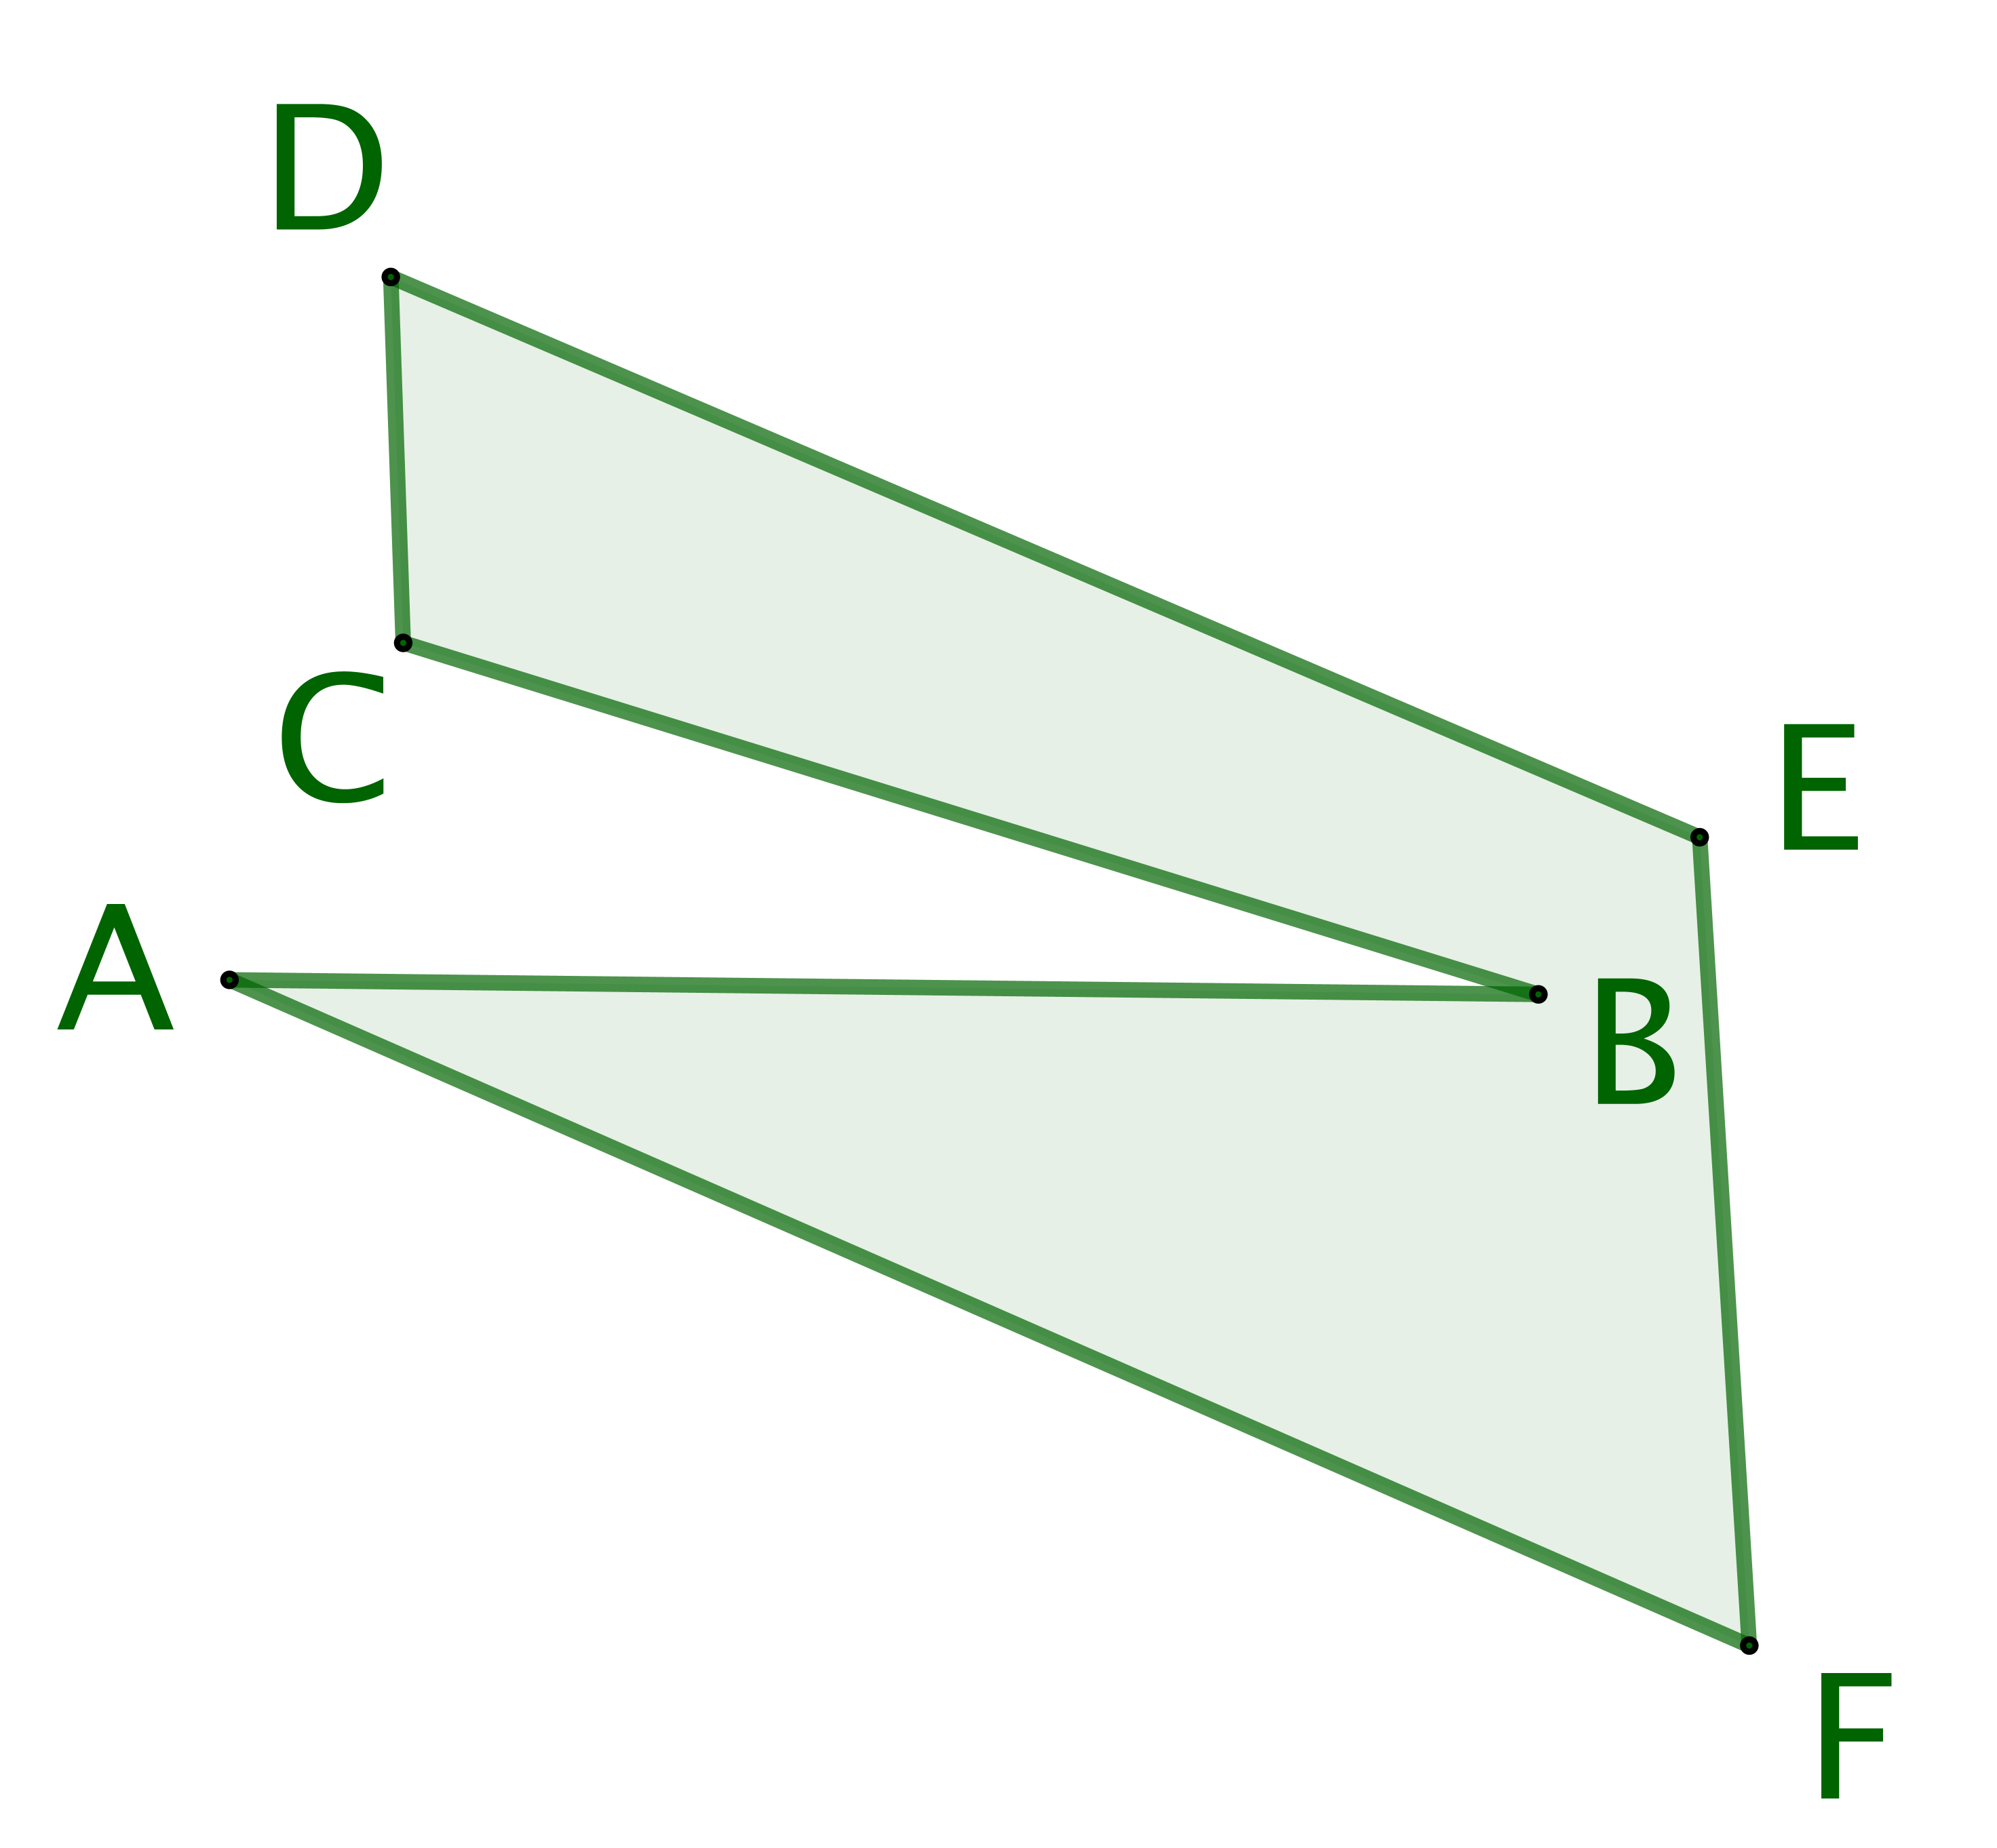
\includegraphics[scale=.4]{content/polygon/sufficient-cond/triangulation-1.png}
        
            \smallskip
            Un \ngone\ nu.
        \end{center}

    
        \begin{center}
            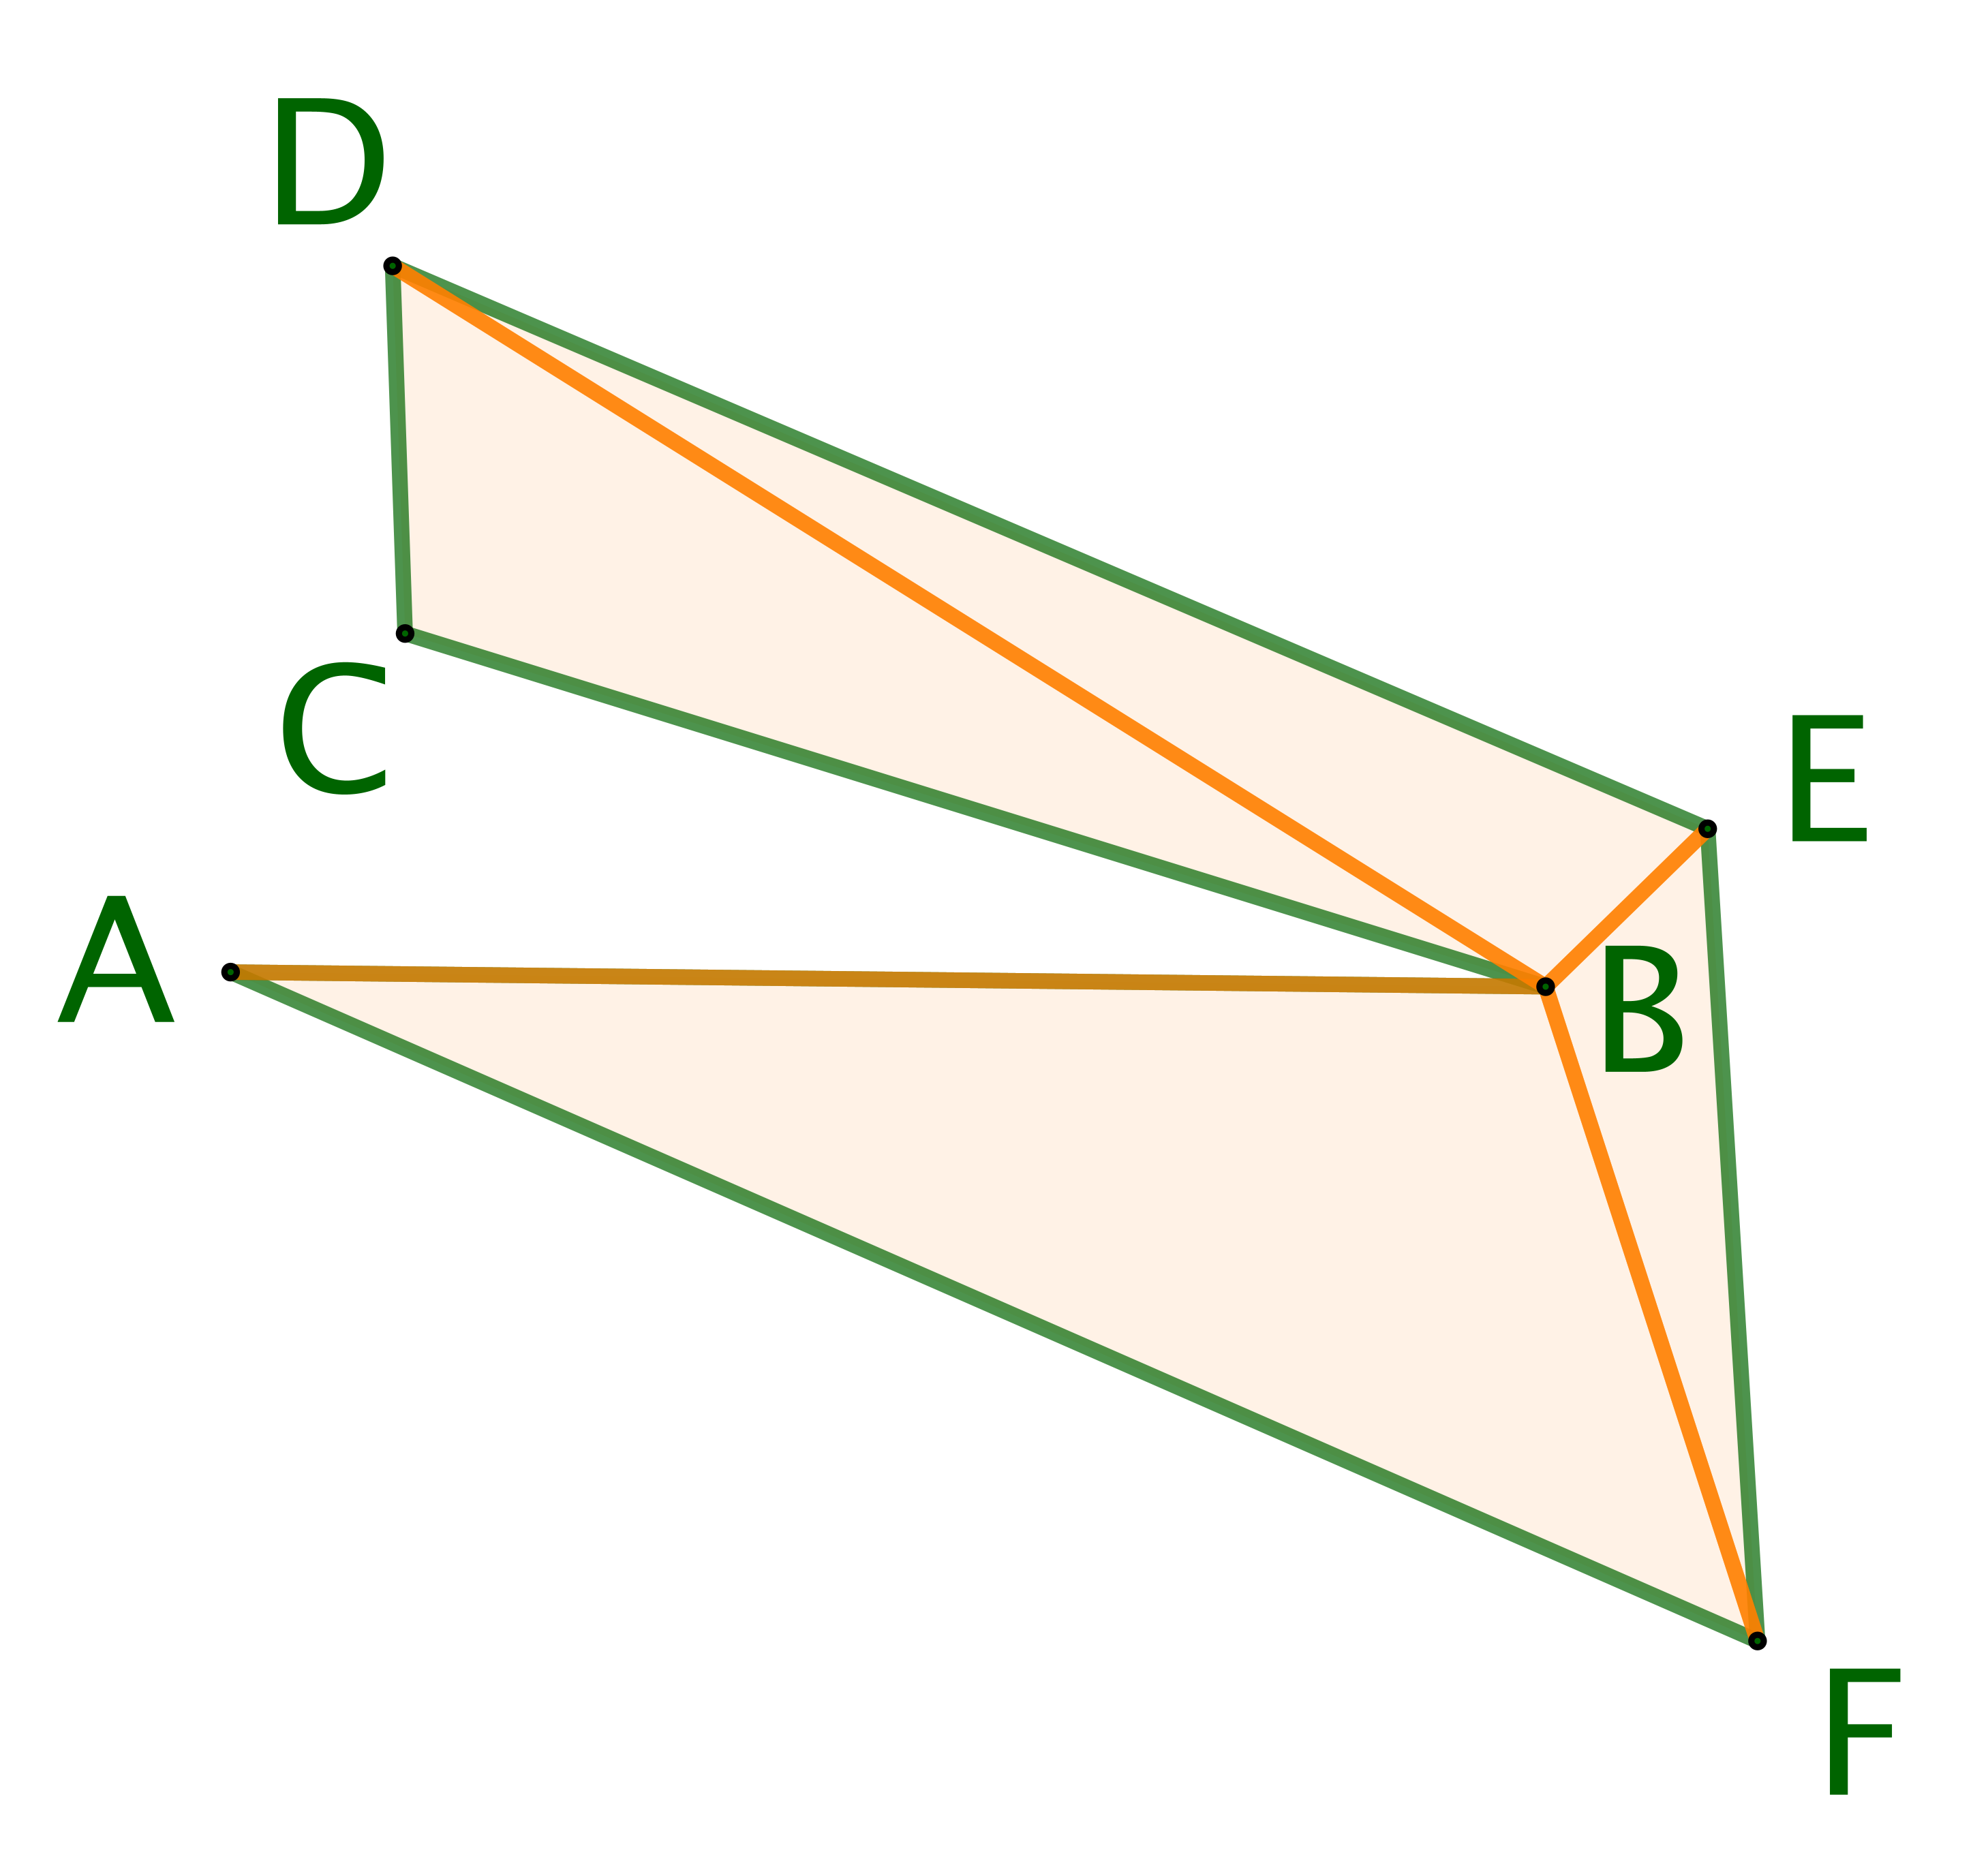
\includegraphics[scale=.4]{content/polygon/sufficient-cond/triangulation-2.png}
        
            \smallskip
            Le \ngone\ triangulé.
        \end{center}

    
        \begin{center}
            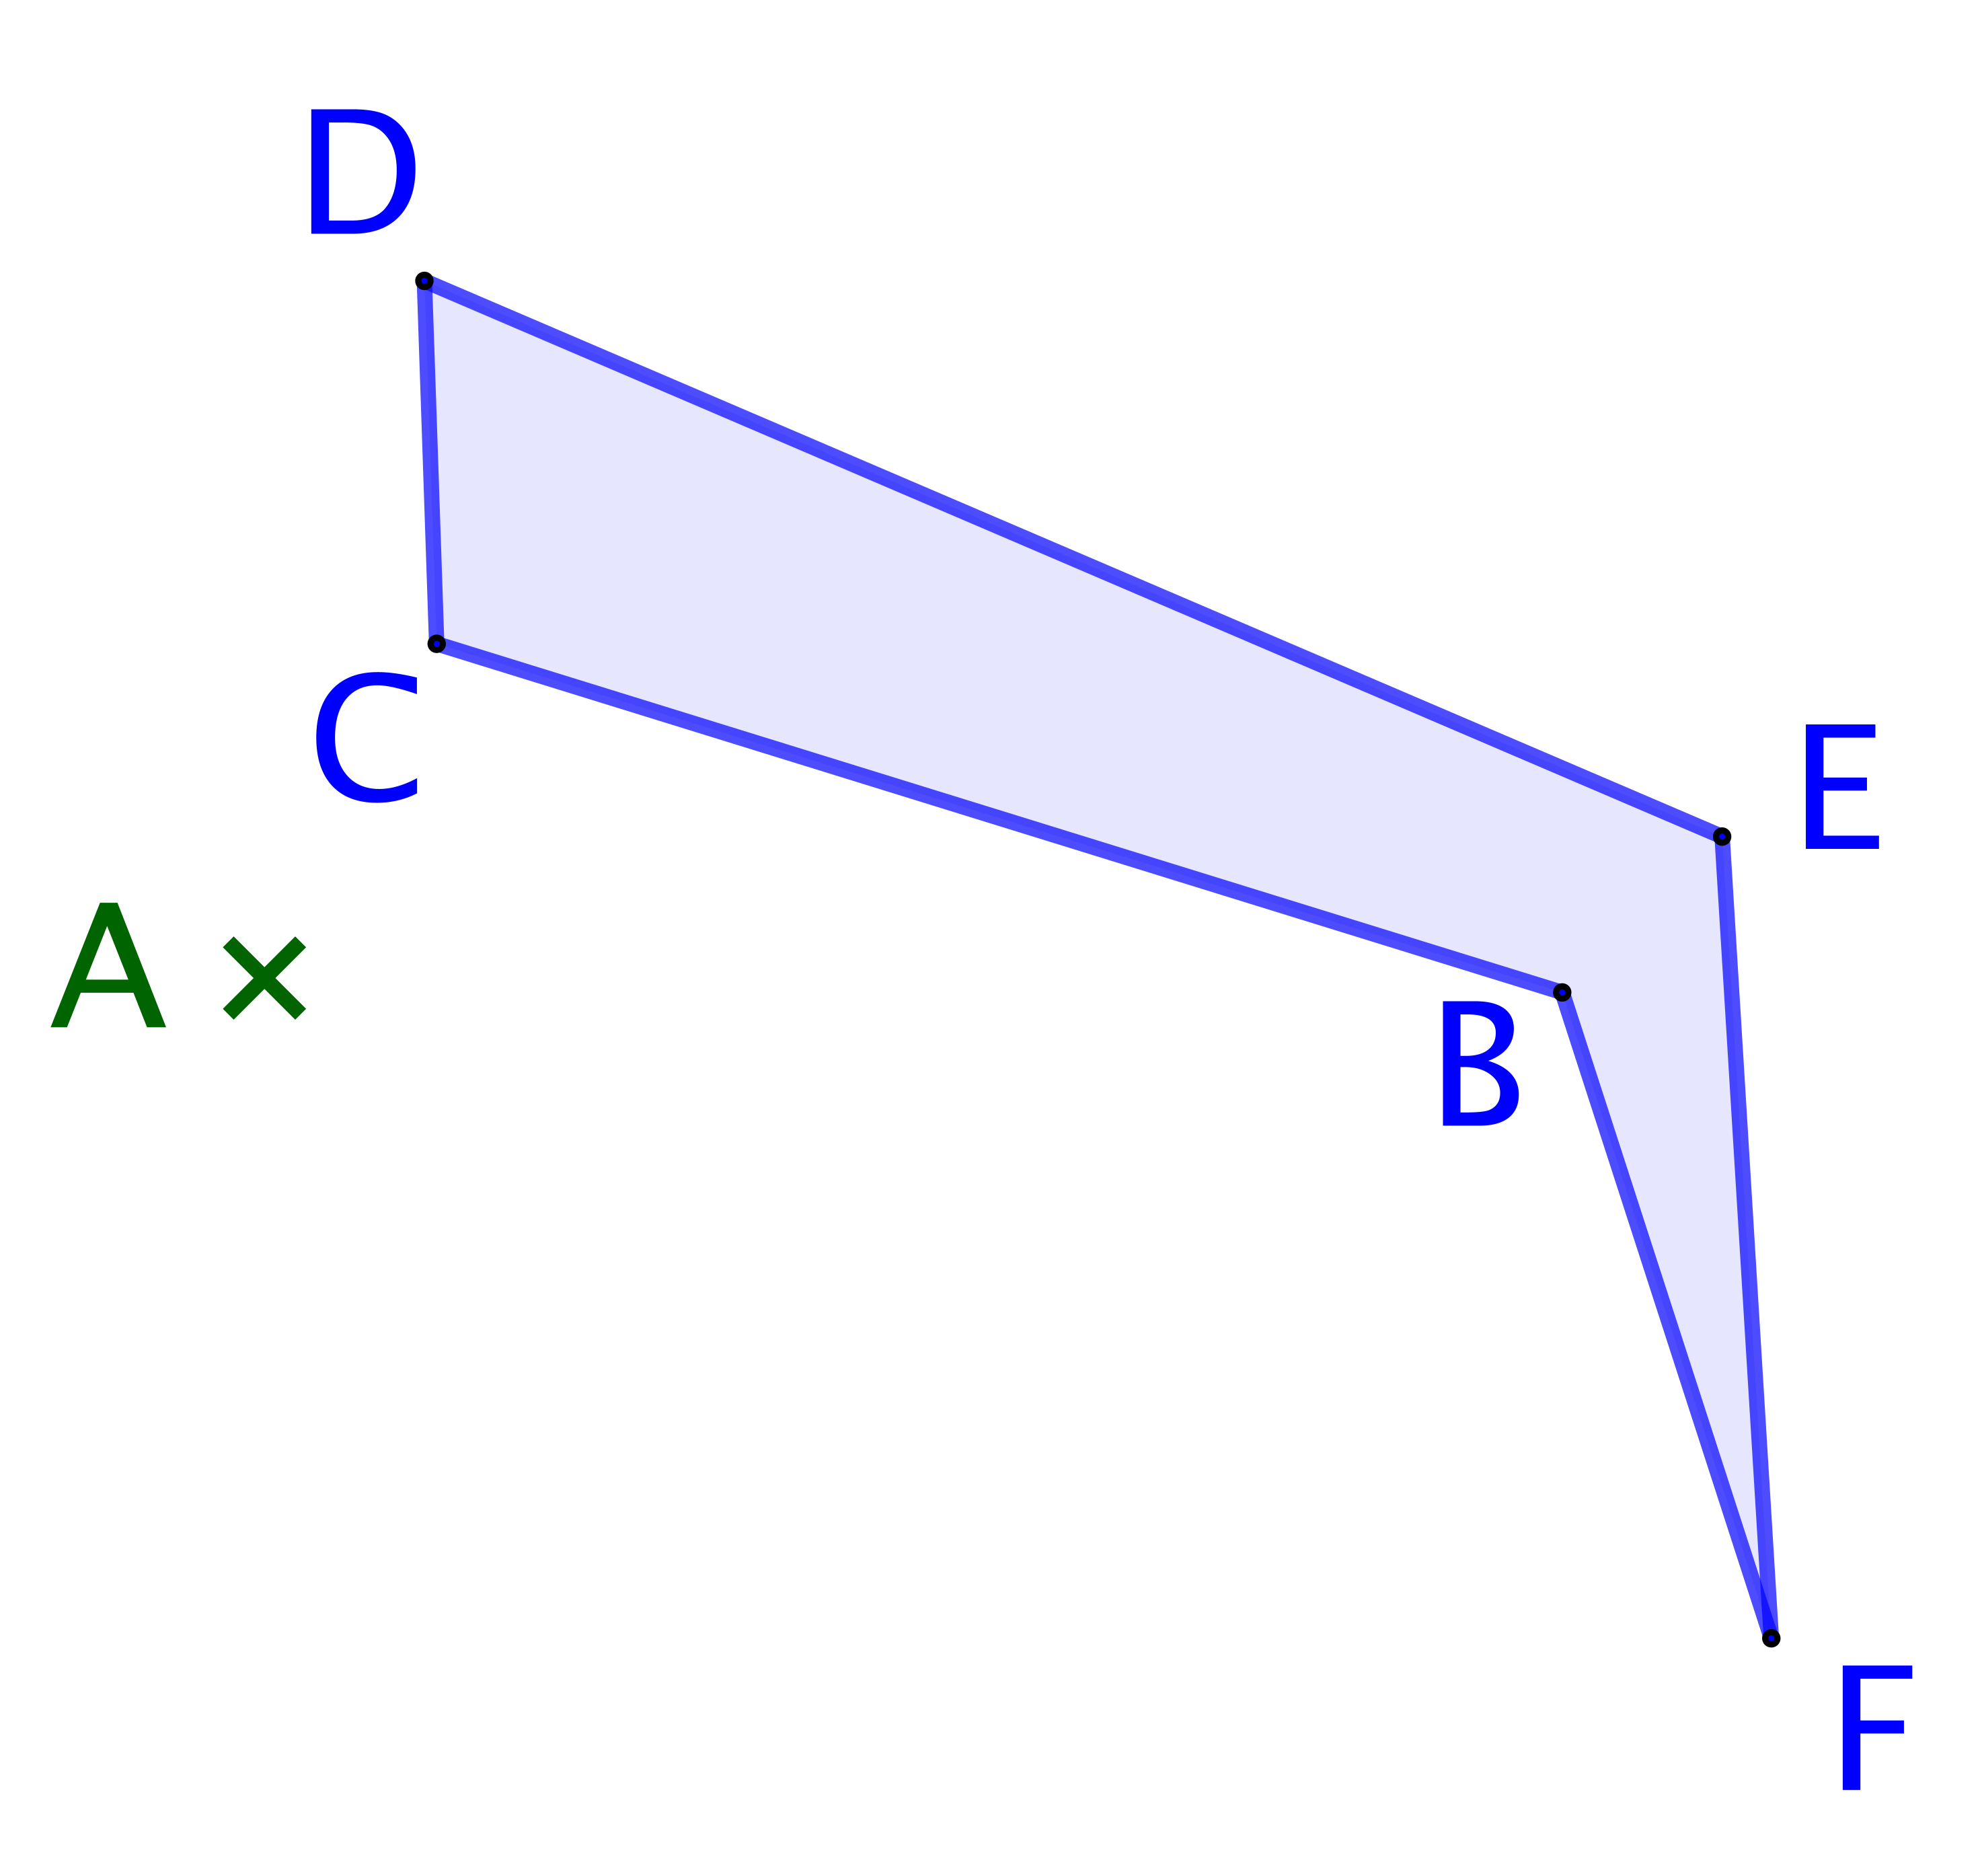
\includegraphics[scale=.4]{content/polygon/sufficient-cond/triangulation-3.png}
        
            \smallskip
            Le \ngone\ allégé.
        \end{center}
    \end{multicols}
    
    
    Le théorème de triangulation admet une forme forte donnant une décomposition contenant un triangle formé de deux côtés consécutifs du \ngone.%
    \footnote{
        En pratique, cette forme forte est peu utile, car elle aboutit à un algorithme de recherche trop lent.
    }
    Nous dirons qu'une telle décomposition est \og \emph{à l'écoute} \fg.
    Ce très mauvais jeu de mots fait référence à la notion sérieuse \og \emph{d'oreille} \fg\ pour un \ngone: une oreille est un triangle inclus dans le \ngone, et formé de deux côtés consécutifs du \ngone.
    L'exemple suivant donne un \ngone\ n'ayant que deux oreilles: ceci montre que l'existence d'une oreille ne va pas de soi.%
    \footnote{
        On démontre que tout \ngone\ admet au minimum deux oreilles.
    }


    \begin{multicols}{2}
        \small\itshape
    	\begin{center}
        	
\includegraphics[scale=.4]{content/polygon/sufficient-cond/mini-ear-1.png}
        
        	\smallskip
       		Un \ngone\ basique.
    	\end{center}
	
    	\begin{center}
        	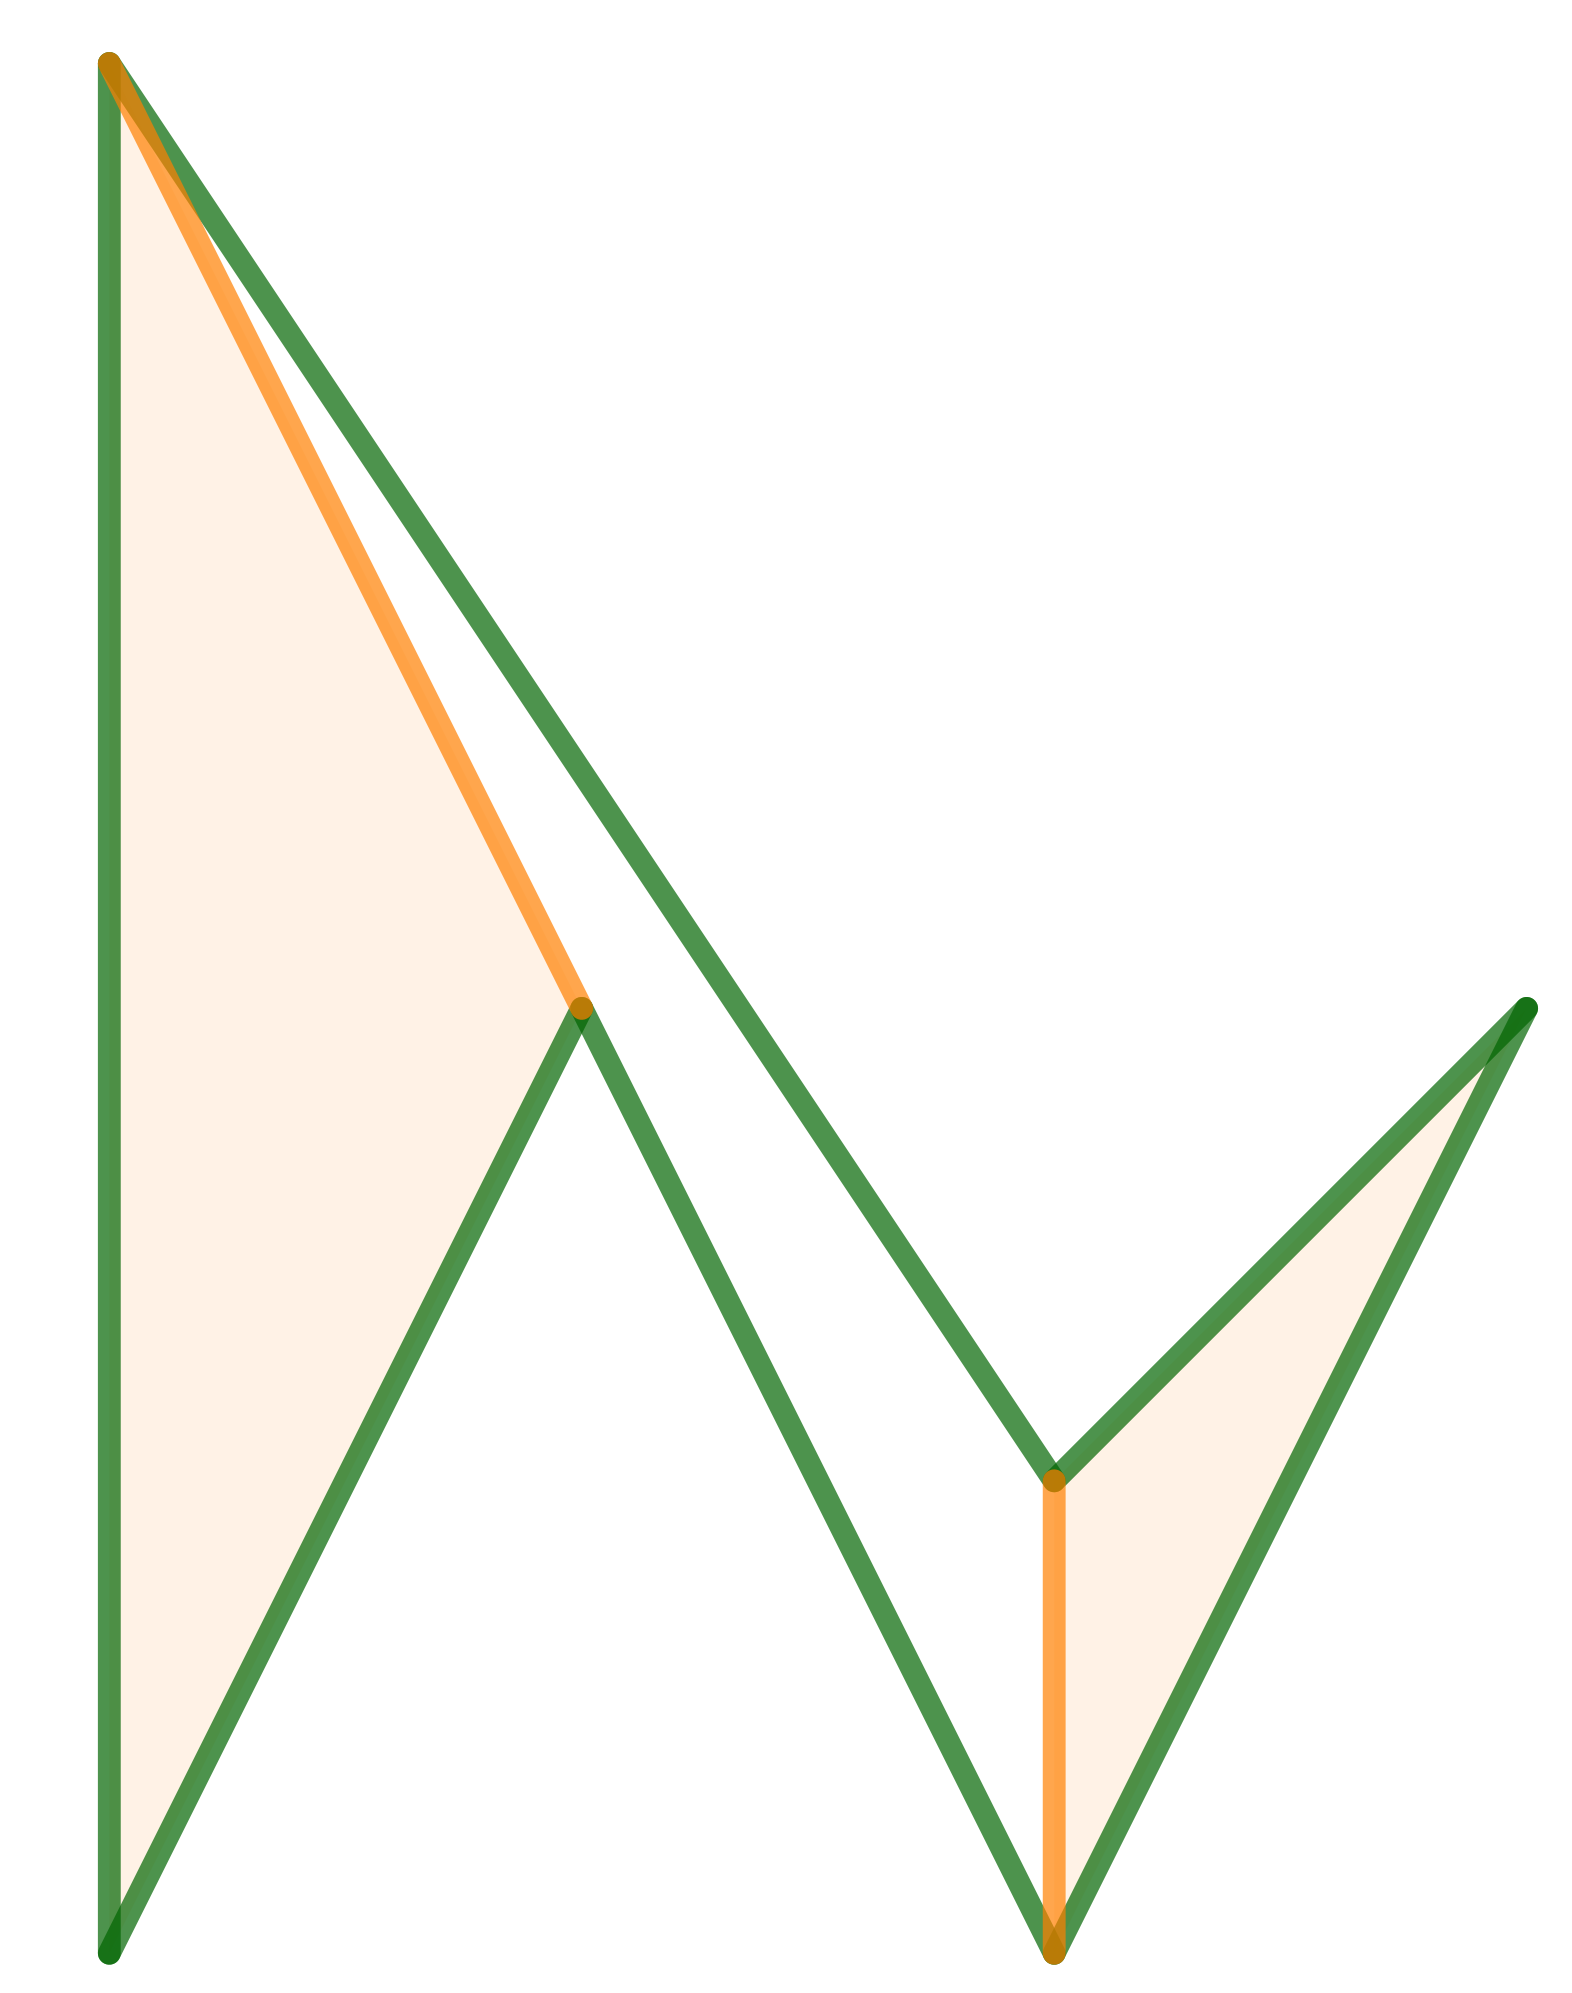
\includegraphics[scale=.4]{content/polygon/sufficient-cond/mini-ear-2.png}
        
        	\smallskip
       		Juste deux oreilles disponibles.
    	\end{center}
    \end{multicols}
    
    
    
    Soit $\setproba{P}$ un \ngone\ avec $n \geq 4$, et $\setproba{L} = A_1 A_2 \cdots A_n$ la \nline\ obtenue en parcourant la frontière de $\setproba{P}$ à partir d'un sommet $A_1$ tel que $A_1 A_{n-1} A_n$ soit une oreille de $\setproba{P}$.
    
    
    \begin{center}
        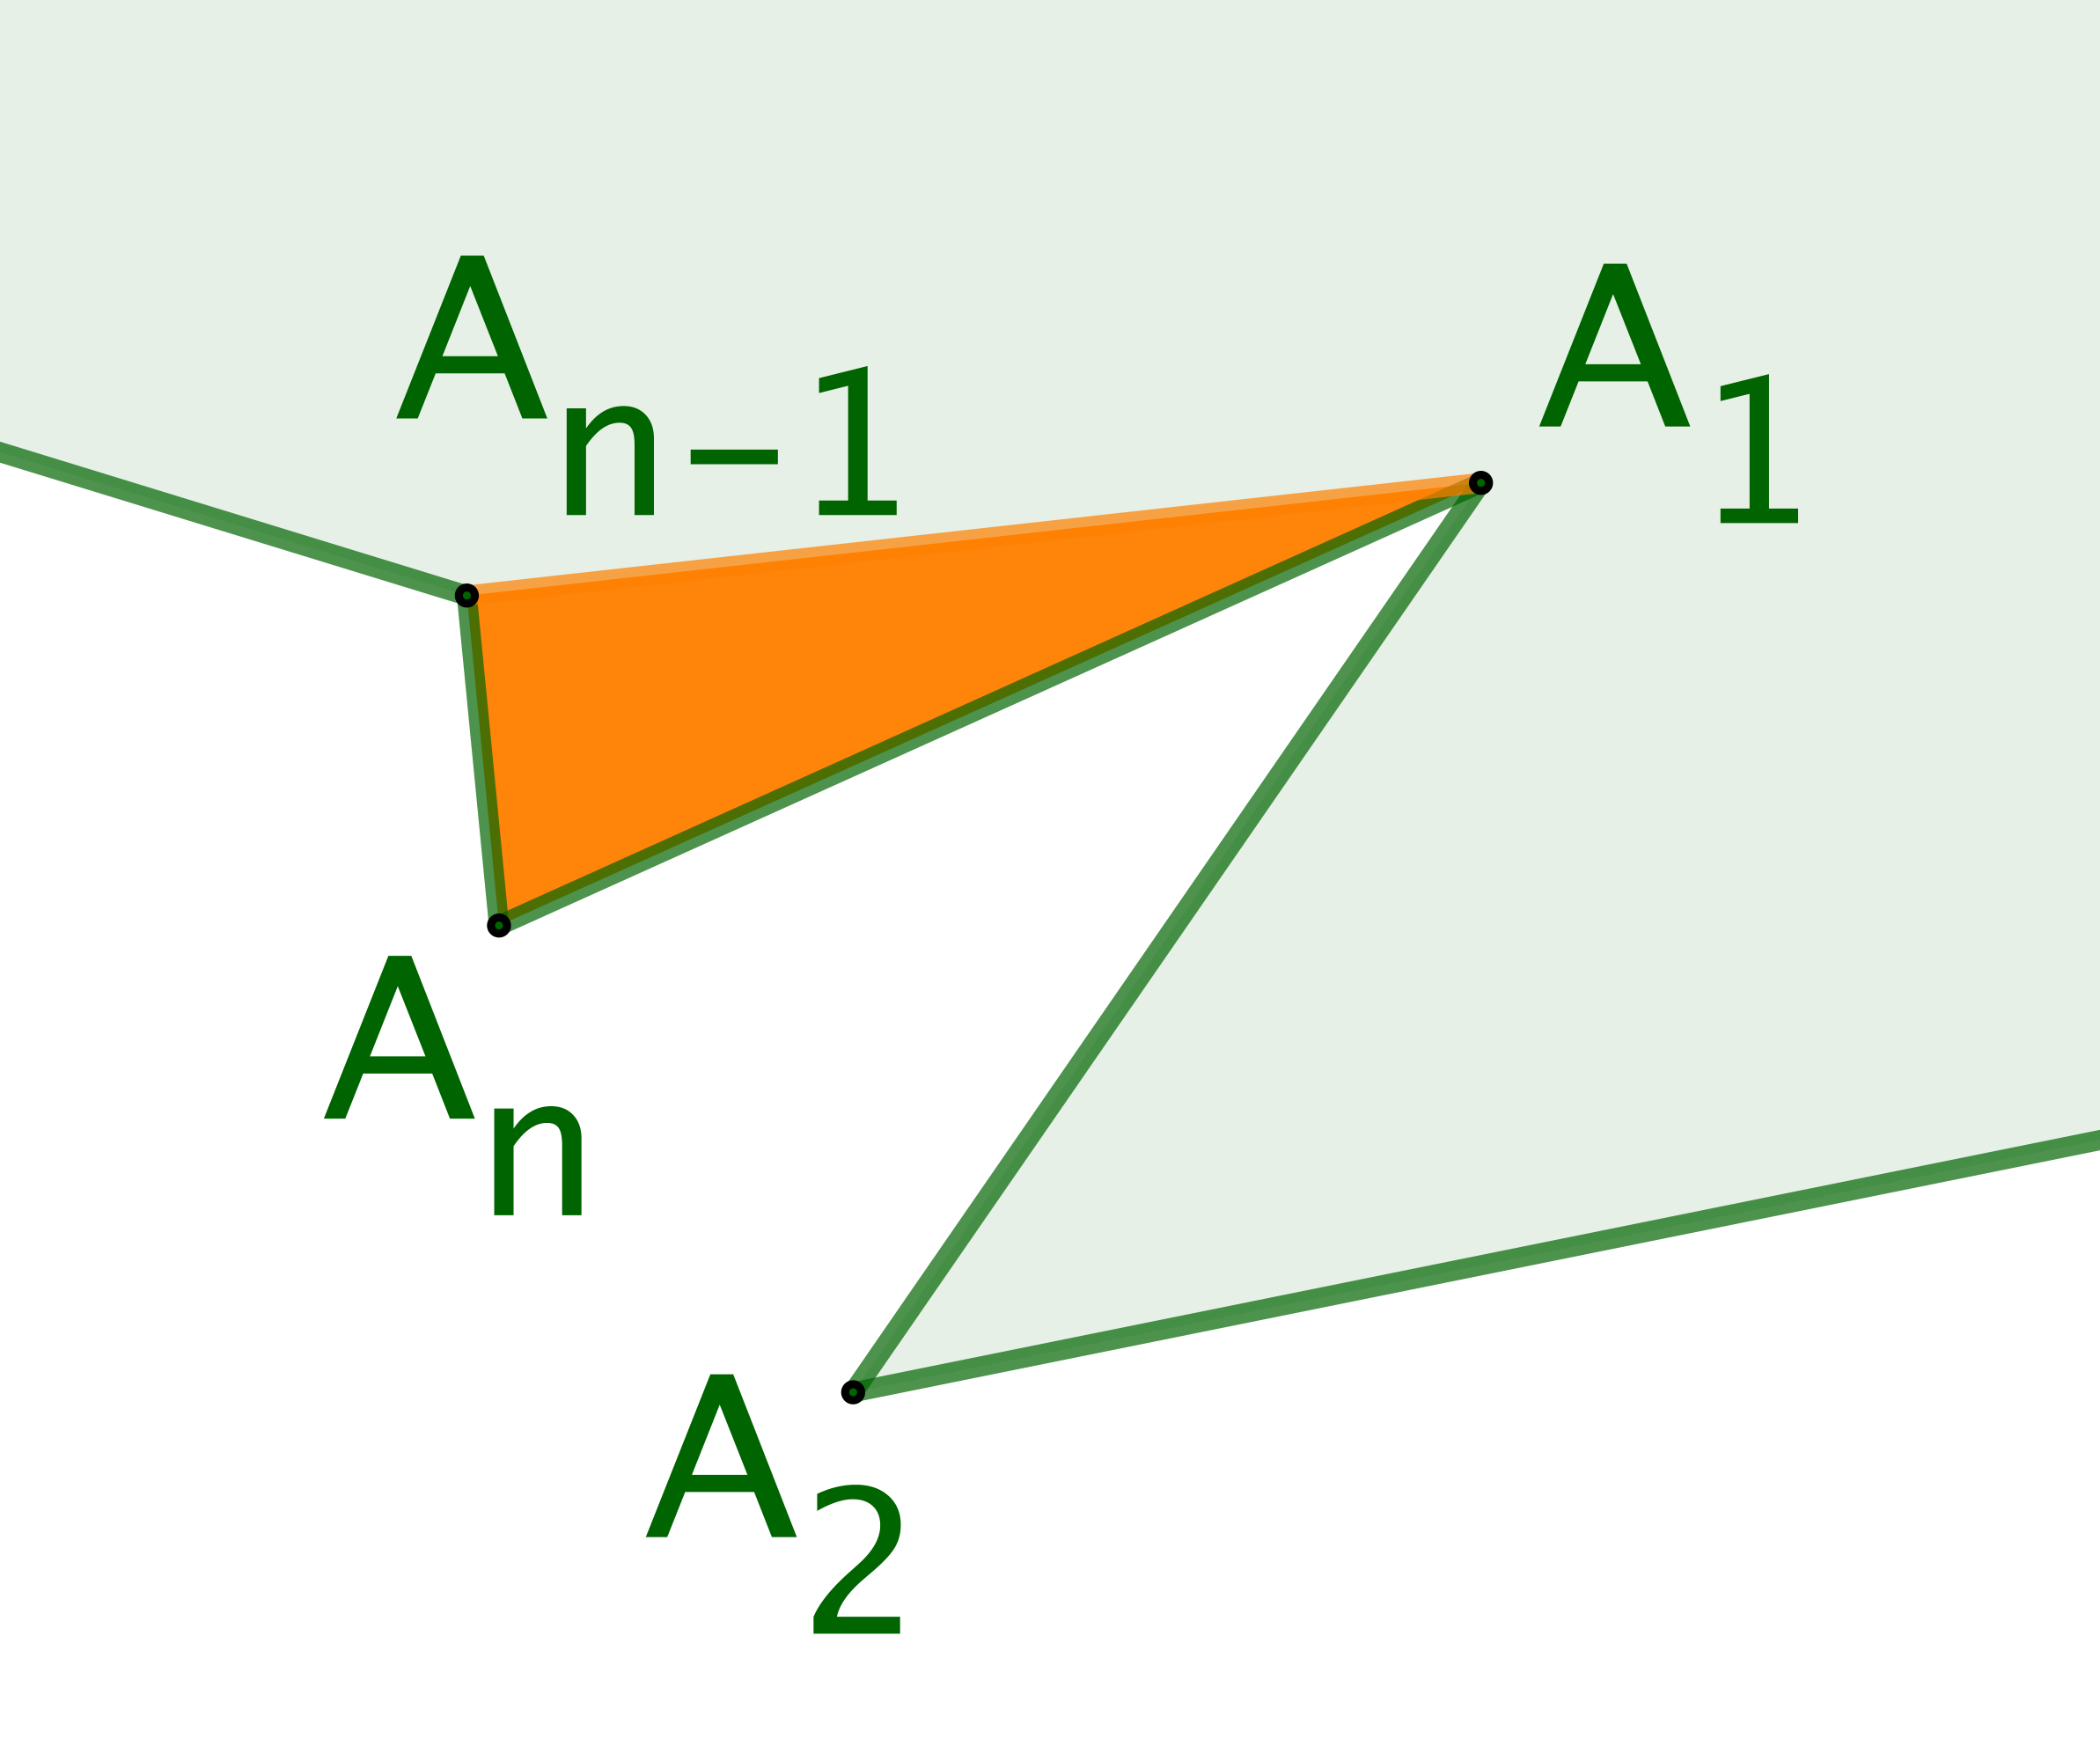
\includegraphics[scale=.4]{content/polygon/sufficient-cond/triangulation-proof.png}
    \end{center}
    
    
    Nous voilà prêt à raisonner par récurrence sur $n \in \NN_{\geq3}$.
    Le cas $n = 3$ ne posant aucune difficulté, nous allons juste considérer l'étape de récurrence en reprenant les notations précédentes.
    Soit ensuite
    $\setproba{P}^{\,\prime}$ le \kgone\ associé à la \kline\ $\setproba{L}^{\,\prime} = A_2 \cdots A_n$ où $k = n-1$ vérifie $k \in \NN_{\geq3}$.
    
    \begin{itemize}
    	\item $\area{\setproba{P}} = \area{A_1 A_{n-1} A_n}  +  \area{\setproba{P}^{\,\prime}}$, 
		car $A_1 A_{n-1} A_n$ est une oreille de $\setproba{P}$.


    	\item $\area{A_1 A_{n-1} A_n} = \garea{A_1 A_{n-1} A_n}$ et $\area{\setproba{P}^{\,\prime}} = \garea{\setproba{P}^{\,\prime}}$ 
		par récurrence.


    	\item Il n'est pas certain que $\garea{A_1 A_{n-1} A_n} + \garea{\setproba{P}^{\,\prime}} = \garea{\setproba{P}}$,
		du fait de l'utilisation de la valeur absolue pour définir une aire généralisée. Nous allons voir que c'est malgré tout le cas. 
		Quitte à changer de sens parcours de la frontière de $\setproba{P}$, et à renommer les sommets, 
		tout en utilisant $\Omega = A_n$ comme point de calcul,
		nous pouvons supposer que 
		$2 \garea{\setproba{P}^{\,\prime}}
		= \dsum_{j=1}^{n-2} \det \big( \vect{A_n A_j} , \vect{A_n A_{j + 1}} \big) 
		+ \det \big( \vect{A_n A_{n-1}} , \vect{A_n A_1} \big)$.
		Nous effectuons alors les calculs suivants.

		\leavevmode\kern-2em%
		\begin{stepcalc}[style=ar*]
			\pm 2 \garea{\setproba{P}}
		\explnext{Nous ne connaissons pas encore \\ le signe de la somme des déterminants.}
			\dsum_{j=1}^{n} \det \big( \vect{A_n A^{\,\prime}_j} ,  \vect{A_n A^{\,\prime}_{j + 1}} \big)
		\explnext{}
			\dsum_{j=1}^{n-2} \det \big( \vect{A_n A^{\,\prime}_j} , \vect{A_n A^{\,\prime}_{j + 1}} \big)
			+
			\det \big( \vect{A_n A^{\,\prime}_{n-1}} ,  \vect{A_n A^{\,\prime}_n} \big)
			+
			\det \big( \vect{A_n A^{\,\prime}_n} ,  \vect{A_n A^{\,\prime}_{n+1}} \big)
		\explnext*{$A_1 = A^{\,\prime}_{n+1}$ \\
		           $A_i = A^{\,\prime}_i$ \\ pour $i \leq n$}%
		          {}
			2 \garea{\setproba{P}^{\,\prime}}
			-
			\det \big( \vect{A_n A_{n-1}} , \vect{A_n A_1} \big)
		\explnext{}
			2 \garea{\setproba{P}^{\,\prime}}
			+
			\det \big( \vect{A_n A_1} , \vect{A_n A_{n-1}} \big)
		\end{stepcalc}
		
		\noindent
		Il faut donc justifier que nécessairement 
		$2 \garea{A_1 A_{n-1} A_n} = \det \big( \vect{A_n A_1} , \vect{A_n A_{n-1}} \big)$,
		car ceci donnera la positivité de la dernière somme qui sera donc égale à $2 \garea{\setproba{P}}$, puis nous aurons 
		$2 \garea{\setproba{P}} = 2 \garea{\setproba{P}^{\,\prime}} + 2 \garea{A_1 A_{n-1} A_n}$ 
		comme souhaité.
		
		
		
		XXXXX


    	\item Les points précédents donnent bien $\area{\setproba{P}} = \garea{\setproba{P}}$, ce qui achève notre démonstration par récurrence.
    \end{itemize}
\end{proof}


% ----------------------- %


\begin{fact} \label{no-cross-max}
    Si une \nline\ $\setproba{L}$ non dégénérée n'est pas un \ngone, donc est un polygone croisé, alors on peut construire un \ngone\ $\setproba{P}$ tel que 
	$\perim{\setproba{P}} = \perim{\setproba{L}}$ 
	et 
	$\garea{\setproba{P}} > \garea{\setproba{L}}$.
\end{fact}


\begin{proof}
	XXXX
\end{proof}



% ----------------------- %


\begin{fact} \label{suff-cond}
    Soit $n \in \NN_{\geq3}$ un naturel fixé.
    Considérons tous les \ngones\ de périmètre fixé. Parmi tous ces \ngones, il en existe au moins un d'aire maximale.
\end{fact}


\begin{proof}
	Ce qui suit nous donne plus généralement l'existence d'un \ngone, au moins, maximisant l'aire généralisée parmi toutes les \nlines\ de périmètre fixé $p$.
    %    
    \begin{itemize}
        \item On munit le plan d'un repère orthonormé direct $\pvaxes{O | i | j}$. 


        \item On considère $\setproba{Z}$ l'ensemble des \nlines\ $\setproba{L} = A_1 A_2 \cdots A_n$ vérifiant les propriétés suivantes.%
        \footnote{
        	Le mot \og \emph{Zeile} \fg\ est une traduction possible de \og \emph{ligne} \fg\ en allemand.
        }
        %
        \begin{enumerate}
        	\item $\perim{A_1 A_2 \cdots A_n} = p$

        	\item $A_1\coord{0 | 0}$
        \end{enumerate}


        \item Nous notons ensuite $\setproba{G} \subset \RR^{2n}$ l'ensemble des uplets $\big( x(A_1) ; y(A_1) ; \dots ; x(A_n) ; y(A_n) \big)$ correspondant aux coordonnées des sommets $A_i$ de \nlines\ appartenant à $\setproba{Z}$.
        
        
        \item $\setproba{G}$ est clairement fermé dans $\RR^{2n}$.
        De plus, il est borné, car les coordonnées des sommets des \nlines\ considérées le sont.        
        En résumé, $\setproba{G}$ est un compact de $\RR^{2n}$.


        \item Nous définissons la fonction $s: \setproba{G} \rightarrow \RRp$ qui à un uplet de $\setproba{G}$ associe l'aire généralisée de la \nline\ qu'il représente. 
        Cette fonction est continue comme valeur absolue d'une fonction polynomiale en les coordonnées.
       
        
        \item Finalement, par continuité et compacité, on sait que $s$ admet un maximum sur $\setproba{G}$.
        Or, un tel maximum ne peut être atteint en une \kline\ dégénérée, clairement, ni en un polygone croisé d'après le fait \ref{no-cross-max}, donc un tel maximum sera obtenu avec un \ngone. That's all folks!
    \end{itemize}    
\end{proof}


% ----------------------- %


\begin{fact}
    Soit $n \in \NN_{\geq3}$ un naturel fixé.
    Considérons tous les \ngones\  de périmètre fixé. Parmi tous ces \ngones, un seul est d'aire maximale, c'est le \ngone\ régulier.
\end{fact}


\begin{proof}
    Ceci découle directement des faits \ref{nece-cond} et \ref{suff-cond}.
    Ici s'achève notre joli voyage.
\end{proof}

\end{document}
